% ARTICLE ----
% This is just here so I know exactly what I'm looking at in Rstudio when messing with stuff.
\documentclass[11pt,]{article}
\usepackage[left=1in,top=1in,right=1in,bottom=1in]{geometry}
\newcommand*{\authorfont}{\fontfamily{phv}\selectfont}
\usepackage[]{mathpazo}


  \usepackage[T1]{fontenc}
  \usepackage[utf8]{inputenc}




\usepackage{abstract}
\renewcommand{\abstractname}{}    % clear the title
\renewcommand{\absnamepos}{empty} % originally center

\renewenvironment{abstract}
 {{%
    \setlength{\leftmargin}{0mm}
    \setlength{\rightmargin}{\leftmargin}%
  }%
  \relax}
 {\endlist}

\makeatletter
\def\@maketitle{%
  \newpage
%  \null
%  \vskip 2em%
%  \begin{center}%
  \let \footnote \thanks
    {\fontsize{18}{20}\selectfont\raggedright  \setlength{\parindent}{0pt} \@title \par}%
}
%\fi
\makeatother




\setcounter{secnumdepth}{0}

\usepackage{color}
\usepackage{fancyvrb}
\newcommand{\VerbBar}{|}
\newcommand{\VERB}{\Verb[commandchars=\\\{\}]}
\DefineVerbatimEnvironment{Highlighting}{Verbatim}{commandchars=\\\{\}}
% Add ',fontsize=\small' for more characters per line
\usepackage{framed}
\definecolor{shadecolor}{RGB}{248,248,248}
\newenvironment{Shaded}{\begin{snugshade}}{\end{snugshade}}
\newcommand{\AlertTok}[1]{\textcolor[rgb]{0.94,0.16,0.16}{#1}}
\newcommand{\AnnotationTok}[1]{\textcolor[rgb]{0.56,0.35,0.01}{\textbf{\textit{#1}}}}
\newcommand{\AttributeTok}[1]{\textcolor[rgb]{0.13,0.29,0.53}{#1}}
\newcommand{\BaseNTok}[1]{\textcolor[rgb]{0.00,0.00,0.81}{#1}}
\newcommand{\BuiltInTok}[1]{#1}
\newcommand{\CharTok}[1]{\textcolor[rgb]{0.31,0.60,0.02}{#1}}
\newcommand{\CommentTok}[1]{\textcolor[rgb]{0.56,0.35,0.01}{\textit{#1}}}
\newcommand{\CommentVarTok}[1]{\textcolor[rgb]{0.56,0.35,0.01}{\textbf{\textit{#1}}}}
\newcommand{\ConstantTok}[1]{\textcolor[rgb]{0.56,0.35,0.01}{#1}}
\newcommand{\ControlFlowTok}[1]{\textcolor[rgb]{0.13,0.29,0.53}{\textbf{#1}}}
\newcommand{\DataTypeTok}[1]{\textcolor[rgb]{0.13,0.29,0.53}{#1}}
\newcommand{\DecValTok}[1]{\textcolor[rgb]{0.00,0.00,0.81}{#1}}
\newcommand{\DocumentationTok}[1]{\textcolor[rgb]{0.56,0.35,0.01}{\textbf{\textit{#1}}}}
\newcommand{\ErrorTok}[1]{\textcolor[rgb]{0.64,0.00,0.00}{\textbf{#1}}}
\newcommand{\ExtensionTok}[1]{#1}
\newcommand{\FloatTok}[1]{\textcolor[rgb]{0.00,0.00,0.81}{#1}}
\newcommand{\FunctionTok}[1]{\textcolor[rgb]{0.13,0.29,0.53}{\textbf{#1}}}
\newcommand{\ImportTok}[1]{#1}
\newcommand{\InformationTok}[1]{\textcolor[rgb]{0.56,0.35,0.01}{\textbf{\textit{#1}}}}
\newcommand{\KeywordTok}[1]{\textcolor[rgb]{0.13,0.29,0.53}{\textbf{#1}}}
\newcommand{\NormalTok}[1]{#1}
\newcommand{\OperatorTok}[1]{\textcolor[rgb]{0.81,0.36,0.00}{\textbf{#1}}}
\newcommand{\OtherTok}[1]{\textcolor[rgb]{0.56,0.35,0.01}{#1}}
\newcommand{\PreprocessorTok}[1]{\textcolor[rgb]{0.56,0.35,0.01}{\textit{#1}}}
\newcommand{\RegionMarkerTok}[1]{#1}
\newcommand{\SpecialCharTok}[1]{\textcolor[rgb]{0.81,0.36,0.00}{\textbf{#1}}}
\newcommand{\SpecialStringTok}[1]{\textcolor[rgb]{0.31,0.60,0.02}{#1}}
\newcommand{\StringTok}[1]{\textcolor[rgb]{0.31,0.60,0.02}{#1}}
\newcommand{\VariableTok}[1]{\textcolor[rgb]{0.00,0.00,0.00}{#1}}
\newcommand{\VerbatimStringTok}[1]{\textcolor[rgb]{0.31,0.60,0.02}{#1}}
\newcommand{\WarningTok}[1]{\textcolor[rgb]{0.56,0.35,0.01}{\textbf{\textit{#1}}}}

\usepackage{graphicx,grffile}
\makeatletter
\def\maxwidth{\ifdim\Gin@nat@width>\linewidth\linewidth\else\Gin@nat@width\fi}
\def\maxheight{\ifdim\Gin@nat@height>\textheight\textheight\else\Gin@nat@height\fi}
\makeatother
% Scale images if necessary, so that they will not overflow the page
% margins by default, and it is still possible to overwrite the defaults
% using explicit options in \includegraphics[width, height, ...]{}
\setkeys{Gin}{width=\maxwidth,height=\maxheight,keepaspectratio}


\title{Career Promotion and Gender Disparities in Data Science: A Study
of European University Graduates on LinkedIn  }



\author{\Large Duc Tien Do, Yixin Mei, Anh Phuong
Dinh\vspace{0.05in} \newline\normalsize\emph{KU Leuven}  }


\date{}

\usepackage{titlesec}

\titleformat*{\section}{\normalsize\bfseries}
\titleformat*{\subsection}{\normalsize\itshape}
\titleformat*{\subsubsection}{\normalsize\itshape}
\titleformat*{\paragraph}{\normalsize\itshape}
\titleformat*{\subparagraph}{\normalsize\itshape}





\newtheorem{hypothesis}{Hypothesis}
\usepackage{setspace}


% set default figure placement to htbp
\makeatletter
\def\fps@figure{htbp}
\makeatother

\usepackage{booktabs}
\usepackage{longtable}
\usepackage{array}
\usepackage{multirow}
\usepackage{wrapfig}
\usepackage{float}
\usepackage{colortbl}
\usepackage{pdflscape}
\usepackage{tabu}
\usepackage{threeparttable}
\usepackage{threeparttablex}
\usepackage[normalem]{ulem}
\usepackage{makecell}
\usepackage{xcolor}

% move the hyperref stuff down here, after header-includes, to allow for - \usepackage{hyperref}

\makeatletter
\@ifpackageloaded{hyperref}{}{%
\ifxetex
  \PassOptionsToPackage{hyphens}{url}\usepackage[setpagesize=false, % page size defined by xetex
              unicode=false, % unicode breaks when used with xetex
              xetex]{hyperref}
\else
  \PassOptionsToPackage{hyphens}{url}\usepackage[draft,unicode=true]{hyperref}
\fi
}

\@ifpackageloaded{color}{
    \PassOptionsToPackage{usenames,dvipsnames}{color}
}{%
    \usepackage[usenames,dvipsnames]{color}
}
\makeatother
\hypersetup{breaklinks=true,
            bookmarks=true,
            pdfauthor={Duc Tien Do, Yixin Mei, Anh Phuong Dinh (KU
Leuven)},
             pdfkeywords = {LinkedIn, data scientist, job skill, career
progression, topic modelling, image processing, machine learning},
            pdftitle={Career Promotion and Gender Disparities in Data
Science: A Study of European University Graduates on LinkedIn},
            colorlinks=true,
            citecolor=blue,
            urlcolor=blue,
            linkcolor=magenta,
            pdfborder={0 0 0}}
\urlstyle{same}  % don't use monospace font for urls

% Add an option for endnotes. -----


% add tightlist ----------
\providecommand{\tightlist}{%
\setlength{\itemsep}{0pt}\setlength{\parskip}{0pt}}

% add some other packages ----------

% \usepackage{multicol}
% This should regulate where figures float
% See: https://tex.stackexchange.com/questions/2275/keeping-tables-figures-close-to-where-they-are-mentioned
\usepackage[section]{placeins}

% CSL environment change -----


% Last minute stuff -----
\usepackage{amssymb,amsmath} % HT @ashenkin


\begin{document}

% \pagenumbering{arabic}% resets `page` counter to 1
%
% \maketitle

{% \usefont{T1}{pnc}{m}{n}
\setlength{\parindent}{0pt}
\thispagestyle{plain}
{\fontsize{18}{20}\selectfont\raggedright
\maketitle  % title \par

}

{
   \vskip 13.5pt\relax \normalsize\fontsize{11}{12}
\textbf{\authorfont Duc Tien Do, Yixin Mei, Anh Phuong
Dinh} \hskip 15pt \emph{\small KU Leuven}   

}

}








\begin{abstract}

    \hbox{\vrule height .2pt width 39.14pc}

    \vskip 8.5pt % \small

\noindent In the fiercely competitive landscape of information
technology and data science, the increasing requirements for
professionals have led to questions about the factors that distinguish
successful career progression. To explore these questions, we conducted
an analysis examining the LinkedIn profiles of over 10,000 alumni from
major European universities specialising in data science, statistics,
software engineering, and artificial intelligence. Our notebook employed
various machine learning and statistical techniques, such as image
recognition, topic modelling, and ensemble models, to investigate how
gender, networking, education, language, and technical skills have an
association with career promotions. Additionally, we explored potential
gender disparities between male and female professionals in relation to
these factors. The key findings revealed significant disparities in
career progression based on gender. Moreover, the level of education,
networking abilities, and certain language skills and professtional
skills were identified as factors with significant assocation with
different career trajectories.


\vskip 8.5pt \noindent \emph{Keywords}: LinkedIn, data scientist, job
skill, career progression, topic modelling, image processing, machine
learning \par

    \hbox{\vrule height .2pt width 39.14pc}



\end{abstract}


\vskip -8.5pt


 % removetitleabstract

\noindent 

\hypertarget{introduction}{%
\section{Introduction}\label{introduction}}

In today's rapidly evolving professional landscape, comprehending the
association between various factors and career progression is crucial
for both individuals and institutions, especially in dynamic fields like
data science and artificial intelligence. In these domains,
professionals must continuously update their skill sets to stay relevant
and adapt to the ever-changing market demands. Therefore, it becomes
even more crucial to comprehend the elements that contribute to
successful career trajectories.

This project seeks to explore the association of gender, networking,
internships, and technical skills with the career progression of
graduates from reputable European universities specializing in
statistics, data science, and artificial intelligence. To achieve this,
we will leverage the valuable insights provided by LinkedIn data, which
offers comprehensive professional profiles and experiences.
Understanding the assocation of these factors will be essential for
individuals seeking successful careers in these fields, as well as for
institutions aiming to support the professional growth of their
graduates.

\hypertarget{literature-review-and-hypotheses-development}{%
\section{Literature review and Hypotheses
development}\label{literature-review-and-hypotheses-development}}

\hypertarget{gender-and-managerial-roles}{%
\subsection{Gender and Managerial
Roles:}\label{gender-and-managerial-roles}}

Although significant progress has been made towards gender equality in
various professional domains, research consistently documents
gender-related disparities, particularly in fields traditionally
dominated by men, such as science, technology, and math. Evidence shows
that women applicants in STEM are less likely to be hired and receive
lower starting salaries than men with identical records (Moss-Racusin et
al., 2012). In addition, while people drop out of a pathway towards
STEM-related careers at various time points, females are generally more
likely to drop out than males (Watt \& Eccles, 2008).

Furthermore, female representation is particularly limited in
math-intensive science fields like geosciences, engineering, economics,
math/computer science, and physical science (Kahn \& Ginther, 2017) --
limited research specifically focuses on the career progression of
female graduates in data science, statistics, and artificial
intelligence. As a result, our study aims to address this gap and
provide insights into the unique challenges and opportunities faced by
women in these fields.

We expect that there may be gender disparities in managerial roles
within the data science and AI fields. Specifically, women may be less
likely to hold senior management positions compared to their male
counterparts. This could be due to various factors, including gender
biases, societal norms, and potential differences in self-promotion and
negotiation styles.

\hypertarget{networking-and-career-advancement}{%
\subsection{Networking and Career
Advancement:}\label{networking-and-career-advancement}}

The number of connections and followers on LinkedIn is an indicator of
networking skills and is relevant for various jobs, including
recruiting, marketing, sales, or public relations (Zide et al., 2014).
Having more connections makes it easier for individuals to be found by
recruiters or hiring managers conducting keyword-based searches
(Schneiderman, 2016). Recruiters can also analyze the connections of
their existing employees to identify potential candidates for job
vacancies (Caers \& Castelyns, 2011). Therefore, building and nurturing
professional connections can lead to job opportunities, mentorship, and
other benefits. We will examine the association between networking on
career promotions based on the ``connection'' feature on LinkedIn.

\hypertarget{internship-experience-and-career-advancement}{%
\subsection{Internship Experience and Career
Advancement:}\label{internship-experience-and-career-advancement}}

The relevance and quality of internships greatly impact the career paths
of graduates as they bridge the gap between academia and industry.
Internship experiences provide benefits such as a better matching and
selection process for interns and potential employers and the
development of professional skills, knowledge, and socialization (Rigsby
et al., 2013).

We expect that graduates who have completed internships or student work
placements will have a positive correlation with the likelihood of
getting promoted. Practical experience gained during internships may
increase employability and lead to more favorable career trajectories
compared to those without such experiences.

\hypertarget{technical-skills-and-career-advancement}{%
\subsection{Technical Skills and Career
Advancement:}\label{technical-skills-and-career-advancement}}

In the fields of statistics, data science, and artificial intelligence,
technical skills are essential. According to Coursera platform,
proficiency in programming, statistics and probability, machine
learning, cloud computing, and related areas directly impacts career
prospects. Identifying patterns in the skills held by graduates will
provide insights into the essential skills for data-driven work.

We hypothesize a positive correlation between the level of technical
proficiency and career promotion. Graduates who possess advanced
technical skills and expertise in relevant programming languages, tools,
and methodologies are likely to experience faster career progression
compared to those with more limited technical abilities.

\hypertarget{research-questions}{%
\section{Research questions}\label{research-questions}}

With our research interests and the aforementioned hypotheses as a
foundation, our study seeks to address the following research questions:

\begin{enumerate}
\def\labelenumi{\arabic{enumi}.}
\item
  Which factors demonstrate significant associations with the likelihood
  of receiving promotions within the data science, IT, software, and
  artificial intelligence sectors?
\item
  What attributes set apart the profiles of male and female
  professionals in these fields?
\end{enumerate}

\hypertarget{sub-questions}{%
\subsection{Sub-questions:}\label{sub-questions}}

\begin{enumerate}
\def\labelenumi{\arabic{enumi}.}
\item
  What are the prevailing industries with which these professionals
  associate themselves on LinkedIn?
\item
  What are the common job titles among these professionals?
\item
  What (sub-)topics can be discerned from the skill sets demonstrated by
  these professionals on their profiles?
\end{enumerate}

\hypertarget{methodology}{%
\section{Methodology}\label{methodology}}

For data acquisition, we utilized Selenium, Beautiful Soup, and the
open-source LinkedIn API to perform web scraping and collect profile
data of alumni from ten reputable European universities. The
universities included are KU Leuven, University of Antwerp, Ghent
University, Leiden University, University of Groningen, Utrecht
University, Technical University of Munich, RWTH Aachen University,
University of Amsterdam, Delft University of Technology, and Ludwig
Maximilian University. To ensure relevance to our study, we used
specific keywords such as ``Data scientist,'' ``Data analyst,'' ``Data
engineer,'' ``Machine learning engineer,'' ``Statistician,'' ``Python
developer,'' ``Research analyst,'' ``Artificial intelligence engineer,''
and ``NLP engineer'' in refining our search.

To investigate potential gender disparities or biases within the fields
of interest, our study incorporated gender classification based on
profile photos. As explicit gender information is often absent on
LinkedIn profiles, we relied on the Deepface library for image
classification. This is a robust Python library specifically designed
for facial recognition and facial attribute analysis, offering
pre-trained deep learning models trained on large-scale facial datasets,
including VGG-Face, Google Facenet, OpenFace, and others. Despite our
limited and highly unbalanced dataset, Deepface's powerful models
enabled us to tackle the challenging task of image classification
efficiently, eliminating the need for manual data labelling. The quality
and characteristics of LinkedIn profile photos further support the
suitability of Deepface for this task. LinkedIn photos are typically of
high-quality, well-lit, and centered on the individual's face. These
favourable attributes make them an ideal input for facial analysis,
leading us to anticipate the level of performance and accuracy from
Deepface in this task to be beyond satisfactory. However, to ensure
optimal input for the ensemble model, we also performed a manual visual
check on the predictions from Deepface to correct any misclassified
observations.

The essential data manipulation and transformation steps will be carried
out in the R environment, involving cleaning, organizing, and
structuring the data to ensure its suitability for analysis. Further
details regarding ethical practices will be provided in the subsequent
section.

In the tech industry, the importance of skills, especially hard skills,
on a LinkedIn profile cannot be overstated. Topic modeling will be
utilized as an ideal approach for feature engineering to handle the
extensive diversity of skills displayed on LinkedIn profiles. This
statistical technique uncovers underlying topics or themes within the
text data (skills listed on profiles) automatically. Through topic
modeling, distinct clusters of skills that individuals possess can be
identified without predefined categories. The advantages lie in its
ability to extract latent patterns and associations within the skills
data, capturing diverse skill sets prevalent in the tech industry,
including technical, programming, and domain-specific skills.

To address the research questions, we will employ XGBoost and Logistic
Regression. Moreover, to enhance interpretability, XGBoost will be
combined with the SHAP (SHapley Additive exPlanations) technique, which
will provide insights into the contribution of individual features to
the models' predictions.

\hypertarget{ethics}{%
\subsection{Ethics}\label{ethics}}

This research project involves analyzing publicly available LinkedIn
data, specifically information that users have shared on their public
profiles.

Given that the data used in this study is publicly accessible and does
not necessitate direct interaction with LinkedIn users, we have not
actively sought explicit consent from them for its use in our research.
However, we emphasize our respect for the privacy and preferences of all
LinkedIn users and want to assure that no data that could lead to
individual identification has been shared or employed for purposes
beyond the scope of this academic study. We recognize that merely
pseudonymizing and eliminating personally identifiable particulars such
as names, contact details, and LinkedIn user IDs may not suffice to
ensure user privacy and users can still potentially be traced back
through information such as school names, job titles, and company
affiliations. Therefore, we have taken a rigorous process of data
aggregation, retaining only essential information in the final dataset
to prevent any tracking of specific individuals.

We are dedicated to conducting this research with full respect for
individuals' privacy and rights. The outcomes of this study will be used
solely for academic purposes.

\hypertarget{tools}{%
\section{Tools}\label{tools}}

For the technical aspects of the study, both Python and R programming
languages were employed. Python was chosen specifically for data
collection, image processing and translation tasks due to the
availability of necessary APIs and libraries that are not readily
accessible in R. As this notebook is written in Rmarkdown, the lines of
Python code provided are solely intended for demonstration purposes and
not recommended to be run.

\hypertarget{python-tools}{%
\subsection{Python tools}\label{python-tools}}

The following commands are executed in the command prompt/ terminal in
order to verify the installation of Python and pip on the system.

\begin{Shaded}
\begin{Highlighting}[]
\NormalTok{python }\OperatorTok{{-}{-}}\NormalTok{version}
\NormalTok{pip }\OperatorTok{{-}{-}}\NormalTok{version}
\end{Highlighting}
\end{Shaded}

After confirming the presence of Python and pip, the installation of the
necessary libraries can be proceeded by running the following commands.

\begin{Shaded}
\begin{Highlighting}[]
\NormalTok{pip install pandas}
\NormalTok{pip install selenium}
\NormalTok{pip install linkedin\_api}
\NormalTok{pip install deepface}
\NormalTok{pip install opencv}\OperatorTok{{-}}\NormalTok{python}
\NormalTok{pip install matplotlib}
\NormalTok{pip install urllib3}
\NormalTok{pip install langdetect googletrans}\OperatorTok{==}\FloatTok{4.0.0}\OperatorTok{{-}}\NormalTok{rc1}
\end{Highlighting}
\end{Shaded}

Once the installations are complete, importing the required libraries
into the script or Jupyter Notebook is possible.

\begin{Shaded}
\begin{Highlighting}[]
\ImportTok{import}\NormalTok{ os, random, sys, time }

\CommentTok{\# Data scraping}
\ImportTok{from}\NormalTok{ selenium }\ImportTok{import}\NormalTok{ webdriver}
\ImportTok{from}\NormalTok{ linkedin\_api }\ImportTok{import}\NormalTok{ Linkedin}
\ImportTok{from}\NormalTok{ bs4 }\ImportTok{import}\NormalTok{ BeautifulSoup}
\ImportTok{import}\NormalTok{ requests}
\ImportTok{from}\NormalTok{ urllib.request }\ImportTok{import}\NormalTok{ urlopen}

\CommentTok{\# Data manipulation and visualization}
\ImportTok{import}\NormalTok{ pandas }\ImportTok{as}\NormalTok{ pd}
\ImportTok{import}\NormalTok{ json}
\ImportTok{import}\NormalTok{ numpy }\ImportTok{as}\NormalTok{ np}
\ImportTok{import}\NormalTok{ json}
\ImportTok{import}\NormalTok{ matplotlib.pyplot }\ImportTok{as}\NormalTok{ plt}

\CommentTok{\# Image recognition}
\ImportTok{from}\NormalTok{ deepface }\ImportTok{import}\NormalTok{ DeepFace}
\ImportTok{import}\NormalTok{ cv2}

\CommentTok{\# Translation language}
\ImportTok{from}\NormalTok{ googletrans }\ImportTok{import}\NormalTok{ Translator}
\end{Highlighting}
\end{Shaded}

\hypertarget{r-tools}{%
\subsection{R tools}\label{r-tools}}

The following command are executed to install and import the necessary R
package for our analyzing and modeling.

\begin{Shaded}
\begin{Highlighting}[]
\CommentTok{\# install package}

\NormalTok{package\_install }\OtherTok{=} \FunctionTok{c}\NormalTok{(}\StringTok{"tidyverse"}\NormalTok{,}
                    \StringTok{"jsonlite"}\NormalTok{,}
                    \StringTok{"tokenizers"}\NormalTok{,}
                    \StringTok{"tidytext"}\NormalTok{,}
                    \StringTok{"quanteda"}\NormalTok{, }
                    \StringTok{"lubridate"}\NormalTok{,}
                    \StringTok{"textplot"}\NormalTok{,}
                    \StringTok{"scales"}\NormalTok{,}
                    \StringTok{"tm"}\NormalTok{,}
                    \StringTok{"topicmodels"}\NormalTok{,}
                    \StringTok{"spacyr"}\NormalTok{,}
                    \StringTok{"textstem"}\NormalTok{,}
                    \StringTok{"kableExtra"}\NormalTok{,}
                    \StringTok{"LDAvis"}\NormalTok{,}
                    \StringTok{"quanteda.textplots"}\NormalTok{,}
                    \StringTok{"stats"}\NormalTok{,}
                    \StringTok{"ldatuning"}\NormalTok{,}
                    \StringTok{"caret"}\NormalTok{,}
                    \StringTok{"xgboost"}\NormalTok{,}
                    \StringTok{"ROSE"}\NormalTok{,}
                    \StringTok{"fastDummies"}\NormalTok{)}

\ControlFlowTok{for}\NormalTok{ (package\_name }\ControlFlowTok{in}\NormalTok{ package\_install)\{}
\ControlFlowTok{if}\NormalTok{(}\SpecialCharTok{!}\FunctionTok{requireNamespace}\NormalTok{(package\_name, }\AttributeTok{quietly =} \ConstantTok{TRUE}\NormalTok{))\{}
  \FunctionTok{install.packages}\NormalTok{(package\_name)}
\NormalTok{\}}

\NormalTok{\}}
\end{Highlighting}
\end{Shaded}

\begin{Shaded}
\begin{Highlighting}[]
\CommentTok{\# import package}
\DocumentationTok{\#\# Data manipulation and visualization}
\FunctionTok{library}\NormalTok{(tidyverse)}
\FunctionTok{library}\NormalTok{(jsonlite)}
\FunctionTok{library}\NormalTok{(fastDummies)}
\FunctionTok{library}\NormalTok{(lubridate)}
\FunctionTok{library}\NormalTok{(stats)}
\FunctionTok{library}\NormalTok{(dplyr)}
\FunctionTok{library}\NormalTok{(ggplot2)}
\FunctionTok{library}\NormalTok{(scales)}
\FunctionTok{library}\NormalTok{(reshape2)}
\FunctionTok{library}\NormalTok{(stringr)}

\DocumentationTok{\#\# Topic modelling/Text mining }
\FunctionTok{library}\NormalTok{(tidytext)}
\FunctionTok{library}\NormalTok{(quanteda)}
\FunctionTok{library}\NormalTok{(textplot)}
\FunctionTok{library}\NormalTok{(topicmodels)}
\FunctionTok{library}\NormalTok{(tokenizers)}
\FunctionTok{library}\NormalTok{(textstem)}
\FunctionTok{library}\NormalTok{(LDAvis)}
\FunctionTok{library}\NormalTok{(quanteda.textplots)}
\FunctionTok{library}\NormalTok{(ldatuning)}
\FunctionTok{library}\NormalTok{(spacyr)}
\FunctionTok{library}\NormalTok{(tm)}
\FunctionTok{library}\NormalTok{(wordcloud)}

\DocumentationTok{\#\# Modeling}
\FunctionTok{library}\NormalTok{(caret)}
\FunctionTok{library}\NormalTok{(xgboost)}
\FunctionTok{library}\NormalTok{(ROSE)}
\FunctionTok{library}\NormalTok{(MASS)}

\DocumentationTok{\#\# Markdown }
\FunctionTok{library}\NormalTok{(kableExtra)}
\FunctionTok{library}\NormalTok{(knitr)   }
\end{Highlighting}
\end{Shaded}

\hypertarget{data-acquisition}{%
\section{Data Acquisition}\label{data-acquisition}}

This section focuses on the data collection process from LinkedIn
profiles, which involves two steps. Firstly, we manually collect the
profile URLs, which contain the public IDs, from LinkedIn. Subsequently,
we extract the necessary information from each profile by utilizing its
corresponding public ID.

\hypertarget{collecting-profile-urls-public-ids}{%
\subsection{Collecting profile URLs/ public
IDs}\label{collecting-profile-urls-public-ids}}

To collect data from LinkedIn, it is necessary to set up a LinkedIn
account which provides access to the platform. The data collection
process begins by setting up the WebDriver using the Selenium library in
Python, specifically, the Chrome WebDriver, which facilitates automated
web browsing. The browser is then directed to the LinkedIn login page
where the required login credentials should be entered, granting access
to the platform.

\begin{Shaded}
\begin{Highlighting}[]
\NormalTok{browser }\OperatorTok{=}\NormalTok{ webdriver.Chrome(}\StringTok{\textquotesingle{}/driver/chromedriver\textquotesingle{}}\NormalTok{)}
\NormalTok{browser.get(}\StringTok{"https://www.linkedin.com/login/"}\NormalTok{)}
\end{Highlighting}
\end{Shaded}

After gaining access to the LinkedIn platform, the browser proceeded to
navigate to the desired LinkedIn page by providing the relevant URL. For
the purpose of our report, we aimed to examine alumni from European
institutions offering programs in data science, statistics, and
artificial intelligence. The institutions included in our search were KU
Leuven, University of Antwerp, Ghent University, Leiden University,
University of Groningen, Utrecht University, Technical University of
Munich, RWTH Aachen University, University of Amsterdam, Delft
University of Technology, and Ludwig Maximilian University. To refine
our search and target alumni in the relevant fields, we used specific
keywords such as \texttt{Data\ scientist}, \texttt{Data\ analyst},
\texttt{Data\ engineer}, \texttt{Machine\ learning\ engineer},
\texttt{Statistician}, \texttt{Python\ developer},
\texttt{Research\ analyst}, \texttt{Artificial\ intelligence\ engineer},
and \texttt{NLP\ engineer}. In this case, the provided URL led to the KU
Leuven school page with customized filters applied for the specific
keywords to narrow down the search.

\begin{Shaded}
\begin{Highlighting}[]
\NormalTok{browser.get(paste(}\StringTok{"https://www.linkedin.com/school/ku\_leuven/people/?keywords="}\NormalTok{,}
                  \StringTok{"Data}\SpecialCharTok{\%20s}\StringTok{cientist\%20OR}\SpecialCharTok{\%20d}\StringTok{ata\%20analyst\%20OR}\SpecialCharTok{\%20d}\StringTok{ata}\SpecialCharTok{\%20e}\StringTok{ngineer\%"}\NormalTok{,}
                  \StringTok{"20OR\%20machine}\SpecialCharTok{\%20le}\StringTok{arning}\SpecialCharTok{\%20e}\StringTok{ngineer\%20OR}\SpecialCharTok{\%20s}\StringTok{tatistician"}\NormalTok{, }
\NormalTok{                  sep }\OperatorTok{=} \StringTok{""}\NormalTok{))}
\end{Highlighting}
\end{Shaded}

To ensure that the entire LinkedIn page is loaded and that all the
desired content is available for data collection, the browser executed
JavaScript code to scroll through the entire page, repeating this
process a predetermined number of times.

\begin{Shaded}
\begin{Highlighting}[]
\NormalTok{rep }\OperatorTok{=} \DecValTok{100}
\NormalTok{last\_height }\OperatorTok{=}\NormalTok{ browser.execute\_script(}\StringTok{"return document.body.scrollHeight"}\NormalTok{)}

\ControlFlowTok{for}\NormalTok{ i }\KeywordTok{in} \BuiltInTok{range}\NormalTok{(rep):}
\NormalTok{    browser.execute\_script(}\StringTok{\textquotesingle{}window.scrollTo(0, document.body.scrollHeight);\textquotesingle{}}\NormalTok{)}
\NormalTok{    time.sleep(}\DecValTok{5}\NormalTok{)}
\NormalTok{    new\_height }\OperatorTok{=}\NormalTok{ browser.execute\_script(}\StringTok{"return document.body.scrollHeight"}\NormalTok{)}
    \ControlFlowTok{if}\NormalTok{ new\_height }\OperatorTok{==}\NormalTok{ last\_height:}
        \ControlFlowTok{break}
\NormalTok{    new\_height }\OperatorTok{=}\NormalTok{ last\_height}
\end{Highlighting}
\end{Shaded}

Lastly, the page source was extracted, and the relevant section
containing the profile URLs was identified based on specific HTML tags
and attributes. The profile IDs were then extracted from the URLs and
stored in a list. Finally, the collected IDs were organized into a
DataFrame and saved as a CSV file for further step.

\begin{Shaded}
\begin{Highlighting}[]
\NormalTok{src }\OperatorTok{=}\NormalTok{ browser.page\_source}
\NormalTok{soup }\OperatorTok{=}\NormalTok{ BeautifulSoup(src, }\StringTok{\textquotesingle{}lxml\textquotesingle{}}\NormalTok{)}
\NormalTok{pav }\OperatorTok{=}\NormalTok{ soup.find(}\StringTok{\textquotesingle{}div\textquotesingle{}}\NormalTok{, \{}\StringTok{\textquotesingle{}class\textquotesingle{}}\NormalTok{ : }\StringTok{\textquotesingle{}scaffold{-}finite{-}scroll\_\_content\textquotesingle{}}\NormalTok{\})}
\NormalTok{all\_links }\OperatorTok{=}\NormalTok{ pav.find\_all(}\StringTok{\textquotesingle{}a\textquotesingle{}}\NormalTok{, \{}\StringTok{\textquotesingle{}class\textquotesingle{}}\NormalTok{ : }\StringTok{"app{-}aware{-}link"}\NormalTok{\})}
\NormalTok{profile\_url }\OperatorTok{=}\NormalTok{ [link.get(}\StringTok{"href"}\NormalTok{) }\ControlFlowTok{for}\NormalTok{ link }\KeywordTok{in}\NormalTok{ all\_links]}
\NormalTok{profile\_id }\OperatorTok{=}\NormalTok{ [url.split(}\StringTok{"?"}\NormalTok{)[}\DecValTok{0}\NormalTok{] }\ControlFlowTok{for}\NormalTok{ url }\KeywordTok{in}\NormalTok{ profile\_url]}
\NormalTok{profile\_id }\OperatorTok{=} \BuiltInTok{list}\NormalTok{(}\BuiltInTok{set}\NormalTok{(profile\_id)) }\CommentTok{\# remove duplicates}
\NormalTok{all\_id }\OperatorTok{=}\NormalTok{ pd.DataFrame(profile\_id, columns}\OperatorTok{=}\NormalTok{[}\StringTok{\textquotesingle{}ID\textquotesingle{}}\NormalTok{])}
\NormalTok{all\_id.to\_csv(}\StringTok{\textquotesingle{}all\_id.csv\textquotesingle{}}\NormalTok{)}
\end{Highlighting}
\end{Shaded}

\hypertarget{extracting-information-from-profile-ids}{%
\subsection{Extracting information from profile
IDs}\label{extracting-information-from-profile-ids}}

Thanks to the open-source \texttt{linkedin\_api}, the process becomes
much more streamlined and straightforward compared to the previous step.
First, authentication is performed by creating an instance of the
LinkedIn class and passing the LinkedIn account credentials.

\begin{Shaded}
\begin{Highlighting}[]
\ImportTok{from}\NormalTok{ linkedin\_api }\ImportTok{import}\NormalTok{ Linkedin}

\CommentTok{\# Authenticate using any Linkedin account credentials}
\NormalTok{api }\OperatorTok{=}\NormalTok{ Linkedin(email, password) }\CommentTok{\# Enter the email and password of your account}
\end{Highlighting}
\end{Shaded}

Next, a dictionary is initialized to store the profile information of
LinkedIn users. Within a loop iterating over the user IDs,
\texttt{linkedin\_api} is utilized to retrieve the respective profile
information and network information specific to each user. The obtained
profile information, along with the corresponding network information,
is then stored in the dictionary using the user ID as the key. Lastly,
the dictionary is dumped into a JSON file, which will serve as the final
dataset for further analysis.

\begin{Shaded}
\begin{Highlighting}[]
\NormalTok{profiles }\OperatorTok{=}\NormalTok{ \{\}}

\ControlFlowTok{for}\NormalTok{ user }\KeywordTok{in}\NormalTok{ all\_id:}
\NormalTok{    profile\_info }\OperatorTok{=}\NormalTok{ api.get\_profile(user)}
\NormalTok{    profile\_info[}\StringTok{\textquotesingle{}network\textquotesingle{}}\NormalTok{] }\OperatorTok{=}\NormalTok{ api.get\_profile\_network\_info(user)}
\NormalTok{    profiles[user] }\OperatorTok{=}\NormalTok{ profile\_info}

\ControlFlowTok{with} \BuiltInTok{open}\NormalTok{(}\StringTok{\textquotesingle{}all\_profiles.json\textquotesingle{}}\NormalTok{, }\StringTok{\textquotesingle{}w\textquotesingle{}}\NormalTok{) }\ImportTok{as}\NormalTok{ f:}
\NormalTok{    json.dump(all\_profiles, f)}
\end{Highlighting}
\end{Shaded}

An instance of user information that we collect from Linkedin using
\texttt{linkedin\_api} would be presented in the following link
\url{https://github.com/tiendd712/Socialscience_bigdata_KUL/blob/master/Assignment\%203/linkedin_scraper/profiles_demo.json}

\hypertarget{data-preprocessing}{%
\section{Data Preprocessing}\label{data-preprocessing}}

\hypertarget{data-extraction}{%
\subsection{Data Extraction}\label{data-extraction}}

The data obtained from LinkedIn was in dictionary format and contained
various information. To address this, we extracted only the meaningful
details from the dictionary and converted them into data frames. This
conversion to data frames facilitated easier data handling and analysis.
We organized the data into distinct frames, each representing specific
information, such as the number of followers, number of connections,
experience, education, skills, language, profile picture, and
self-summary.

Regarding number of connections data, we observed that the number of
connections on Linkedin is capped at 500, which means those with 500+
connections are still recorded as having 500 connections in our data
set. Acknowledging this limitation, we chose to categorize the
connection variable into a binary format, where \texttt{1} indicates the
user possesses 500 or more connections, and \texttt{0} otherwise. To
maintain brevity and conciseness in the report, we will provide the code
for data preprocessing through the following link:
\url{https://github.com/tiendd712/Socialscience_bigdata_KUL/blob/master/Assignment\%203/data_processing/data_processing_final.R}

\hypertarget{text-translation}{%
\subsection{Text Translation}\label{text-translation}}

We utilized the \texttt{googletrans} library in Python, which
incorporates the Google Translate API, to handle profiles written in
languages other than English, such as German, Dutch, or French. The
library's significant advantage is its ability to automatically detect
the language and provide translations into English. However, the
translation process can be time-consuming. Given our time constraints,
we used the translation exclusively for skill data, as it is necessary
to provide a consistent format for feature engineering. The following
Python code illustrates the process.

\begin{Shaded}
\begin{Highlighting}[]
\NormalTok{translator }\OperatorTok{=}\NormalTok{ Translator()}

\NormalTok{skill\_data[}\StringTok{"skill\_trans"}\NormalTok{] }\OperatorTok{=} \StringTok{"1"}


\ControlFlowTok{for}\NormalTok{ i }\KeywordTok{in} \BuiltInTok{range}\NormalTok{(}\DecValTok{0}\NormalTok{,}\BuiltInTok{len}\NormalTok{(skill\_data[}\StringTok{"skills"}\NormalTok{])):}
  \ControlFlowTok{if}\NormalTok{ skill\_data.iloc[i, }\DecValTok{2}\NormalTok{] }\OperatorTok{==} \StringTok{"1"}\NormalTok{ :}
    \ControlFlowTok{try}\NormalTok{:}
\NormalTok{      translation }\OperatorTok{=}\NormalTok{ translator.translate(skill\_data.iloc[i, }\DecValTok{1}\NormalTok{], dest}\OperatorTok{=}\StringTok{\textquotesingle{}en\textquotesingle{}}\NormalTok{).text}
\NormalTok{      skill\_data.iloc[i, }\DecValTok{2}\NormalTok{] }\OperatorTok{=}\NormalTok{ translation}
      

    \ControlFlowTok{except} \PreprocessorTok{Exception} \ImportTok{as}\NormalTok{ e:}
      \BuiltInTok{print}\NormalTok{(}\SpecialStringTok{f"Error occurred: }\SpecialCharTok{\{}\BuiltInTok{str}\NormalTok{(e)}\SpecialCharTok{\}}\SpecialStringTok{"}\NormalTok{)}
      \BuiltInTok{print}\NormalTok{(}\StringTok{"Continuing after pause..."}\NormalTok{)}
\NormalTok{      time.sleep(}\DecValTok{5}\NormalTok{)}
      \ControlFlowTok{continue}
\end{Highlighting}
\end{Shaded}

\hypertarget{gender-classification}{%
\subsection{Gender Classification}\label{gender-classification}}

For this task, we will be using images with a size of 400x400. Since the
images in our dataset are stored as internet URLs, we have implemented a
function that downloads the image from the provided URL and converts it
into a NumPy array, allowing for convenient display and analysis.

\begin{Shaded}
\begin{Highlighting}[]
\KeywordTok{def}\NormalTok{ url\_to\_image(url, readFlag}\OperatorTok{=}\NormalTok{cv2.IMREAD\_COLOR):}
\NormalTok{    resp }\OperatorTok{=}\NormalTok{ urlopen(url)}
\NormalTok{    image }\OperatorTok{=}\NormalTok{ np.asarray(}\BuiltInTok{bytearray}\NormalTok{(resp.read()), dtype}\OperatorTok{=}\StringTok{"uint8"}\NormalTok{)}
\NormalTok{    image }\OperatorTok{=}\NormalTok{ cv2.imdecode(image, readFlag)}
    \ControlFlowTok{return}\NormalTok{ image}
\end{Highlighting}
\end{Shaded}

The next function efficiently retrieves the corresponding image URL from
the \texttt{image\_data} dataset based on the provided ID, and downloads
the image followed by gender analysis using DeepFace. The predicted
gender is then stored in a dictionary alongside the ID. However, we have
taken into consideration that certain URLs may be inaccessible due to
restrictions on viewing images for people who are not within the 1st or
2nd connections of the individual on LinkedIn. In such cases, the
function assigns the value \texttt{NA} to indicate the unavailability of
gender prediction for the respective individual. Next, we run the
function for every instance in the \texttt{image\_data} dataset and
store the predictions in a dictionary.

\begin{Shaded}
\begin{Highlighting}[]
\KeywordTok{def}\NormalTok{ gender\_predict(employee\_id):}
\NormalTok{    image\_url}\OperatorTok{=}\NormalTok{image\_data.loc[image\_data.employee\_id}\OperatorTok{==}\NormalTok{employee\_id,}
                             \StringTok{"url\_400\_400"}\NormalTok{].values[}\DecValTok{0}\NormalTok{]}
    \ControlFlowTok{try}\NormalTok{:}
\NormalTok{        img }\OperatorTok{=}\NormalTok{ url\_to\_image(image\_url)}
\NormalTok{        prediction }\OperatorTok{=}\NormalTok{ DeepFace.analyze(img, actions}\OperatorTok{=}\NormalTok{[}\StringTok{\textquotesingle{}gender\textquotesingle{}}\NormalTok{],}
\NormalTok{                                      enforce\_detection }\OperatorTok{=} \VariableTok{False}\NormalTok{)}
\NormalTok{        gender\_predict }\OperatorTok{=}\NormalTok{ \{employee\_id : prediction\}}
        \ControlFlowTok{return}\NormalTok{(gender\_predict)}
    \ControlFlowTok{except} \PreprocessorTok{Exception} \ImportTok{as}\NormalTok{ e:}
\NormalTok{        gender\_predict }\OperatorTok{=}\NormalTok{ \{employee\_id : }\StringTok{"NA"}\NormalTok{\}}
        \ControlFlowTok{return}\NormalTok{(gender\_predict)}

\NormalTok{gender\_predic\_dict }\OperatorTok{=}\NormalTok{ \{\}}
\ControlFlowTok{for}\NormalTok{ i }\KeywordTok{in}\NormalTok{ image\_data.loc[}\OperatorTok{\textasciitilde{}}\NormalTok{image\_data.url\_400\_400.isnull(),}\StringTok{"employee\_id"}\NormalTok{].values:}
\NormalTok{    gender\_predic\_dict.update(gender\_predict(i))}
\end{Highlighting}
\end{Shaded}

To understand the next step, let us elaborate on how DeepFace returns
the prediction on an image by examining the examples below. Each
prediction is represented by a dictionary that encapsulates the analysis
results for a specific image. Within each dictionary, the
\texttt{gender} key contains valuable information regarding the gender
prediction probabilities for ``Man'' or ``Woman''. The
\texttt{dominant\ gender} key reveals the primary gender category based
on the highest prediction percentage. Furthermore, the \texttt{region}
key tells which specific facial region is used for the analysis,
including details such as the coordinates (x, y) and dimensions (width,
height) of the detected face.

\begin{Shaded}
\begin{Highlighting}[]
\NormalTok{image\_url }\OperatorTok{=}\NormalTok{ paste(}\StringTok{"https://media.licdn.com/dms/image/C5603AQHHUuOSlRVA1w/profile"}\NormalTok{,}
                  \StringTok{"{-}displayphoto{-}shrink\_400\_400/0/1579726624860?e=1698278400\&v="}\NormalTok{,}
                  \StringTok{"beta\&t=Ada1aikVFfwnXHb6Xd{-}d9FpJTPsNAGch2Jv5WdAAIMw"}\NormalTok{, sep }\OperatorTok{=} \StringTok{""}\NormalTok{)}
\NormalTok{img1 }\OperatorTok{=}\NormalTok{ url\_to\_image(image\_url)}
\NormalTok{plt.imshow(img1[:,:,::}\OperatorTok{{-}}\DecValTok{1}\NormalTok{])}
\NormalTok{plt.show()}
\end{Highlighting}
\end{Shaded}

\begin{Shaded}
\begin{Highlighting}[]
\NormalTok{result }\OperatorTok{=}\NormalTok{ DeepFace.analyze(img1, actions}\OperatorTok{=}\NormalTok{[}\StringTok{\textquotesingle{}gender\textquotesingle{}}\NormalTok{])}
\BuiltInTok{print}\NormalTok{(result)}
\end{Highlighting}
\end{Shaded}

In certain cases, the results from DeepFace are presented as a list of
dictionaries instead of a single dictionary. This occurs when the model
is less confident in providing a definitive prediction and offers
multiple predictions based on different regions within the photo.

For that reason, the following code is created to allow for consistent
handling of different prediction scenarios and provides a clearer
representation of the gender predictions associated with each ID. Two
specific scenarios have been identified where there may be multiple
predictions: (1) when several predictions return the same dominated
gender, the gender vector will store that gender only, and (2) when
there are different predictions, the gender vector will store all the
predicted genders. In the end, only \texttt{dominated\ gender} was
retained for each ID while \texttt{gender} and \texttt{region} were
dropped.

\begin{Shaded}
\begin{Highlighting}[]
\NormalTok{gender\_predict }\OperatorTok{=}\NormalTok{ []}
\NormalTok{employee\_id }\OperatorTok{=}\NormalTok{ []}
\NormalTok{image\_url }\OperatorTok{=}\NormalTok{ []}

\ControlFlowTok{for}\NormalTok{ employee\_id }\KeywordTok{in}\NormalTok{ employee\_ids:}
\NormalTok{    url}\OperatorTok{=}\NormalTok{image\_data.loc[image\_data.employee\_id }\OperatorTok{==}\NormalTok{ employee\_id, }
                       \StringTok{"url\_400\_400"}\NormalTok{].values[}\DecValTok{0}\NormalTok{]}
\NormalTok{    image\_url.append(url)}
    
\ControlFlowTok{for}\NormalTok{ key }\KeywordTok{in}\NormalTok{ gender\_predic\_dict:}
    \ControlFlowTok{if}\NormalTok{ gender\_predic\_dict[key] }\OperatorTok{==} \StringTok{"NA"}\NormalTok{:}
\NormalTok{        employee\_id }\OperatorTok{+=}\NormalTok{ [key]}
\NormalTok{        gender\_predict }\OperatorTok{+=}\NormalTok{ [}\StringTok{"NA"}\NormalTok{]}
    \ControlFlowTok{if} \BuiltInTok{len}\NormalTok{(gender\_predic\_dict[key]) }\OperatorTok{==} \DecValTok{1}\NormalTok{:}
\NormalTok{        employee\_id }\OperatorTok{+=}\NormalTok{ [key]}
\NormalTok{        gender\_predict }\OperatorTok{+=}\NormalTok{ [gender\_predic\_dict[key][}\DecValTok{0}\NormalTok{][}\StringTok{"dominant\_gender"}\NormalTok{]]}
    \ControlFlowTok{if} \BuiltInTok{len}\NormalTok{(gender\_predic\_dict[key]) }\OperatorTok{\textgreater{}} \DecValTok{1} \KeywordTok{and}\NormalTok{ gender\_predic\_dict[key] }\OperatorTok{!=} \StringTok{"NA"}\NormalTok{:}
\NormalTok{        employee\_id }\OperatorTok{+=}\NormalTok{ [key]}
\NormalTok{        gender\_vec  }\OperatorTok{=}\NormalTok{ []}
        \ControlFlowTok{for}\NormalTok{ i }\KeywordTok{in} \BuiltInTok{range}\NormalTok{(}\BuiltInTok{len}\NormalTok{(gender\_predic\_dict[key])):}
\NormalTok{            gender\_vec }\OperatorTok{+=}\NormalTok{ [gender\_predic\_dict[key][i][}\StringTok{"dominant\_gender"}\NormalTok{]]}
\NormalTok{        gender\_vec }\OperatorTok{=} \BuiltInTok{sorted}\NormalTok{(}\BuiltInTok{list}\NormalTok{(}\BuiltInTok{set}\NormalTok{(gender\_vec)))}
\NormalTok{        gender\_predict }\OperatorTok{+=}\NormalTok{ [}\StringTok{\textquotesingle{}, \textquotesingle{}}\NormalTok{.join(value }\ControlFlowTok{for}\NormalTok{ value }\KeywordTok{in}\NormalTok{ gender\_vec)]}

\NormalTok{gender\_predict\_data }\OperatorTok{=}\NormalTok{ pd.DataFrame(\{}\StringTok{"employee\_id"}\NormalTok{ : employee\_id,}
                                    \StringTok{"gender\_predict"}\NormalTok{: gender\_predict,}
                                    \StringTok{"image\_url"}\NormalTok{: image\_url\})}
\end{Highlighting}
\end{Shaded}

In the final step, a manual visual check is performed to correct any
misclassified observations. The predictions, along with the
corresponding images, are exported to a PDF file for faster and easier
inspection. Upon reviewing the results, it was observed that there were
550 misclassified observations, with an additional 59 instances where
the model was unable to determine the gender (the cases of multiple
predictions). These misclassifications and uncertain cases accounted for
approximately 6.65\% of the total number of observations. Out of the
total, 6735 observations were identified as male, 1664 as female, and
the remaining observations were either unidentified due to inaccessible
URLs or contained vague or irrelevant images.

\begin{Shaded}
\begin{Highlighting}[]
\ImportTok{from}\NormalTok{ matplotlib.backends.backend\_pdf }\ImportTok{import}\NormalTok{ PdfPages}

\KeywordTok{def}\NormalTok{ save\_image(filename):}
\NormalTok{    p }\OperatorTok{=}\NormalTok{ PdfPages(filename)}
    \ControlFlowTok{for}\NormalTok{ index, row }\KeywordTok{in}\NormalTok{ gender\_predict\_data.iterrows():}
\NormalTok{        label }\OperatorTok{=}\NormalTok{ row[}\StringTok{\textquotesingle{}gender\_predict\textquotesingle{}}\NormalTok{]}
\NormalTok{        image\_url }\OperatorTok{=}\NormalTok{ row[}\StringTok{\textquotesingle{}image\_url\textquotesingle{}}\NormalTok{]}
\NormalTok{        image\_name }\OperatorTok{=}\NormalTok{ row[}\StringTok{\textquotesingle{}employee\_id\textquotesingle{}}\NormalTok{]}
        \ControlFlowTok{try}\NormalTok{:}
\NormalTok{            image\_array }\OperatorTok{=}\NormalTok{ url\_to\_image(image\_url)}
        \ControlFlowTok{except} \PreprocessorTok{Exception} \ImportTok{as}\NormalTok{ e:}
            \BuiltInTok{print}\NormalTok{(}\SpecialStringTok{f"Error occurred for image }\SpecialCharTok{\{}\NormalTok{image\_name}\SpecialCharTok{\}}\SpecialStringTok{: }\SpecialCharTok{\{}\NormalTok{e}\SpecialCharTok{\}}\SpecialStringTok{"}\NormalTok{)}
            \ControlFlowTok{continue}
\NormalTok{        fig }\OperatorTok{=}\NormalTok{ plt.figure()}
\NormalTok{        plt.imshow(image\_array[:,:,::}\OperatorTok{{-}}\DecValTok{1}\NormalTok{])}
\NormalTok{        plt.title(}\StringTok{\textquotesingle{}image \textquotesingle{}} \OperatorTok{+} \BuiltInTok{str}\NormalTok{(image\_name) }\OperatorTok{+} \StringTok{\textquotesingle{} label:\textquotesingle{}} \OperatorTok{+} \BuiltInTok{str}\NormalTok{(label))}
\NormalTok{        fig.savefig(p, }\BuiltInTok{format}\OperatorTok{=}\StringTok{\textquotesingle{}pdf\textquotesingle{}}\NormalTok{) }
    \CommentTok{\# close the object}
\NormalTok{    p.close()}
\CommentTok{\# name pdf file}
\NormalTok{filename }\OperatorTok{=} \StringTok{"gender\_image.pdf"}  
\NormalTok{save\_image(filename)  }
\end{Highlighting}
\end{Shaded}

From the results, it can be concluded that DeepFace achieved
satisfactory overall performance with approximately 95\% accuracy.
However, it is worth noting that a significant number of
misclassifications occurred specifically for women being identified as
men, especially women of color, suggesting a potential bias in the
dataset on which DeepFace was trained.

\hypertarget{feature-engineering}{%
\section{Feature Engineering}\label{feature-engineering}}

\hypertarget{education-data}{%
\subsection{Education data}\label{education-data}}

Our objective is to generate two new attributes based on the education
data. Firstly, we will determine the highest education level attained by
individuals, classifying it into one of the following categories:
Bachelor's degree, Master's degree, or PhD. Secondly, we will assess
whether the obtained degree aligns with the fields typically required
for jobs in data science and software engineering.

To achieve this, we begin by filtering out certain observations from the
education data based on the end year of study. Specifically, we exclude
education records where individuals stated they would not graduate
before 2023. This step is essential as degrees that have not been
completed yet would be irrelevant for the job market.

Next, the code eliminates any non-alphanumeric characters from the
\texttt{degreeName} column using the gsub function and stores the result
in a new column called ``clean\_degree.'' Subsequently, we categorize
the \texttt{clean\_degree} values into ``bachelor,'' ``master,'' or
``phd'' based on specific patterns and keywords found in the degree
names. Regular expressions are used to identify patterns such as ``BA,''
``BS,'' ``BE,'' ``MA,'' ``MS,'' and keywords like ``doctor'' or ``phd''
to distinguish between different education levels. To ensure accuracy,
certain keywords like ``medical doctor'' and ``premaster'' are filtered
out, preventing potential confusion during the categorization process.
We also recognize that some individuals might not specify the degree
level in the \texttt{degreeName} column but instead provide it in the
\texttt{fieldOfStudy} column. Therefore, the \texttt{fieldOfStudy}
column is also processed in a similar manner.

To consolidate the degree information, the code merges the
\texttt{clean\_degree} values with the
\texttt{degree\_from\_fieldofstudy} values using the coalesce function.
This ensures that if the \texttt{clean\_degree} column is empty (NA), it
is populated with the corresponding value from the
\texttt{degree\_from\_fieldofstudy} column, effectively combining the
available data from both sources.

\begin{Shaded}
\begin{Highlighting}[]
\CommentTok{\# Load data from Github}
\NormalTok{edu }\OtherTok{=} \FunctionTok{read\_csv}\NormalTok{(}\FunctionTok{paste}\NormalTok{(}\StringTok{"https://raw.githubusercontent.com/tiendd712/"}\NormalTok{,}
                      \StringTok{"Socialscience\_bigdata\_KUL/master/Assignment\%203/"}\NormalTok{,}
                      \StringTok{"data\_processing/education\_data.csv"}\NormalTok{, }\AttributeTok{sep =} \StringTok{""}\NormalTok{))}
  
\CommentTok{\# Clean the degree name, filter out degree level from field of study}
\NormalTok{edu }\OtherTok{\textless{}{-}}\NormalTok{ edu }\SpecialCharTok{\%\textgreater{}\%} 
  \FunctionTok{filter}\NormalTok{(}\FunctionTok{is.na}\NormalTok{(end\_year) }\SpecialCharTok{|}\NormalTok{ end\_year }\SpecialCharTok{\textless{}} \DecValTok{2023}\NormalTok{) }\SpecialCharTok{\%\textgreater{}\%} 
  \FunctionTok{mutate}\NormalTok{(}\AttributeTok{clean\_degree =} \FunctionTok{gsub}\NormalTok{(}\StringTok{"[\^{}A{-}Za{-}z0{-}9]"}\NormalTok{, }\StringTok{""}\NormalTok{, degreeName)) }\SpecialCharTok{\%\textgreater{}\%} 
  \FunctionTok{mutate}\NormalTok{(}\AttributeTok{clean\_degree =} \FunctionTok{case\_when}\NormalTok{(}
    \FunctionTok{grepl}\NormalTok{(}\StringTok{"BA|BS|BE|BICT"}\NormalTok{, clean\_degree) }\SpecialCharTok{\textasciitilde{}} \StringTok{"bachelor"}\NormalTok{,}
    \FunctionTok{grepl}\NormalTok{(}\StringTok{"bachelor|bsc|btech|bcom|bcs|beng|engineer|ingenieur|undergraduate|}
\StringTok{          graduate|graduaat|bacharelado"}\NormalTok{, }\FunctionTok{tolower}\NormalTok{(clean\_degree)) }\SpecialCharTok{\textasciitilde{}} \StringTok{"bachelor"}\NormalTok{,}
    \FunctionTok{grepl}\NormalTok{(}\StringTok{"MA|MS"}\NormalTok{, clean\_degree) }\SpecialCharTok{\textasciitilde{}} \StringTok{"master"}\NormalTok{,}
    \FunctionTok{grepl}\NormalTok{(}\StringTok{"msc|master|mba|mphil|postgrad|licentiate"}\NormalTok{, }\FunctionTok{tolower}\NormalTok{(clean\_degree)) }\SpecialCharTok{\&} 
      \SpecialCharTok{!}\FunctionTok{grepl}\NormalTok{(}\StringTok{"premaster"}\NormalTok{, }\FunctionTok{tolower}\NormalTok{(clean\_degree)) }\SpecialCharTok{\textasciitilde{}} \StringTok{"master"}\NormalTok{,}
    \FunctionTok{grepl}\NormalTok{(}\StringTok{"doctor|postdoc|phd|dr"}\NormalTok{, }\FunctionTok{tolower}\NormalTok{(clean\_degree)) }\SpecialCharTok{\&} 
      \SpecialCharTok{!}\FunctionTok{grepl}\NormalTok{(}\StringTok{"medicaldoctor"}\NormalTok{, }\FunctionTok{tolower}\NormalTok{(clean\_degree)) }\SpecialCharTok{\textasciitilde{}} \StringTok{"phd"}\NormalTok{,}
    \FunctionTok{grepl}\NormalTok{(}\StringTok{"exchange"}\NormalTok{, }\FunctionTok{tolower}\NormalTok{(clean\_degree)) }\SpecialCharTok{\textasciitilde{}} \ConstantTok{NA\_character\_}\NormalTok{,}
    \ConstantTok{TRUE} \SpecialCharTok{\textasciitilde{}} \ConstantTok{NA\_character\_}
\NormalTok{  )) }\SpecialCharTok{\%\textgreater{}\%} 
  \FunctionTok{mutate}\NormalTok{(}\AttributeTok{degree\_from\_fieldofstudy =} \FunctionTok{gsub}\NormalTok{(}\StringTok{"[\^{}A{-}Za{-}z0{-}9 ]"}\NormalTok{, }\StringTok{""}\NormalTok{, fieldOfStudy)) }\SpecialCharTok{\%\textgreater{}\%} 
  \FunctionTok{mutate}\NormalTok{(}\AttributeTok{degree\_from\_fieldofstudy =} \FunctionTok{case\_when}\NormalTok{(}
    \FunctionTok{grepl}\NormalTok{(}\StringTok{"BA|BS|BE|BICT"}\NormalTok{, clean\_degree) }\SpecialCharTok{\textasciitilde{}} \StringTok{"bachelor"}\NormalTok{,}
    \FunctionTok{grepl}\NormalTok{(}\StringTok{"bsc|bachelor|btech|bcom|bcs|beng|undergraduate|graduate|graduaat|bacharelado"}\NormalTok{, }
          \FunctionTok{tolower}\NormalTok{(degree\_from\_fieldofstudy)) }\SpecialCharTok{\textasciitilde{}} \StringTok{"bachelor"}\NormalTok{,}
    \FunctionTok{grepl}\NormalTok{(}\StringTok{"MA|MS"}\NormalTok{, degree\_from\_fieldofstudy) }\SpecialCharTok{\textasciitilde{}} \StringTok{"master"}\NormalTok{,}
    \FunctionTok{grepl}\NormalTok{(}\StringTok{"master|mba|msc|mphil|postgrad"}\NormalTok{, }\FunctionTok{tolower}\NormalTok{(degree\_from\_fieldofstudy)) }\SpecialCharTok{\&} 
      \SpecialCharTok{!}\FunctionTok{grepl}\NormalTok{(}\StringTok{"premaster"}\NormalTok{, }\FunctionTok{tolower}\NormalTok{(degree\_from\_fieldofstudy)) }\SpecialCharTok{\textasciitilde{}} \StringTok{"master"}\NormalTok{,}
    \FunctionTok{grepl}\NormalTok{(}\StringTok{"doctor|postdoc|phd|dr"}\NormalTok{, }\FunctionTok{tolower}\NormalTok{(degree\_from\_fieldofstudy)) }\SpecialCharTok{\&} 
      \SpecialCharTok{!}\FunctionTok{grepl}\NormalTok{(}\StringTok{"medicaldoctor"}\NormalTok{, }\FunctionTok{tolower}\NormalTok{(degree\_from\_fieldofstudy)) }\SpecialCharTok{\textasciitilde{}} \StringTok{"phd"}\NormalTok{,}
    \FunctionTok{grepl}\NormalTok{(}\StringTok{"exchange"}\NormalTok{, clean\_degree) }\SpecialCharTok{\textasciitilde{}} \ConstantTok{NA\_character\_}\NormalTok{,}
    \ConstantTok{TRUE} \SpecialCharTok{\textasciitilde{}} \ConstantTok{NA\_character\_}
\NormalTok{  )) }\SpecialCharTok{\%\textgreater{}\%} 
  \FunctionTok{mutate}\NormalTok{(}\AttributeTok{clean\_degree =} \FunctionTok{coalesce}\NormalTok{(clean\_degree, degree\_from\_fieldofstudy))}

\FunctionTok{kable\_styling}\NormalTok{(knitr}\SpecialCharTok{::}\FunctionTok{kable}\NormalTok{(}\FunctionTok{tail}\NormalTok{(edu, }\DecValTok{5}\NormalTok{)), }\AttributeTok{full\_width =} \ConstantTok{FALSE}\NormalTok{, }
              \AttributeTok{latex\_options =} \StringTok{"scale\_down"}\NormalTok{)}
\end{Highlighting}
\end{Shaded}

\begin{table}
\centering
\resizebox{\linewidth}{!}{
\begin{tabular}{l|l|l|l|r|r|r|r|l|l}
\hline
employee\_id & schoolName & fieldOfStudy & degreeName & start\_year & start\_month & end\_year & end\_month & clean\_degree & degree\_from\_fieldofstudy\\
\hline
t\_10975 & Indian Institute of Technology, Patna & Electrical Engineering & Bachelor of Technology - BTech & 2015 & NA & 2019 & NA & bachelor & NA\\
\hline
t\_10976 & University of Amsterdam & Econometrics & Master of Science - MS & 2016 & NA & 2017 & NA & master & NA\\
\hline
t\_10976 & University of Amsterdam & Econometrics and Operations Research & Bachelor of Science - BS & 2013 & NA & 2016 & NA & bachelor & NA\\
\hline
t\_10977 & University of Amsterdam & Data Science & Master of Science - MS & 2016 & NA & 2017 & NA & master & NA\\
\hline
t\_10977 & Amsterdam University College & Computer and Information Sciences, Economics & Bachelor's Degree with Honours & 2013 & NA & 2016 & NA & bachelor & NA\\
\hline
\end{tabular}}
\end{table}

Following the processing of the degree level, we group the data based on
each employee's ID. The code then determines the highest education level
attained by each employee, categorizing it as ``phd,'' ``master,'' or
``bachelor'' based on the available degree information. The result is
then store in \texttt{degree\_processed} dataframe.

\begin{Shaded}
\begin{Highlighting}[]
\NormalTok{degree\_processed }\OtherTok{\textless{}{-}}\NormalTok{ edu }\SpecialCharTok{\%\textgreater{}\%}
  \FunctionTok{group\_by}\NormalTok{(employee\_id) }\SpecialCharTok{\%\textgreater{}\%}
  \FunctionTok{summarise}\NormalTok{(}\AttributeTok{highest\_edu =} \FunctionTok{case\_when}\NormalTok{(}
    \StringTok{"phd"} \SpecialCharTok{\%in\%}\NormalTok{ clean\_degree }\SpecialCharTok{\textasciitilde{}} \StringTok{"phd"}\NormalTok{,}
    \StringTok{"master"} \SpecialCharTok{\%in\%}\NormalTok{ clean\_degree }\SpecialCharTok{\textasciitilde{}} \StringTok{"master"}\NormalTok{,}
    \StringTok{"bachelor"} \SpecialCharTok{\%in\%}\NormalTok{ clean\_degree }\SpecialCharTok{\textasciitilde{}} \StringTok{"bachelor"}\NormalTok{,}
    \ConstantTok{TRUE} \SpecialCharTok{\textasciitilde{}} \ConstantTok{NA\_character\_}
\NormalTok{  ))}

\FunctionTok{sum}\NormalTok{(}\FunctionTok{is.na}\NormalTok{(degree\_processed}\SpecialCharTok{$}\NormalTok{highest\_edu))}
\end{Highlighting}
\end{Shaded}

\begin{verbatim}
## [1] 531
\end{verbatim}

\begin{Shaded}
\begin{Highlighting}[]
\FunctionTok{sum}\NormalTok{(degree\_processed}\SpecialCharTok{$}\NormalTok{highest\_edu }\SpecialCharTok{==} \StringTok{"bachelor"}\NormalTok{, }\AttributeTok{na.rm=}\ConstantTok{TRUE}\NormalTok{)}
\end{Highlighting}
\end{Shaded}

\begin{verbatim}
## [1] 1501
\end{verbatim}

\begin{Shaded}
\begin{Highlighting}[]
\FunctionTok{sum}\NormalTok{(degree\_processed}\SpecialCharTok{$}\NormalTok{highest\_edu }\SpecialCharTok{==} \StringTok{"master"}\NormalTok{, }\AttributeTok{na.rm=}\ConstantTok{TRUE}\NormalTok{)}
\end{Highlighting}
\end{Shaded}

\begin{verbatim}
## [1] 7090
\end{verbatim}

\begin{Shaded}
\begin{Highlighting}[]
\FunctionTok{sum}\NormalTok{(degree\_processed}\SpecialCharTok{$}\NormalTok{highest\_edu }\SpecialCharTok{==} \StringTok{"phd"}\NormalTok{, }\AttributeTok{na.rm=}\ConstantTok{TRUE}\NormalTok{)}
\end{Highlighting}
\end{Shaded}

\begin{verbatim}
## [1] 1825
\end{verbatim}

\begin{Shaded}
\begin{Highlighting}[]
\NormalTok{knitr}\SpecialCharTok{::}\FunctionTok{kable}\NormalTok{(}\FunctionTok{tail}\NormalTok{(degree\_processed, }\DecValTok{5}\NormalTok{))}
\end{Highlighting}
\end{Shaded}

\begin{tabular}{l|l}
\hline
employee\_id & highest\_edu\\
\hline
t\_9995 & bachelor\\
\hline
t\_9996 & bachelor\\
\hline
t\_9997 & phd\\
\hline
t\_9998 & bachelor\\
\hline
t\_9999 & bachelor\\
\hline
\end{tabular}

\hfill\break
Obtaining accurate information about employees' PhD qualifications can
be tricky since some individuals may list it as a job experience on
LinkedIn rather than in the education section. To address this, the
following code will filter out employees who specify their PhD
qualification in the experience section. It will then update the
\texttt{degree\_processed} dataframe, replacing their highest degree
with ``PhD''. This step ensures that the data accurately reflects the
employees' actual education levels, even if they listed their PhD
qualification under work experience.

\begin{Shaded}
\begin{Highlighting}[]
\CommentTok{\# Find the people who put PhD qualification in their experience }

\NormalTok{exp }\OtherTok{=} \FunctionTok{read\_csv}\NormalTok{(}\FunctionTok{paste}\NormalTok{(}\StringTok{"https://raw.githubusercontent.com/tiendd712/"}\NormalTok{,}
                     \StringTok{"Socialscience\_bigdata\_KUL/master/Assignment\%203/"}\NormalTok{,}
                     \StringTok{"data\_processing/experience\_data.csv"}\NormalTok{, }\AttributeTok{sep =} \StringTok{""}\NormalTok{))}

\NormalTok{exp\_phd }\OtherTok{\textless{}{-}}\NormalTok{ exp }\SpecialCharTok{\%\textgreater{}\%}
  \FunctionTok{mutate}\NormalTok{(}\AttributeTok{end\_year =} \FunctionTok{year}\NormalTok{(}\FunctionTok{as.Date}\NormalTok{(end\_date))) }\SpecialCharTok{\%\textgreater{}\%} 
  \FunctionTok{filter}\NormalTok{(end\_year }\SpecialCharTok{\textless{}} \DecValTok{2023}\NormalTok{) }\SpecialCharTok{\%\textgreater{}\%} 
  \FunctionTok{mutate}\NormalTok{(}\AttributeTok{title =} \FunctionTok{gsub}\NormalTok{(}\StringTok{"[\^{}A{-}Za{-}z0{-}9 ]"}\NormalTok{, }\StringTok{""}\NormalTok{, }\FunctionTok{tolower}\NormalTok{(title))) }\SpecialCharTok{\%\textgreater{}\%} 
  \FunctionTok{mutate}\NormalTok{(}\AttributeTok{clean\_degree =} \FunctionTok{case\_when}\NormalTok{(}
    \FunctionTok{grepl}\NormalTok{(}\StringTok{"doctor|postdoc|phd|dr"}\NormalTok{, title) }\SpecialCharTok{\textasciitilde{}} \StringTok{"phd"}\NormalTok{,}
    \ConstantTok{TRUE} \SpecialCharTok{\textasciitilde{}} \ConstantTok{NA\_character\_}
\NormalTok{  )) }\SpecialCharTok{\%\textgreater{}\%} 
  \FunctionTok{filter}\NormalTok{(}\SpecialCharTok{!}\FunctionTok{is.na}\NormalTok{(clean\_degree)) }\SpecialCharTok{\%\textgreater{}\%} 
\NormalTok{  dplyr}\SpecialCharTok{::}\FunctionTok{select}\NormalTok{(employee\_id, clean\_degree, end\_year)}

\CommentTok{\# Change highest edu for those who had PhD position}
\NormalTok{degree\_processed }\OtherTok{\textless{}{-}}\NormalTok{ degree\_processed }\SpecialCharTok{\%\textgreater{}\%}
  \FunctionTok{mutate}\NormalTok{(}\AttributeTok{highest\_edu =} \FunctionTok{case\_when}\NormalTok{(}
\NormalTok{    employee\_id }\SpecialCharTok{\%in\%}\NormalTok{ exp\_phd}\SpecialCharTok{$}\NormalTok{employee\_id[exp\_phd}\SpecialCharTok{$}\NormalTok{clean\_degree }\SpecialCharTok{==} \StringTok{"phd"}\NormalTok{] }\SpecialCharTok{\textasciitilde{}} \StringTok{"phd"}\NormalTok{,}
    \ConstantTok{TRUE} \SpecialCharTok{\textasciitilde{}}\NormalTok{ highest\_edu}
\NormalTok{  ))}

\CommentTok{\# Number of PhD}
\FunctionTok{sum}\NormalTok{(degree\_processed}\SpecialCharTok{$}\NormalTok{highest\_edu }\SpecialCharTok{==} \StringTok{"phd"}\NormalTok{, }\AttributeTok{na.rm=}\ConstantTok{TRUE}\NormalTok{)}
\end{Highlighting}
\end{Shaded}

\begin{verbatim}
## [1] 2232
\end{verbatim}

In the final stage, we implement several data filtering and
transformation procedures to identify individuals whose field of study
is connected to the data and software domains. To begin, we define a set
of keywords and phrases representing data and software academic
disciplines. These relevant fields correspond to educational
specializations of interest for our analysis. Subsequently, we assess
whether the field of study (\texttt{clean\_field}) or the degree name
(\texttt{field\_from\_degree}) matches any of the predefined relevant
fields.

The outcome is a binary indicator (\texttt{has\_relevant\_field}), which
indicates whether the education is related to the data and software
field. We also create another dataframe called \texttt{abridged\_edu},
keeping only one line for each individuals, which records the highest
education level achieved and the latest education year for each person.
This resulting dataframe, containing all pertinent information, will be
saved in CSV format, ready to be utilized for subsequent modeling steps.

\begin{Shaded}
\begin{Highlighting}[]
\CommentTok{\# Find last year of education for each person}
\NormalTok{last\_year }\OtherTok{\textless{}{-}}\NormalTok{ edu }\SpecialCharTok{\%\textgreater{}\%}
  \FunctionTok{group\_by}\NormalTok{(employee\_id) }\SpecialCharTok{\%\textgreater{}\%}
  \FunctionTok{mutate}\NormalTok{(}
    \AttributeTok{last\_edu\_year =} \FunctionTok{max}\NormalTok{(end\_year, }\AttributeTok{na.rm =} \ConstantTok{TRUE}\NormalTok{)}
\NormalTok{  ) }\SpecialCharTok{\%\textgreater{}\%}
  \FunctionTok{summarize}\NormalTok{(}\AttributeTok{last\_edu\_year =} \FunctionTok{max}\NormalTok{(last\_edu\_year)) }\SpecialCharTok{\%\textgreater{}\%} 
  \FunctionTok{mutate}\NormalTok{(}
    \AttributeTok{last\_edu\_year =} \FunctionTok{replace}\NormalTok{(last\_edu\_year, last\_edu\_year }\SpecialCharTok{==} \SpecialCharTok{{-}}\ConstantTok{Inf}\NormalTok{, }\SpecialCharTok{{-}}\DecValTok{1}\NormalTok{)}
\NormalTok{  )}

\CommentTok{\# Filter people whose field of study is relevant to the data and software field}
\NormalTok{relevant\_fields }\OtherTok{\textless{}{-}} \FunctionTok{c}\NormalTok{(}\StringTok{"AI|IT|ICT"}\NormalTok{,}
                     \StringTok{"math|machine learning|ml|wiskunde|stat|web|informatic|}
\StringTok{                       comput|quantitative|informatik|informatica|"}\NormalTok{,}
                     \StringTok{"data|analytics|artificial intelligence|nlp|}
\StringTok{                        natural language processing|software|actuarial|actuary|}
\StringTok{                       deep learning|reinforcement learning"}\NormalTok{,}
                     \StringTok{"business intelligence|business engineer|programming|}
\StringTok{                       system|robot|information technology|information management"}\NormalTok{)}

\CommentTok{\# Keep the full history of education for each person}
\NormalTok{full\_edu }\OtherTok{\textless{}{-}}\NormalTok{ edu }\SpecialCharTok{\%\textgreater{}\%}
  \FunctionTok{filter}\NormalTok{(}\SpecialCharTok{!}\FunctionTok{is.na}\NormalTok{(clean\_degree)) }\SpecialCharTok{\%\textgreater{}\%}
  \FunctionTok{mutate}\NormalTok{(}\AttributeTok{clean\_field =} \FunctionTok{gsub}\NormalTok{(}\StringTok{"[\^{}A{-}Za{-}z0{-}9 ]"}\NormalTok{, }\StringTok{""}\NormalTok{, fieldOfStudy),}
         \AttributeTok{clean\_field =} \FunctionTok{case\_when}\NormalTok{(}
           \FunctionTok{grepl}\NormalTok{(relevant\_fields[}\DecValTok{1}\NormalTok{], clean\_field, }\AttributeTok{ignore.case =} \ConstantTok{FALSE}\NormalTok{) }\SpecialCharTok{|} 
             \FunctionTok{grepl}\NormalTok{(}\FunctionTok{paste}\NormalTok{(relevant\_fields[}\DecValTok{2}\SpecialCharTok{:}\DecValTok{4}\NormalTok{], }\AttributeTok{collapse =} \StringTok{""}\NormalTok{), }
\NormalTok{                   clean\_field, }\AttributeTok{ignore.case =} \ConstantTok{TRUE}\NormalTok{) }\SpecialCharTok{\textasciitilde{}} \DecValTok{1}\NormalTok{,}
           \ConstantTok{TRUE} \SpecialCharTok{\textasciitilde{}} \DecValTok{0}
\NormalTok{         )) }\SpecialCharTok{\%\textgreater{}\%} 
  \FunctionTok{mutate}\NormalTok{(}\AttributeTok{field\_from\_degree =} \FunctionTok{gsub}\NormalTok{(}\StringTok{"[\^{}A{-}Za{-}z0{-}9 ]"}\NormalTok{, }\StringTok{""}\NormalTok{, degreeName),}
         \AttributeTok{field\_from\_degree =} \FunctionTok{case\_when}\NormalTok{(}
           \FunctionTok{grepl}\NormalTok{(relevant\_fields[}\DecValTok{1}\NormalTok{], field\_from\_degree, }\AttributeTok{ignore.case =} \ConstantTok{FALSE}\NormalTok{) }\SpecialCharTok{|} 
             \FunctionTok{grepl}\NormalTok{(}\FunctionTok{paste}\NormalTok{(relevant\_fields[}\DecValTok{2}\SpecialCharTok{:}\DecValTok{4}\NormalTok{], }\AttributeTok{collapse =} \StringTok{""}\NormalTok{), }
\NormalTok{                   field\_from\_degree, }\AttributeTok{ignore.case =} \ConstantTok{TRUE}\NormalTok{) }\SpecialCharTok{\textasciitilde{}} \DecValTok{1}\NormalTok{,}
           \ConstantTok{TRUE} \SpecialCharTok{\textasciitilde{}} \DecValTok{0}
\NormalTok{         ))  }\SpecialCharTok{\%\textgreater{}\%} 
  \FunctionTok{mutate}\NormalTok{(}
    \AttributeTok{has\_relevant\_field =} \FunctionTok{pmax}\NormalTok{(clean\_field, field\_from\_degree)}
\NormalTok{  ) }\SpecialCharTok{\%\textgreater{}\%} 
\NormalTok{  dplyr}\SpecialCharTok{::}\FunctionTok{select}\NormalTok{(employee\_id, clean\_degree, end\_year) }\SpecialCharTok{\%\textgreater{}\%} 
  \FunctionTok{bind\_rows}\NormalTok{(exp\_phd) }\SpecialCharTok{\%\textgreater{}\%} 
  \FunctionTok{group\_by}\NormalTok{(employee\_id) }\SpecialCharTok{\%\textgreater{}\%}
  \FunctionTok{arrange}\NormalTok{(}\FunctionTok{is.na}\NormalTok{(end\_year), end\_year) }\SpecialCharTok{\%\textgreater{}\%}
  \FunctionTok{ungroup}\NormalTok{() }\SpecialCharTok{\%\textgreater{}\%}
  \FunctionTok{arrange}\NormalTok{(employee\_id)}

\NormalTok{degree\_count }\OtherTok{\textless{}{-}}\NormalTok{ full\_edu }\SpecialCharTok{\%\textgreater{}\%}
  \FunctionTok{group\_by}\NormalTok{(employee\_id) }\SpecialCharTok{\%\textgreater{}\%} 
  \FunctionTok{summarize}\NormalTok{(}\AttributeTok{count =} \FunctionTok{n}\NormalTok{())}

\CommentTok{\# Keep 1 line for each person, retain his/her highest education and latest education year}
\NormalTok{abridged\_edu }\OtherTok{\textless{}{-}}\NormalTok{ edu }\SpecialCharTok{\%\textgreater{}\%}
  \FunctionTok{filter}\NormalTok{(}\SpecialCharTok{!}\FunctionTok{is.na}\NormalTok{(clean\_degree)) }\SpecialCharTok{\%\textgreater{}\%}
  \FunctionTok{mutate}\NormalTok{(}\AttributeTok{clean\_field =} \FunctionTok{gsub}\NormalTok{(}\StringTok{"[\^{}A{-}Za{-}z0{-}9 ]"}\NormalTok{, }\StringTok{""}\NormalTok{, fieldOfStudy),}
         \AttributeTok{clean\_field =} \FunctionTok{case\_when}\NormalTok{(}
           \FunctionTok{grepl}\NormalTok{(relevant\_fields[}\DecValTok{1}\NormalTok{], clean\_field, }\AttributeTok{ignore.case =} \ConstantTok{FALSE}\NormalTok{) }\SpecialCharTok{|} 
             \FunctionTok{grepl}\NormalTok{(}\FunctionTok{paste}\NormalTok{(relevant\_fields[}\DecValTok{2}\SpecialCharTok{:}\DecValTok{4}\NormalTok{], }\AttributeTok{collapse =} \StringTok{""}\NormalTok{), }
\NormalTok{                   clean\_field, }\AttributeTok{ignore.case =} \ConstantTok{TRUE}\NormalTok{) }\SpecialCharTok{\textasciitilde{}} \DecValTok{1}\NormalTok{,}
           \ConstantTok{TRUE} \SpecialCharTok{\textasciitilde{}} \DecValTok{0}
\NormalTok{         )) }\SpecialCharTok{\%\textgreater{}\%} 
  \FunctionTok{mutate}\NormalTok{(}\AttributeTok{field\_from\_degree =} \FunctionTok{gsub}\NormalTok{(}\StringTok{"[\^{}A{-}Za{-}z0{-}9 ]"}\NormalTok{, }\StringTok{""}\NormalTok{, degreeName),}
         \AttributeTok{field\_from\_degree =} \FunctionTok{case\_when}\NormalTok{(}
           \FunctionTok{grepl}\NormalTok{(relevant\_fields[}\DecValTok{1}\NormalTok{], field\_from\_degree, }\AttributeTok{ignore.case =} \ConstantTok{FALSE}\NormalTok{) }\SpecialCharTok{|} 
             \FunctionTok{grepl}\NormalTok{(}\FunctionTok{paste}\NormalTok{(relevant\_fields[}\DecValTok{2}\SpecialCharTok{:}\DecValTok{4}\NormalTok{], }\AttributeTok{collapse =} \StringTok{""}\NormalTok{), }
\NormalTok{                   field\_from\_degree, }\AttributeTok{ignore.case =} \ConstantTok{TRUE}\NormalTok{) }\SpecialCharTok{\textasciitilde{}} \DecValTok{1}\NormalTok{,}
           \ConstantTok{TRUE} \SpecialCharTok{\textasciitilde{}} \DecValTok{0}
\NormalTok{         ))  }\SpecialCharTok{\%\textgreater{}\%} 
  \FunctionTok{group\_by}\NormalTok{(employee\_id) }\SpecialCharTok{\%\textgreater{}\%}
  \FunctionTok{mutate}\NormalTok{(}
    \AttributeTok{has\_relevant\_field =} \FunctionTok{as.integer}\NormalTok{(}\FunctionTok{any}\NormalTok{(clean\_field }\SpecialCharTok{==} \DecValTok{1} \SpecialCharTok{|}\NormalTok{ field\_from\_degree }\SpecialCharTok{==} \DecValTok{1}\NormalTok{))}
\NormalTok{  ) }\SpecialCharTok{\%\textgreater{}\%} 
  \FunctionTok{summarize}\NormalTok{(}\AttributeTok{has\_relevant\_field =} \FunctionTok{max}\NormalTok{(has\_relevant\_field)) }\SpecialCharTok{\%\textgreater{}\%} 
  \FunctionTok{left\_join}\NormalTok{(degree\_processed, }\AttributeTok{by =} \StringTok{"employee\_id"}\NormalTok{) }\SpecialCharTok{\%\textgreater{}\%} 
  \FunctionTok{left\_join}\NormalTok{(last\_year, }\AttributeTok{by =} \StringTok{"employee\_id"}\NormalTok{) }\SpecialCharTok{\%\textgreater{}\%} 
  \FunctionTok{left\_join}\NormalTok{(degree\_count, }\AttributeTok{by =} \StringTok{"employee\_id"}\NormalTok{) }\SpecialCharTok{\%\textgreater{}\%} 
  \FunctionTok{rename}\NormalTok{(}\StringTok{"degreeNumber"} \OtherTok{=} \StringTok{"count"}\NormalTok{)}

\NormalTok{knitr}\SpecialCharTok{::}\FunctionTok{kable}\NormalTok{(}\FunctionTok{head}\NormalTok{(abridged\_edu, }\DecValTok{5}\NormalTok{))}
\end{Highlighting}
\end{Shaded}

\begin{tabular}{l|r|l|r|r}
\hline
employee\_id & has\_relevant\_field & highest\_edu & last\_edu\_year & degreeNumber\\
\hline
t\_1 & 1 & master & 2014 & 2\\
\hline
t\_10 & 1 & master & 2021 & 2\\
\hline
t\_100 & 0 & phd & 2017 & 3\\
\hline
t\_1000 & 0 & master & 2016 & 3\\
\hline
t\_10000 & 0 & bachelor & 2020 & 2\\
\hline
\end{tabular}

\hypertarget{language-data}{%
\subsection{Language data}\label{language-data}}

The purpose of this step is to create a dataframe evaluating the
language proficiency of each individual across several commonly spoken
languages in Europe such as English, French, Dutch, German, and Spanish.
Furthermore, we will include Chinese and Hindi in the assessment due to
their significant presence among proficient speakers in our dataset,
representing potentially large non-EEA ethnic groups within the data
science and software engineering workforce. It would be interesting to
explore if these individuals experience any (dis)advantages in terms of
their career progression.

The dataset contains language names in various formats, requiring
standardization and consolidation to ensure consistency. The following
code aims to achieve this by replacing different language variations
with their corresponding English names wherever possible. For example,
it converts different variations of ``English'' (e.g., ``Engels,''
``Englisch,'' ``Anglais,'' etc.) to just ``English.'' Similarly, it
converts different variations of ``Dutch,'' ``German,'' ``French,''
``Spanish,'' and ``Chinese'' to their respective English names.

\begin{Shaded}
\begin{Highlighting}[]
\CommentTok{\# Load data}
\NormalTok{lang }\OtherTok{=} \FunctionTok{read\_csv}\NormalTok{(}\FunctionTok{paste}\NormalTok{(}\StringTok{"https://raw.githubusercontent.com/tiendd712/"}\NormalTok{,}
                      \StringTok{"Socialscience\_bigdata\_KUL/master/Assignment\%203/"}\NormalTok{,}
                      \StringTok{"data\_processing/language\_data.csv"}\NormalTok{, }\AttributeTok{sep=}\StringTok{""}\NormalTok{))}
\CommentTok{\# Recode value}
\NormalTok{lang\_df }\OtherTok{\textless{}{-}}\NormalTok{ lang }\SpecialCharTok{\%\textgreater{}\%}
  \FunctionTok{mutate}\NormalTok{(}\AttributeTok{language =} \FunctionTok{case\_when}\NormalTok{(}
\NormalTok{    language }\SpecialCharTok{==} \StringTok{"Engels"} \SpecialCharTok{\textasciitilde{}} \StringTok{"English"}\NormalTok{,}
\NormalTok{    language }\SpecialCharTok{==} \StringTok{"Englisch"} \SpecialCharTok{\textasciitilde{}} \StringTok{"English"}\NormalTok{,}
\NormalTok{    language }\SpecialCharTok{==} \StringTok{"Inglese"} \SpecialCharTok{\textasciitilde{}} \StringTok{"English"}\NormalTok{,}
\NormalTok{    language }\SpecialCharTok{==} \StringTok{"Anglais"} \SpecialCharTok{\textasciitilde{}} \StringTok{"English"}\NormalTok{, }
\NormalTok{    language }\SpecialCharTok{==} \StringTok{"angličtina"} \SpecialCharTok{\textasciitilde{}} \StringTok{"English"}\NormalTok{, }
\NormalTok{    language }\SpecialCharTok{==} \StringTok{"angielski"} \SpecialCharTok{\textasciitilde{}} \StringTok{"English"}\NormalTok{, }
\NormalTok{    language }\SpecialCharTok{==} \StringTok{"Inglés"} \SpecialCharTok{\textasciitilde{}} \StringTok{"English"}\NormalTok{,}
\NormalTok{    language }\SpecialCharTok{==} \StringTok{"Inglês"} \SpecialCharTok{\textasciitilde{}} \StringTok{"English"}\NormalTok{, }
\NormalTok{    language }\SpecialCharTok{==} \StringTok{"Ingles"} \SpecialCharTok{\textasciitilde{}} \StringTok{"English"}\NormalTok{, }
\NormalTok{    language }\SpecialCharTok{==} \StringTok{"İngilizce"} \SpecialCharTok{\textasciitilde{}} \StringTok{"English"}\NormalTok{,}
\NormalTok{    language }\SpecialCharTok{==} \StringTok{"english"} \SpecialCharTok{\textasciitilde{}} \StringTok{"English"}\NormalTok{,}
\NormalTok{    language }\SpecialCharTok{==} \StringTok{"Neerlandés"} \SpecialCharTok{\textasciitilde{}} \StringTok{"Dutch"}\NormalTok{,}
\NormalTok{    language }\SpecialCharTok{==} \StringTok{"Nederlands"} \SpecialCharTok{\textasciitilde{}} \StringTok{"Dutch"}\NormalTok{,}
\NormalTok{    language }\SpecialCharTok{==} \StringTok{"Néerlandais"} \SpecialCharTok{\textasciitilde{}} \StringTok{"Dutch"}\NormalTok{, }
\NormalTok{    language }\SpecialCharTok{==} \StringTok{"Niederländisch"} \SpecialCharTok{\textasciitilde{}} \StringTok{"Dutch"}\NormalTok{, }
\NormalTok{    language }\SpecialCharTok{==} \StringTok{"Duits"} \SpecialCharTok{\textasciitilde{}} \StringTok{"German"}\NormalTok{,}
\NormalTok{    language }\SpecialCharTok{==} \StringTok{"Frans"} \SpecialCharTok{\textasciitilde{}} \StringTok{"French"}\NormalTok{,}
\NormalTok{    language }\SpecialCharTok{==} \StringTok{"Francese"} \SpecialCharTok{\textasciitilde{}} \StringTok{"French"}\NormalTok{,}
\NormalTok{    language }\SpecialCharTok{==} \StringTok{"Français"} \SpecialCharTok{\textasciitilde{}} \StringTok{"French"}\NormalTok{,}
\NormalTok{    language }\SpecialCharTok{==} \StringTok{"Französisch"} \SpecialCharTok{\textasciitilde{}} \StringTok{"French"}\NormalTok{,}
\NormalTok{    language }\SpecialCharTok{==} \StringTok{"Francês"} \SpecialCharTok{\textasciitilde{}} \StringTok{"French"}\NormalTok{,}
\NormalTok{    language }\SpecialCharTok{==} \StringTok{"Deutsch"} \SpecialCharTok{\textasciitilde{}} \StringTok{"German"}\NormalTok{,}
\NormalTok{    language }\SpecialCharTok{==} \StringTok{"Español"} \SpecialCharTok{\textasciitilde{}} \StringTok{"Spanish"}\NormalTok{, }
\NormalTok{    language }\SpecialCharTok{==} \StringTok{"Spanisch"} \SpecialCharTok{\textasciitilde{}} \StringTok{"Spanish"}\NormalTok{,     }
\NormalTok{    language }\SpecialCharTok{==} \StringTok{"Chinese (Mandarin)"} \SpecialCharTok{\textasciitilde{}} \StringTok{"Chinese"}\NormalTok{, }
\NormalTok{    language }\SpecialCharTok{==} \StringTok{"Chinese (Simplified)"} \SpecialCharTok{\textasciitilde{}} \StringTok{"Chinese"}\NormalTok{, }
\NormalTok{    language }\SpecialCharTok{==} \StringTok{"Chinesisch"} \SpecialCharTok{\textasciitilde{}} \StringTok{"Chinese"}\NormalTok{, }
\NormalTok{    language }\SpecialCharTok{==} \StringTok{"Chinees"} \SpecialCharTok{\textasciitilde{}} \StringTok{"Chinese"}\NormalTok{, }
\NormalTok{    language }\SpecialCharTok{==} \StringTok{"Mandarin Chinese"} \SpecialCharTok{\textasciitilde{}} \StringTok{"Chinese"}\NormalTok{, }
\NormalTok{    language }\SpecialCharTok{==} \StringTok{"Italienisch"} \SpecialCharTok{\textasciitilde{}} \StringTok{"Italian"}\NormalTok{,}
\NormalTok{    language }\SpecialCharTok{==} \StringTok{"Italiaans"}  \SpecialCharTok{\textasciitilde{}} \StringTok{"Italian"}\NormalTok{,}
    \ConstantTok{TRUE} \SpecialCharTok{\textasciitilde{}}\NormalTok{ language}
\NormalTok{  ))}
\end{Highlighting}
\end{Shaded}

\begin{Shaded}
\begin{Highlighting}[]
\CommentTok{\# Top 10 most frequent language in use}
\NormalTok{top\_language\_counts }\OtherTok{\textless{}{-}}\NormalTok{ lang\_df }\SpecialCharTok{\%\textgreater{}\%}
  \FunctionTok{group\_by}\NormalTok{(language) }\SpecialCharTok{\%\textgreater{}\%}
  \FunctionTok{summarize}\NormalTok{(}\AttributeTok{frequency =} \FunctionTok{n}\NormalTok{()) }\SpecialCharTok{\%\textgreater{}\%} 
  \FunctionTok{arrange}\NormalTok{(}\FunctionTok{desc}\NormalTok{(frequency)) }\SpecialCharTok{\%\textgreater{}\%} 
  \FunctionTok{top\_n}\NormalTok{(}\DecValTok{10}\NormalTok{)}

\NormalTok{knitr}\SpecialCharTok{::}\FunctionTok{kable}\NormalTok{(}\FunctionTok{head}\NormalTok{(top\_language\_counts, }\DecValTok{10}\NormalTok{))}
\end{Highlighting}
\end{Shaded}

\begin{tabular}{l|r}
\hline
language & frequency\\
\hline
English & 7899\\
\hline
Dutch & 4289\\
\hline
German & 3598\\
\hline
French & 3266\\
\hline
Spanish & 1490\\
\hline
Chinese & 539\\
\hline
Hindi & 490\\
\hline
Italian & 461\\
\hline
Russian & 367\\
\hline
Portuguese & 256\\
\hline
\end{tabular}

\hfill\break
Unsurprisingly, English emerges as the predominant language with a
frequency of 7851 occurrences, followed by Dutch and German. The
analysis also brings to light the significance of other languages beyond
the European sphere, such as Chinese and Hindi.

In the next step, we convert the \texttt{proficiency} variable into a
binary format, where a value of 1 indicates that the speaker possesses a
professional or native-speaking level, while a value of 0 indicates
otherwise. To address duplicate records for the same employee and
language, we retain the maximum proficiency value for each combination
of \texttt{employee\_id} and \texttt{language}. The processed language
data is then transformed into a pivot table format, where rows represent
employees, and columns correspond to languages with their respective
proficiency values.

\begin{Shaded}
\begin{Highlighting}[]
\CommentTok{\# Only assign 1 to high proficiency level}
\NormalTok{lang\_df }\OtherTok{\textless{}{-}}\NormalTok{ lang\_df }\SpecialCharTok{\%\textgreater{}\%}
  \FunctionTok{mutate}\NormalTok{(}\AttributeTok{proficiency =} \FunctionTok{ifelse}\NormalTok{(}\FunctionTok{is.na}\NormalTok{(proficiency), }\ConstantTok{NA\_character\_}\NormalTok{, }
                              \FunctionTok{ifelse}\NormalTok{(proficiency }\SpecialCharTok{\%in\%} \FunctionTok{c}\NormalTok{(}\StringTok{"FULL\_PROFESSIONAL"}\NormalTok{, }
                                                        \StringTok{"NATIVE\_OR\_BILINGUAL"}\NormalTok{, }
                                                        \StringTok{"PROFESSIONAL\_WORKING"}\NormalTok{), }
                                     \DecValTok{1}\NormalTok{, }\DecValTok{0}\NormalTok{)))}

\CommentTok{\# Handle duplicate by choosing max value of proficiency for each combination of}
\CommentTok{\# employee\_id and language}
\NormalTok{lang\_df }\OtherTok{\textless{}{-}}\NormalTok{ lang\_df }\SpecialCharTok{\%\textgreater{}\%}
  \FunctionTok{ungroup}\NormalTok{() }\SpecialCharTok{\%\textgreater{}\%}
  \FunctionTok{group\_by}\NormalTok{(employee\_id, language) }\SpecialCharTok{\%\textgreater{}\%}
  \FunctionTok{filter}\NormalTok{(proficiency }\SpecialCharTok{==} \FunctionTok{max}\NormalTok{(proficiency)) }\SpecialCharTok{\%\textgreater{}\%}
  \FunctionTok{ungroup}\NormalTok{()}

\CommentTok{\# Convert to wide format}
\NormalTok{lang\_df\_wide }\OtherTok{\textless{}{-}}\NormalTok{ lang\_df }\SpecialCharTok{\%\textgreater{}\%}
  \FunctionTok{pivot\_wider}\NormalTok{(}\AttributeTok{names\_from =}\NormalTok{ language, }\AttributeTok{values\_from =}\NormalTok{ proficiency) }\SpecialCharTok{\%\textgreater{}\%} 
\NormalTok{  dplyr}\SpecialCharTok{::}\FunctionTok{select}\NormalTok{(employee\_id, English, Dutch, German, Spanish, French, Chinese, Hindi) }\SpecialCharTok{\%\textgreater{}\%} 
  \FunctionTok{mutate}\NormalTok{(}\AttributeTok{English =} \FunctionTok{ifelse}\NormalTok{(English }\SpecialCharTok{==} \StringTok{"NULL"}\NormalTok{, }\DecValTok{0}\NormalTok{, English),}
         \AttributeTok{French =} \FunctionTok{ifelse}\NormalTok{(French }\SpecialCharTok{==} \StringTok{"NULL"}\NormalTok{, }\DecValTok{0}\NormalTok{, French),}
         \AttributeTok{German =} \FunctionTok{ifelse}\NormalTok{(German }\SpecialCharTok{==} \StringTok{"NULL"}\NormalTok{, }\DecValTok{0}\NormalTok{, German),}
         \AttributeTok{Dutch =} \FunctionTok{ifelse}\NormalTok{(Dutch }\SpecialCharTok{==} \StringTok{"NULL"}\NormalTok{, }\DecValTok{0}\NormalTok{, Dutch),}
         \AttributeTok{Spanish =} \FunctionTok{ifelse}\NormalTok{(Spanish }\SpecialCharTok{==} \StringTok{"NULL"}\NormalTok{, }\DecValTok{0}\NormalTok{, Spanish),}
        \AttributeTok{Chinese =} \FunctionTok{ifelse}\NormalTok{(Chinese }\SpecialCharTok{==} \StringTok{"NULL"}\NormalTok{, }\DecValTok{0}\NormalTok{, Chinese),}
        \AttributeTok{Hindi =} \FunctionTok{ifelse}\NormalTok{(Hindi }\SpecialCharTok{==} \StringTok{"NULL"}\NormalTok{, }\DecValTok{0}\NormalTok{, Hindi))}

\NormalTok{knitr}\SpecialCharTok{::}\FunctionTok{kable}\NormalTok{(}\FunctionTok{head}\NormalTok{(lang\_df, }\DecValTok{10}\NormalTok{))}
\end{Highlighting}
\end{Shaded}

\begin{tabular}{l|l|l}
\hline
employee\_id & language & proficiency\\
\hline
t\_1 & English & 1\\
\hline
t\_1 & French & 1\\
\hline
t\_1 & Italian & 1\\
\hline
t\_2 & English & 1\\
\hline
t\_2 & Vietnamese & 1\\
\hline
t\_3 & Arabic & 0\\
\hline
t\_3 & English & 1\\
\hline
t\_3 & Gujarati & 1\\
\hline
t\_3 & Hindi & 1\\
\hline
t\_3 & Kutchi & 1\\
\hline
\end{tabular}

\begin{Shaded}
\begin{Highlighting}[]
\FunctionTok{write.csv}\NormalTok{(lang\_df, }\StringTok{"lang\_processed.csv"}\NormalTok{, }\AttributeTok{row.names =} \ConstantTok{FALSE}\NormalTok{)}
\end{Highlighting}
\end{Shaded}

\hypertarget{skill-data}{%
\subsection{Skill data}\label{skill-data}}

Further details on how this process is accomplished will be elaborated
in Topic Modeling section.

\hypertarget{experience-data}{%
\subsection{Experience data}\label{experience-data}}

\hypertarget{career-progression-variables}{%
\subsubsection{Career progression
variables}\label{career-progression-variables}}

To analyze the career progression of professionals in the fields of data
science, statistics, and artificial intelligence, we created binary
variables that indicate whether employees were promoted to higher
positions during their careers. To achieve this, we would use the job
titles, company name and industry provided in the users' work experience
profiles. Initially, we filtered and kept only the job titles that
include terms such as \texttt{machine\ learning},
\texttt{artificial\ intelligence}, \texttt{deep\ learning}, and other
relevant terms that we believe are associated with our areas of
interest. This selective approach enables us to concentrate on roles
most related to the desired fields for our analysis.

\begin{Shaded}
\begin{Highlighting}[]
\NormalTok{experience\_data }\OtherTok{=} \FunctionTok{read\_csv}\NormalTok{(}\FunctionTok{paste}\NormalTok{(}\StringTok{"https://raw.githubusercontent.com/tiendd712/"}\NormalTok{,}
                                 \StringTok{"Socialscience\_bigdata\_KUL/master/Assignment\%203/"}\NormalTok{,}
                                 \StringTok{"data\_processing/experience\_data.csv"}\NormalTok{, }\AttributeTok{sep =} \StringTok{""}\NormalTok{))}

\NormalTok{experience\_data}\SpecialCharTok{$}\NormalTok{X }\OtherTok{=} \FunctionTok{row.names}\NormalTok{(experience\_data)}

\NormalTok{experience\_data}\SpecialCharTok{$}\NormalTok{title }\OtherTok{=} \FunctionTok{str\_to\_lower}\NormalTok{(experience\_data}\SpecialCharTok{$}\NormalTok{title)}

\NormalTok{experience\_data\_job }\OtherTok{=}\NormalTok{ experience\_data }\SpecialCharTok{\%\textgreater{}\%} 
  \FunctionTok{filter}\NormalTok{(}\FunctionTok{str\_detect}\NormalTok{(title, }\StringTok{".*data.*"}\NormalTok{)}\SpecialCharTok{|}
         \FunctionTok{str\_detect}\NormalTok{(title, }\StringTok{".* ai .*"}\NormalTok{)}\SpecialCharTok{|}
         \FunctionTok{str\_detect}\NormalTok{(title, }\StringTok{".*business.*intelligence.*"}\NormalTok{)}\SpecialCharTok{|}
         \FunctionTok{str\_detect}\NormalTok{(title, }\StringTok{".* bi .*"}\NormalTok{)}\SpecialCharTok{|}
         \FunctionTok{str\_detect}\NormalTok{(title, }\StringTok{".*developer.*"}\NormalTok{)}\SpecialCharTok{|}
         \FunctionTok{str\_detect}\NormalTok{(title, }\StringTok{".*machine.*learning.*"}\NormalTok{)}\SpecialCharTok{|}
         \FunctionTok{str\_detect}\NormalTok{(title, }\StringTok{".*risk.*"}\NormalTok{)}\SpecialCharTok{|}
         \FunctionTok{str\_detect}\NormalTok{(title, }\StringTok{".*artificial.*intelligence.*"}\NormalTok{)}\SpecialCharTok{|}
         \FunctionTok{str\_detect}\NormalTok{(title, }\StringTok{".*software.*"}\NormalTok{)}\SpecialCharTok{|}
         \FunctionTok{str\_detect}\NormalTok{(title, }\StringTok{".*computer.*vision.*"}\NormalTok{)}\SpecialCharTok{|}
         \FunctionTok{str\_detect}\NormalTok{(title, }\StringTok{".*deep.*learning.*"}\NormalTok{)}\SpecialCharTok{|}
         \FunctionTok{str\_detect}\NormalTok{(title, }\StringTok{".*full.*stack.*"}\NormalTok{)}\SpecialCharTok{|}
         \FunctionTok{str\_detect}\NormalTok{(title, }\StringTok{".*natural.*language.*"}\NormalTok{)}\SpecialCharTok{|}
         \FunctionTok{str\_detect}\NormalTok{(title, }\StringTok{".* nlp .*"}\NormalTok{)}\SpecialCharTok{|}
         \FunctionTok{str\_detect}\NormalTok{(title, }\StringTok{".*statistic.*"}\NormalTok{)}\SpecialCharTok{|}
         \FunctionTok{str\_detect}\NormalTok{(title, }\StringTok{".* mlops .*"}\NormalTok{)}\SpecialCharTok{|}
         \FunctionTok{str\_detect}\NormalTok{(title, }\StringTok{".*quantitative.*"}\NormalTok{)}\SpecialCharTok{|}
         \FunctionTok{str\_detect}\NormalTok{(title, }\StringTok{".*model.*"}\NormalTok{)}\SpecialCharTok{|}
         \FunctionTok{str\_detect}\NormalTok{(title, }\StringTok{".*actuarial.*"}\NormalTok{)}\SpecialCharTok{|}
         \FunctionTok{str\_detect}\NormalTok{(title, }\StringTok{".*business.*analyst.*"}\NormalTok{)}\SpecialCharTok{|}
         \FunctionTok{str\_detect}\NormalTok{(title, }\StringTok{".*business.*analytics.*"}\NormalTok{)}\SpecialCharTok{|}
         \FunctionTok{str\_detect}\NormalTok{(title, }\StringTok{".*ml.*engineer.*"}\NormalTok{))}
\end{Highlighting}
\end{Shaded}

After filtering the job titles to include only terms relevant to our
fields of interest, the next step is to remove titles that contain terms
such as \texttt{CEO}, \texttt{CTO}, \texttt{President}, and any other
titles mentioned in the following code. Although reaching an executive
position represents significant career progress, we have observed that
individuals in such roles typically do not mention their specialized
field (e.g., data science) in their job titles. Consequently,
distinguishing between chief positions related to data science and those
associated with other fields becomes challenging. By excluding executive
positions from our analysis, we only focus solely on individuals' career
progression in the lower levels of the organizations.

Furthermore, we recognize that the career path in academia is entirely
distinct from the industrial career progress we are interested in.
Therefore, we have also removed titles related to academic career paths,
such as \texttt{PhD}, \texttt{teacher}, \texttt{lecturer}, and others.
We also excluded the job titles related to research industry.

Additionally, to ensure the accuracy of our analysis, we eliminated
unofficial positions such as \texttt{intern}, \texttt{student},
\texttt{self\ employ}, and \texttt{freelance} by cross-referencing the
title and company name information. This step helps us exclude positions
that may not necessarily represent long-term career progress within
organizations.

\begin{Shaded}
\begin{Highlighting}[]
\NormalTok{experience\_data\_po }\OtherTok{=}\NormalTok{ experience\_data\_job }\SpecialCharTok{\%\textgreater{}\%} 
  \FunctionTok{filter}\NormalTok{(}\FunctionTok{str\_detect}\NormalTok{(title, }\StringTok{".*product.*owner*"}\NormalTok{))}

\NormalTok{experience\_data\_filter }\OtherTok{=}\NormalTok{ experience\_data\_job }\SpecialCharTok{\%\textgreater{}\%} 
  \FunctionTok{filter}\NormalTok{(}\SpecialCharTok{!}\FunctionTok{str\_detect}\NormalTok{(title, }\StringTok{".* ceo .*"}\NormalTok{) }\SpecialCharTok{\&}
           \SpecialCharTok{!}\FunctionTok{str\_detect}\NormalTok{(title, }\StringTok{".* cto .*"}\NormalTok{) }\SpecialCharTok{\&}
           \SpecialCharTok{!}\FunctionTok{str\_detect}\NormalTok{(title, }\StringTok{".*founder.*"}\NormalTok{) }\SpecialCharTok{\&}
           \SpecialCharTok{!}\FunctionTok{str\_detect}\NormalTok{(title, }\StringTok{".*founding.*"}\NormalTok{) }\SpecialCharTok{\&}
           \SpecialCharTok{!}\FunctionTok{str\_detect}\NormalTok{(title, }\StringTok{".*chief.*"}\NormalTok{) }\SpecialCharTok{\&}
           \SpecialCharTok{!}\FunctionTok{str\_detect}\NormalTok{(title, }\StringTok{".*owner.*"}\NormalTok{)}\SpecialCharTok{\&}
           \SpecialCharTok{!}\FunctionTok{str\_detect}\NormalTok{(title, }\StringTok{".*president.*"}\NormalTok{) }\SpecialCharTok{\&}
           \SpecialCharTok{!}\FunctionTok{str\_detect}\NormalTok{(companyname, }\StringTok{".*self.*employ.*"}\NormalTok{)}\SpecialCharTok{\&}
           \SpecialCharTok{!}\FunctionTok{str\_detect}\NormalTok{(companyname, }\StringTok{".*freelance.*"}\NormalTok{)) }


\NormalTok{experience\_data\_filter }\OtherTok{=}\NormalTok{ experience\_data\_filter }\SpecialCharTok{\%\textgreater{}\%}
  \FunctionTok{bind\_rows}\NormalTok{(experience\_data\_po)}


\NormalTok{experience\_data\_filter }\OtherTok{=}\NormalTok{ experience\_data\_filter }\SpecialCharTok{\%\textgreater{}\%} 
  \FunctionTok{filter}\NormalTok{(}\SpecialCharTok{!}\FunctionTok{str\_detect}\NormalTok{(title, }\StringTok{"student"}\NormalTok{) }\SpecialCharTok{\&}
           \SpecialCharTok{!}\FunctionTok{str\_detect}\NormalTok{(title, }\StringTok{".* phd .*"}\NormalTok{) }\SpecialCharTok{\&}
           \SpecialCharTok{!}\FunctionTok{str\_detect}\NormalTok{(title, }\StringTok{"intern"}\NormalTok{) }\SpecialCharTok{\&}
           \SpecialCharTok{!}\FunctionTok{str\_detect}\NormalTok{(title, }\StringTok{"teaching"}\NormalTok{) }\SpecialCharTok{\&}
           \SpecialCharTok{!}\FunctionTok{str\_detect}\NormalTok{(title, }\StringTok{"teacher"}\NormalTok{) }\SpecialCharTok{\&}
           \SpecialCharTok{!}\FunctionTok{str\_detect}\NormalTok{(title, }\StringTok{"lecture"}\NormalTok{)) }\SpecialCharTok{\%\textgreater{}\%} 
  \FunctionTok{filter}\NormalTok{(industry }\SpecialCharTok{!=} \StringTok{"research"} \SpecialCharTok{|} \FunctionTok{is.na}\NormalTok{(industry))}



\NormalTok{experience\_data\_filter }\OtherTok{=}\NormalTok{ experience\_data\_filter }\SpecialCharTok{\%\textgreater{}\%} 
  \FunctionTok{filter}\NormalTok{(}\SpecialCharTok{!}\FunctionTok{str\_detect}\NormalTok{(title, }\StringTok{"freelance"}\NormalTok{))}
\end{Highlighting}
\end{Shaded}

Finally, we created binary variables that indicate whether employees
were promoted to higher positions during their careers. Career
progression is divided into two levels. For Level 1, we identify job
titles containing keywords such as \texttt{lead}, \texttt{senior},
\texttt{sr}, and \texttt{principal}. For Level 2, we consider job titles
incorporating keywords like \texttt{head}, \texttt{supervisor},
\texttt{manager}, \texttt{director}, and \texttt{expert}. Additionally,
we created another binary variable to indicate whether employees achieve
higher positions at Level 1 or Level 2.

\begin{Shaded}
\begin{Highlighting}[]
\NormalTok{experience\_data\_filter }\OtherTok{=}\NormalTok{ experience\_data\_filter }\SpecialCharTok{\%\textgreater{}\%} 
  \FunctionTok{mutate}\NormalTok{(}\AttributeTok{job\_level\_1 =} \FunctionTok{case\_when}\NormalTok{((}\FunctionTok{str\_detect}\NormalTok{(title, }\StringTok{".*lead.*"}\NormalTok{) }\SpecialCharTok{\&} 
                                    \SpecialCharTok{!}\FunctionTok{str\_detect}\NormalTok{(title, }\StringTok{".*lead to.*"}\NormalTok{))}\SpecialCharTok{|}
                                   \FunctionTok{str\_detect}\NormalTok{(title, }\StringTok{".*principal.*"}\NormalTok{) }\SpecialCharTok{|}
                                   \FunctionTok{str\_detect}\NormalTok{(title, }\StringTok{".*senior.*"}\NormalTok{) }\SpecialCharTok{|}
                                   \FunctionTok{str\_detect}\NormalTok{(title, }\StringTok{".* sr .*"}\NormalTok{) }\SpecialCharTok{\textasciitilde{}} \DecValTok{1}\NormalTok{,}
\NormalTok{                                 T }\SpecialCharTok{\textasciitilde{}} \DecValTok{0}\NormalTok{),}
         \AttributeTok{job\_level\_2 =} \FunctionTok{case\_when}\NormalTok{(}\FunctionTok{str\_detect}\NormalTok{(title, }\StringTok{".*head.*"}\NormalTok{)}\SpecialCharTok{|}
                                   \FunctionTok{str\_detect}\NormalTok{(title, }\StringTok{".*supervisor.*"}\NormalTok{)}\SpecialCharTok{|}
                                   \FunctionTok{str\_detect}\NormalTok{(title, }\StringTok{".*manager.*"}\NormalTok{) }\SpecialCharTok{|}
                                   \FunctionTok{str\_detect}\NormalTok{(title, }\StringTok{".*director.*"}\NormalTok{) }\SpecialCharTok{|}
                                   \FunctionTok{str\_detect}\NormalTok{(title, }\StringTok{".*expert.*"}\NormalTok{) }\SpecialCharTok{\textasciitilde{}} \DecValTok{1}\NormalTok{,}
\NormalTok{                                 T }\SpecialCharTok{\textasciitilde{}} \DecValTok{0}\NormalTok{))}

\NormalTok{career\_progress\_extract }\OtherTok{=} \ControlFlowTok{function}\NormalTok{(id)\{}
  
\NormalTok{  experience\_user\_data }\OtherTok{=}\NormalTok{ experience\_data\_filter }\SpecialCharTok{\%\textgreater{}\%} 
    \FunctionTok{filter}\NormalTok{(employee\_id }\SpecialCharTok{==}\NormalTok{ id }\SpecialCharTok{\&} \SpecialCharTok{!}\FunctionTok{is.na}\NormalTok{(start\_date))}
  
\NormalTok{  job\_level\_1 }\OtherTok{=} \FunctionTok{case\_when}\NormalTok{(}\FunctionTok{max}\NormalTok{(experience\_user\_data}\SpecialCharTok{$}\NormalTok{job\_level\_1) }\SpecialCharTok{==} \DecValTok{0} \SpecialCharTok{\textasciitilde{}} \DecValTok{0}\NormalTok{, T }\SpecialCharTok{\textasciitilde{}} \DecValTok{1}\NormalTok{)}
  
\NormalTok{  job\_level\_2 }\OtherTok{=} \FunctionTok{case\_when}\NormalTok{(}\FunctionTok{max}\NormalTok{(experience\_user\_data}\SpecialCharTok{$}\NormalTok{job\_level\_2) }\SpecialCharTok{==} \DecValTok{0} \SpecialCharTok{\textasciitilde{}} \DecValTok{0}\NormalTok{, T }\SpecialCharTok{\textasciitilde{}} \DecValTok{1}\NormalTok{)}
  
\NormalTok{  max\_date }\OtherTok{=} \FunctionTok{max}\NormalTok{(experience\_user\_data[experience\_user\_data}\SpecialCharTok{$}\NormalTok{start\_date }\SpecialCharTok{==} 
                                        \FunctionTok{max}\NormalTok{(experience\_user\_data}\SpecialCharTok{$}\NormalTok{start\_date),}
                                      \StringTok{"end\_date"}\NormalTok{, }\AttributeTok{drop =}\NormalTok{ T])}
  
\NormalTok{  min\_date }\OtherTok{=} \FunctionTok{min}\NormalTok{(experience\_user\_data}\SpecialCharTok{$}\NormalTok{start\_date)}
  
  \ControlFlowTok{if}\NormalTok{ (}\FunctionTok{is.na}\NormalTok{(max\_date))\{}
\NormalTok{    duration }\OtherTok{=} \FunctionTok{difftime}\NormalTok{(}\FunctionTok{Sys.Date}\NormalTok{(), min\_date, }\AttributeTok{units =} \StringTok{"days"}\NormalTok{)}
    
\NormalTok{  \}}
  
  \ControlFlowTok{else}\NormalTok{\{duration }\OtherTok{=} \FunctionTok{difftime}\NormalTok{(max\_date, min\_date, }\AttributeTok{units =} \StringTok{"days"}\NormalTok{)\}}
  
 \FunctionTok{return}\NormalTok{(}\FunctionTok{data.frame}\NormalTok{(}\AttributeTok{employee\_id =}\NormalTok{ id,}
                   \AttributeTok{promote\_level\_1 =}\NormalTok{ job\_level\_1,}
                   \AttributeTok{promote\_level\_2 =}\NormalTok{ job\_level\_2,}
                   \AttributeTok{time\_work =} \FunctionTok{as.numeric}\NormalTok{(duration)))}
  
\NormalTok{\}}

\NormalTok{career\_progress\_data }\OtherTok{=} \FunctionTok{data.frame}\NormalTok{()}

\ControlFlowTok{for}\NormalTok{ (id }\ControlFlowTok{in} \FunctionTok{unique}\NormalTok{(experience\_data\_filter}\SpecialCharTok{$}\NormalTok{employee\_id))\{}
  
\NormalTok{  career\_progress\_data }\OtherTok{=} \FunctionTok{rbind}\NormalTok{(career\_progress\_data, }\FunctionTok{career\_progress\_extract}\NormalTok{(id))}
\NormalTok{\}}

\NormalTok{career\_progress\_data }\OtherTok{=}\NormalTok{ career\_progress\_data }\SpecialCharTok{\%\textgreater{}\%} 
  \FunctionTok{mutate}\NormalTok{(}\AttributeTok{promote\_general =} \FunctionTok{case\_when}\NormalTok{(promote\_level\_1 }\SpecialCharTok{==} \DecValTok{1} \SpecialCharTok{|} 
\NormalTok{                                       promote\_level\_2 }\SpecialCharTok{==} \DecValTok{1} \SpecialCharTok{\textasciitilde{}} \DecValTok{1}\NormalTok{,}
\NormalTok{                                     T }\SpecialCharTok{\textasciitilde{}} \DecValTok{0}\NormalTok{))}
\end{Highlighting}
\end{Shaded}

\hypertarget{other-variables}{%
\subsubsection{Other variables}\label{other-variables}}

Regarding experience data, we collected information about several
aspects, including:

\begin{itemize}
\item
  Working time: This data is represented in day units, providing
  insights into the total time spent working throughout the individual's
  career.
\item
  Number of positions: We recorded the total number of different job
  positions the person held during their career.
\item
  Number of companies: The data includes the total count of companies
  the individual worked for throughout their entire career.
\item
  Intern or working student positions: We created a binary variable to
  indicate whether the person had taken at least one intern or working
  student position during their career life.
\end{itemize}

\begin{Shaded}
\begin{Highlighting}[]
\DocumentationTok{\#\#\# create variable indicate that the employee have an intern or not}


\NormalTok{experience\_data\_intern }\OtherTok{=}\NormalTok{ experience\_data\_job }\SpecialCharTok{\%\textgreater{}\%} 
  \FunctionTok{filter}\NormalTok{(}\FunctionTok{str\_detect}\NormalTok{(title, }\StringTok{".*student.*"}\NormalTok{)}\SpecialCharTok{|}
           \FunctionTok{str\_detect}\NormalTok{(title, }\StringTok{".*intern.*"}\NormalTok{)) }\SpecialCharTok{\%\textgreater{}\%} \FunctionTok{distinct}\NormalTok{(employee\_id) }\SpecialCharTok{\%\textgreater{}\%} 
  \FunctionTok{mutate}\NormalTok{(}\AttributeTok{intern =} \DecValTok{1}\NormalTok{)}


\NormalTok{career\_progress\_data }\OtherTok{=}\NormalTok{ career\_progress\_data }\SpecialCharTok{\%\textgreater{}\%}
  \FunctionTok{left\_join}\NormalTok{(experience\_data\_intern, }\AttributeTok{by =} \StringTok{"employee\_id"}\NormalTok{) }\SpecialCharTok{\%\textgreater{}\%} 
  \FunctionTok{mutate}\NormalTok{(}\AttributeTok{intern =} \FunctionTok{case\_when}\NormalTok{(}\FunctionTok{is.na}\NormalTok{(intern) }\SpecialCharTok{\textasciitilde{}} \DecValTok{0}\NormalTok{,}
\NormalTok{                            T }\SpecialCharTok{\textasciitilde{}} \DecValTok{1}\NormalTok{))}


\DocumentationTok{\#\#\# create variable indicate the number of job for each employee\_id:}

\NormalTok{number\_job\_data }\OtherTok{=}\NormalTok{ experience\_data\_filter }\SpecialCharTok{\%\textgreater{}\%} 
  \FunctionTok{group\_by}\NormalTok{(employee\_id) }\SpecialCharTok{\%\textgreater{}\%} 
  \FunctionTok{summarise}\NormalTok{(}\AttributeTok{num\_job =} \FunctionTok{n}\NormalTok{())}

\DocumentationTok{\#\#\# create variable indicate the number of company for each employee\_id:}

\NormalTok{num\_company\_data }\OtherTok{=}\NormalTok{ experience\_data\_filter }\SpecialCharTok{\%\textgreater{}\%} 
  \FunctionTok{mutate}\NormalTok{(}\AttributeTok{companyurn\_fix =} \FunctionTok{case\_when}\NormalTok{(}\FunctionTok{is.na}\NormalTok{(companyurn) }\SpecialCharTok{\textasciitilde{}}\NormalTok{ companyname,}
\NormalTok{                                    T }\SpecialCharTok{\textasciitilde{}} \FunctionTok{as.character}\NormalTok{(companyurn))) }\SpecialCharTok{\%\textgreater{}\%} 
  \FunctionTok{group\_by}\NormalTok{(employee\_id) }\SpecialCharTok{\%\textgreater{}\%} 
  \FunctionTok{summarise}\NormalTok{(}\AttributeTok{num\_company =} \FunctionTok{n\_distinct}\NormalTok{(companyurn\_fix))}


\NormalTok{exp\_processed }\OtherTok{=}\NormalTok{ career\_progress\_data }\SpecialCharTok{\%\textgreater{}\%} 
  \FunctionTok{inner\_join}\NormalTok{(number\_job\_data, }\AttributeTok{by =} \StringTok{"employee\_id"}\NormalTok{) }\SpecialCharTok{\%\textgreater{}\%} 
  \FunctionTok{inner\_join}\NormalTok{(num\_company\_data, }\AttributeTok{by =} \StringTok{"employee\_id"}\NormalTok{)}

\FunctionTok{kable\_styling}\NormalTok{(knitr}\SpecialCharTok{::}\FunctionTok{kable}\NormalTok{(}\FunctionTok{head}\NormalTok{(exp\_processed, }\DecValTok{5}\NormalTok{)), }
              \AttributeTok{full\_width =} \ConstantTok{FALSE}\NormalTok{, }\AttributeTok{latex\_options =} \StringTok{"scale\_down"}\NormalTok{)}
\end{Highlighting}
\end{Shaded}

\begin{table}
\centering
\resizebox{\linewidth}{!}{
\begin{tabular}{l|r|r|r|r|r|r|r}
\hline
employee\_id & promote\_level\_1 & promote\_level\_2 & time\_work & promote\_general & intern & num\_job & num\_company\\
\hline
t\_1 & 0 & 1 & 1339 & 1 & 0 & 4 & 4\\
\hline
t\_2 & 0 & 0 & 1790 & 0 & 0 & 2 & 2\\
\hline
t\_4 & 0 & 0 & 936 & 0 & 0 & 3 & 3\\
\hline
t\_5 & 0 & 0 & 1614 & 0 & 0 & 2 & 2\\
\hline
t\_7 & 1 & 0 & 1820 & 1 & 0 & 5 & 5\\
\hline
\end{tabular}}
\end{table}

\hypertarget{topic-modelling}{%
\section{Topic Modelling}\label{topic-modelling}}

\hypertarget{job-skills}{%
\subsection{Job skills}\label{job-skills}}

We employ Latent Dirichlet Allocation (LDA), a generative probabilistic
model, to identify topics within our data. For precise estimates, we
utilize Gibbs sampling instead of default Variational Inference-based
methods, which may introduce bias in smaller samples.

In this process, we are aiming to identify topics from a collection of
skill-related data. We create a text corpus and eliminate common
stopwords to focus on meaningful words. The text is then normalized and
lemmatized to ensure consistent word forms.

\begin{Shaded}
\begin{Highlighting}[]
\CommentTok{\# Load data}
\NormalTok{skill }\OtherTok{\textless{}{-}} \FunctionTok{read\_csv}\NormalTok{(}\FunctionTok{paste}\NormalTok{(}\StringTok{"https://raw.githubusercontent.com/tiendd712/"}\NormalTok{,}
                        \StringTok{"Socialscience\_bigdata\_KUL/master/Assignment\%203/"}\NormalTok{,}
                        \StringTok{"data\_processing/skill\_data\_trans.csv"}\NormalTok{, }\AttributeTok{sep =} \StringTok{""}\NormalTok{))}

\CommentTok{\# Remove NA lines}
\NormalTok{skill }\OtherTok{\textless{}{-}}\NormalTok{  skill }\SpecialCharTok{\%\textgreater{}\%} 
  \FunctionTok{filter}\NormalTok{ (}\SpecialCharTok{!}\FunctionTok{is.na}\NormalTok{(skill}\SpecialCharTok{$}\NormalTok{skill\_trans))}

\FunctionTok{kable\_styling}\NormalTok{(knitr}\SpecialCharTok{::}\FunctionTok{kable}\NormalTok{(}\FunctionTok{head}\NormalTok{(skill}\SpecialCharTok{$}\NormalTok{skill\_trans, }\DecValTok{5}\NormalTok{)), }
              \AttributeTok{full\_width =} \ConstantTok{FALSE}\NormalTok{, }\AttributeTok{latex\_options =} \StringTok{"scale\_down"}\NormalTok{)}
\end{Highlighting}
\end{Shaded}

\begin{table}
\centering
\resizebox{\linewidth}{!}{
\begin{tabular}{l}
\hline
x\\
\hline
Data Analysis, SAS programming, R, Econometrics, Analytical Skills, Finance, Business Intelligence, International Relations, Analysis, Economics, Statistics, Research, Tableau, SQL Server Management Studio, Stata, Matlab, SPSS, Statistical modelling, Alteryx, Qlik Sense\\
\hline
R, Statistics, SAS Programming, SQL, Matlab, Data Mining, Data Analysis, Research, Survey Design, Tableau, Microsoft Excel, Microsoft Access, SAS, Stata, Python (Programming Language), Machine Learning, Statistical Modeling, Cluster Analysis, Neural Networks, Data Visualization\\
\hline
Data Analysis, Transaction Monitoring, Fraud Detection, Statistics, Machine Learning, GitHub, SAS (Software), Deep Learning, Statistical Modeling, Data Science, R (Programming Language), Microsoft Excel, Operations Research, Visual Basic for Applications (VBA), Statistical Data Analysis, Python (Programming Language), Autodesk Fusion 360, SQL, Process Simulation using SIMIO, JMP (Statistical Analysis Software), Data Analytics\\
\hline
Statistics, teamwork, English language, IT skills, programming, data mining, biostatistic, data analysis, r, sas, python, state, latex, microsoft office, leadership, team building, statistics, multivariate statistics, reasoning capacity, statistical data analysis, database, historical series, design Think\\
\hline
R, Estadística, Data Analysis, English, Microsoft Excel, Microsoft Office, Research, Project Management\\
\hline
\end{tabular}}
\end{table}

\begin{Shaded}
\begin{Highlighting}[]
\CommentTok{\# Create a corpus and remove stopwords}
\NormalTok{corpus\_clean }\OtherTok{\textless{}{-}} \FunctionTok{Corpus}\NormalTok{(}\FunctionTok{VectorSource}\NormalTok{(skill}\SpecialCharTok{$}\NormalTok{skill\_trans))}
\NormalTok{stopwords\_to\_remove }\OtherTok{\textless{}{-}} \FunctionTok{c}\NormalTok{(}\FunctionTok{stopwords}\NormalTok{(}\StringTok{"en"}\NormalTok{), }\FunctionTok{stopwords}\NormalTok{(}\StringTok{"nl"}\NormalTok{), }\FunctionTok{stopwords}\NormalTok{(}\StringTok{"de"}\NormalTok{))}
\NormalTok{corpus\_clean }\OtherTok{\textless{}{-}} \FunctionTok{tm\_map}\NormalTok{(corpus\_clean, removeWords, stopwords\_to\_remove)}
\CommentTok{\# Normalize and lemmatize the text in the corpus}
\NormalTok{corpus\_clean }\OtherTok{\textless{}{-}} \FunctionTok{tm\_map}\NormalTok{(corpus\_clean, }\FunctionTok{content\_transformer}\NormalTok{(tolower))}
\NormalTok{skill\_clean }\OtherTok{\textless{}{-}} \FunctionTok{data.frame}\NormalTok{(}\AttributeTok{text =} \FunctionTok{sapply}\NormalTok{(corpus\_clean, as.character),}
                                   \AttributeTok{stringsAsFactors =} \ConstantTok{FALSE}\NormalTok{)}
\end{Highlighting}
\end{Shaded}

Moving on, we create a document-feature matrix (dfm) to represent the
data as a matrix of word frequencies and then a document-term matrix
(dtm), which represents the frequency of words in each document. We
visualize the most frequent words using a word cloud for a quick
overview.

\begin{Shaded}
\begin{Highlighting}[]
\CommentTok{\# Create dfm}
\FunctionTok{set.seed}\NormalTok{(}\DecValTok{7}\NormalTok{)}
\NormalTok{skill\_dfm }\OtherTok{\textless{}{-}}\NormalTok{ skill\_clean}\SpecialCharTok{$}\NormalTok{text }\SpecialCharTok{\%\textgreater{}\%} 
\NormalTok{  quanteda}\SpecialCharTok{::}\FunctionTok{corpus}\NormalTok{() }\SpecialCharTok{\%\textgreater{}\%} 
\NormalTok{  quanteda}\SpecialCharTok{::}\FunctionTok{tokens}\NormalTok{(}\AttributeTok{remove\_punct =} \ConstantTok{TRUE}\NormalTok{, }\AttributeTok{remove\_url =} \ConstantTok{TRUE}\NormalTok{, }
                   \AttributeTok{remove\_numbers =} \ConstantTok{TRUE}\NormalTok{, }\AttributeTok{remove\_symbols =} \ConstantTok{TRUE}\NormalTok{) }\SpecialCharTok{\%\textgreater{}\%}
\NormalTok{  quanteda}\SpecialCharTok{::}\FunctionTok{tokens\_remove}\NormalTok{(}\FunctionTok{get\_stopwords}\NormalTok{(}\AttributeTok{language =} \StringTok{"en"}\NormalTok{)) }\SpecialCharTok{\%\textgreater{}\%} 
\NormalTok{  quanteda}\SpecialCharTok{::}\FunctionTok{tokens\_ngrams}\NormalTok{(}\AttributeTok{n =} \DecValTok{1}\SpecialCharTok{:}\DecValTok{2}\NormalTok{, }\AttributeTok{concatenator =} \StringTok{" "}\NormalTok{) }\SpecialCharTok{\%\textgreater{}\%} 
\NormalTok{  quanteda}\SpecialCharTok{::}\FunctionTok{dfm}\NormalTok{()}

\CommentTok{\# Convert into dtm}
\FunctionTok{set.seed}\NormalTok{(}\DecValTok{7}\NormalTok{)}
\NormalTok{skill\_dtm }\OtherTok{\textless{}{-}} \FunctionTok{convert}\NormalTok{(skill\_dfm, }\AttributeTok{to=}\StringTok{"topicmodels"}\NormalTok{)}

\CommentTok{\# Wordcloud}
\FunctionTok{textplot\_wordcloud}\NormalTok{(skill\_dfm, }\AttributeTok{color =}\NormalTok{ scales}\SpecialCharTok{::}\FunctionTok{hue\_pal}\NormalTok{()(}\DecValTok{200}\NormalTok{), }\AttributeTok{max\_words =} \DecValTok{200}\NormalTok{)}
\end{Highlighting}
\end{Shaded}

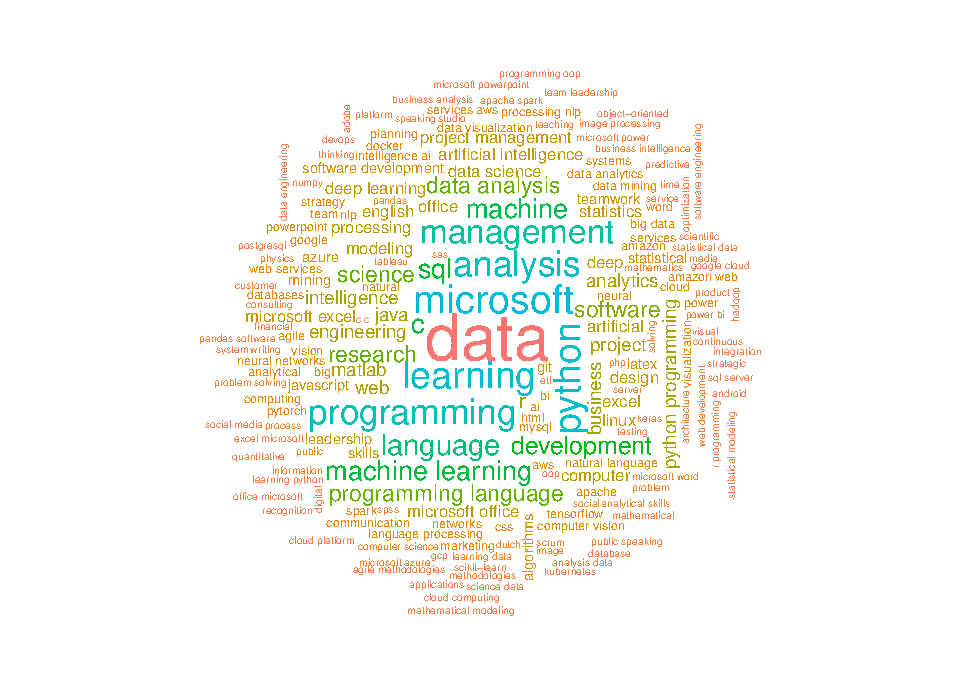
\includegraphics{figs/skill-wordcloud.pdf}

Among the most popular skills, Programming and Microsoft Office stand
out prominently. Additionally, programming languages like Python and SQL
show a significant presence, along with keywords such as Machine
Learning, Management, and Data Analysis. These skills and keywords
reflect their prevalence and importance in the current job market.

Next, the LDA algorithm is used with a specified number of topics to
uncover underlying themes or topics in the skill-related data. Here, we
experiment with number of topics being 3.

\begin{Shaded}
\begin{Highlighting}[]
\CommentTok{\# LDA {-} 3 topics}
\FunctionTok{set.seed}\NormalTok{(}\DecValTok{7}\NormalTok{)}
\NormalTok{lda\_skill\_3 }\OtherTok{\textless{}{-}} \FunctionTok{LDA}\NormalTok{(skill\_dtm, }\AttributeTok{method=}\StringTok{"Gibbs"}\NormalTok{, }\AttributeTok{k=}\DecValTok{3}\NormalTok{, }
                   \AttributeTok{control=}\FunctionTok{list}\NormalTok{(}\AttributeTok{iter =} \DecValTok{500}\NormalTok{, }\AttributeTok{verbose =} \DecValTok{25}\NormalTok{, }\AttributeTok{alpha =} \FloatTok{0.2}\NormalTok{))}
\end{Highlighting}
\end{Shaded}

\begin{verbatim}
## K = 3; V = 122909; M = 10977
## Sampling 500 iterations!
## Iteration 25 ...
## Iteration 50 ...
## Iteration 75 ...
## Iteration 100 ...
## Iteration 125 ...
## Iteration 150 ...
## Iteration 175 ...
## Iteration 200 ...
## Iteration 225 ...
## Iteration 250 ...
## Iteration 275 ...
## Iteration 300 ...
## Iteration 325 ...
## Iteration 350 ...
## Iteration 375 ...
## Iteration 400 ...
## Iteration 425 ...
## Iteration 450 ...
## Iteration 475 ...
## Iteration 500 ...
## Gibbs sampling completed!
\end{verbatim}

\begin{Shaded}
\begin{Highlighting}[]
\NormalTok{lda\_skill\_by\_3\_topics }\OtherTok{\textless{}{-}} \FunctionTok{tidy}\NormalTok{(lda\_skill\_3, }\AttributeTok{matrix =} \StringTok{"beta"}\NormalTok{)}

\NormalTok{lda\_skill\_by\_3\_topics }\OtherTok{\textless{}{-}}\NormalTok{ lda\_skill\_by\_3\_topics }\SpecialCharTok{\%\textgreater{}\%} 
  \FunctionTok{group\_by}\NormalTok{(topic) }\SpecialCharTok{\%\textgreater{}\%} 
  \FunctionTok{slice\_max}\NormalTok{(beta, }\AttributeTok{n =} \DecValTok{30}\NormalTok{) }\SpecialCharTok{\%\textgreater{}\%} 
  \FunctionTok{ungroup}\NormalTok{() }\SpecialCharTok{\%\textgreater{}\%} 
  \FunctionTok{arrange}\NormalTok{(topic, }\SpecialCharTok{{-}}\NormalTok{beta)}

\NormalTok{lda\_skill\_by\_3\_topics }\SpecialCharTok{\%\textgreater{}\%} 
  \FunctionTok{mutate}\NormalTok{(}\AttributeTok{term =} \FunctionTok{reorder\_within}\NormalTok{(term, beta, topic)) }\SpecialCharTok{\%\textgreater{}\%} 
  \FunctionTok{ggplot}\NormalTok{(}\FunctionTok{aes}\NormalTok{(beta, term, }\AttributeTok{fill =} \FunctionTok{factor}\NormalTok{(topic))) }\SpecialCharTok{+}
  \FunctionTok{geom\_col}\NormalTok{(}\AttributeTok{show.legend =} \ConstantTok{FALSE}\NormalTok{) }\SpecialCharTok{+}
  \FunctionTok{scale\_x\_continuous}\NormalTok{(}\AttributeTok{n.breaks =} \DecValTok{3}\NormalTok{) }\SpecialCharTok{+}
  \FunctionTok{facet\_wrap}\NormalTok{(}\SpecialCharTok{\textasciitilde{}}\NormalTok{ topic, }\AttributeTok{scales =} \StringTok{"free"}\NormalTok{, }\AttributeTok{ncol =} \DecValTok{4}\NormalTok{) }\SpecialCharTok{+}
  \FunctionTok{scale\_y\_reordered}\NormalTok{()}
\end{Highlighting}
\end{Shaded}

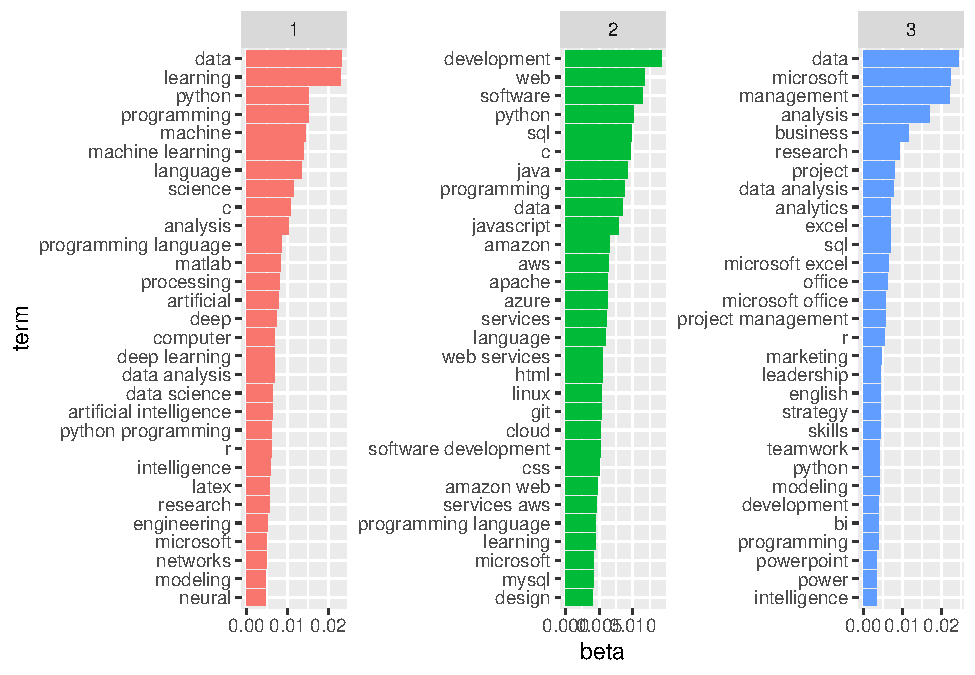
\includegraphics{figs/skill-lda-3.pdf}

The result yields three distinct topics, each characterized by a set of
relevant words that correspond to different skill sets required for
various positions. The interpretation of these topics is as follows:

\textbf{Topic 1}: Skills associated with a data scientist or machine
learning engineer role. \textbf{Topic 2}: Skills relevant to a data
engineer or software engineer role \textbf{Topic 3}: Skills commonly
expected in a business intelligence or data analyst role.

The analysis demonstrates a clear separation of skill sets, indicating
the effectiveness of the topic modeling process in identifying
meaningful clusters of skills. However, to enhance the feature
engineering task, we utilize the \texttt{ldatuning} package to determine
the optimal number of topics. By testing different topic numbers and
evaluating their performance using metrics like CaoJuan2009 and
Deveaud2014, we aim to strike the right balance between capturing
meaningful information and avoiding redundancy or noise. The tuning
process suggests that the ideal number of topics for our analysis is 8,
as indicated by both metrics.

\begin{Shaded}
\begin{Highlighting}[]
\CommentTok{\# Tuning}
\FunctionTok{set.seed}\NormalTok{(}\DecValTok{7}\NormalTok{)}
\NormalTok{result }\OtherTok{\textless{}{-}}\NormalTok{ ldatuning}\SpecialCharTok{::}\FunctionTok{FindTopicsNumber}\NormalTok{(}
\NormalTok{  skill\_dtm,}
  \AttributeTok{topics =} \FunctionTok{seq}\NormalTok{(}\AttributeTok{from =} \DecValTok{2}\NormalTok{, }\AttributeTok{to =} \DecValTok{10}\NormalTok{, }\AttributeTok{by =} \DecValTok{1}\NormalTok{),}
  \AttributeTok{metrics =} \FunctionTok{c}\NormalTok{(}\StringTok{"CaoJuan2009"}\NormalTok{,  }\StringTok{"Deveaud2014"}\NormalTok{),}
  \AttributeTok{method =} \StringTok{"Gibbs"}\NormalTok{,}
  \AttributeTok{control =} \FunctionTok{list}\NormalTok{(}\AttributeTok{iter =} \DecValTok{100}\NormalTok{, }\AttributeTok{verbose =} \DecValTok{25}\NormalTok{, }\AttributeTok{alpha =} \FloatTok{0.2}\NormalTok{),}
  \AttributeTok{verbose =} \ConstantTok{TRUE}
\NormalTok{)}
\end{Highlighting}
\end{Shaded}

\begin{verbatim}
## fit models... done.
## calculate metrics:
##   CaoJuan2009... done.
##   Deveaud2014... done.
\end{verbatim}

\begin{Shaded}
\begin{Highlighting}[]
\FunctionTok{FindTopicsNumber\_plot}\NormalTok{(result)}
\end{Highlighting}
\end{Shaded}

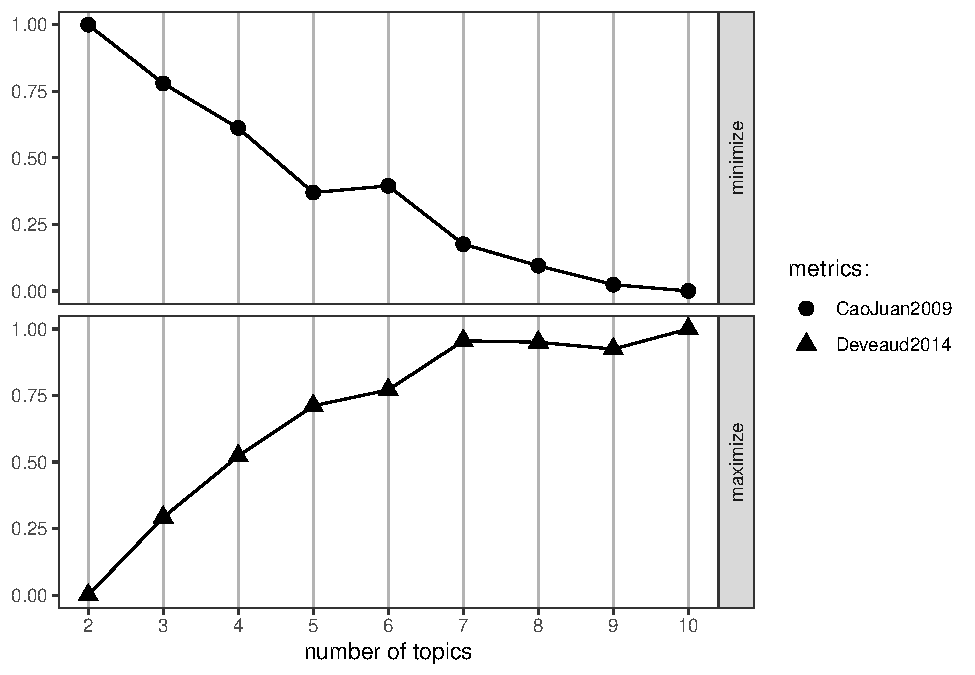
\includegraphics{figs/skill-tuning.pdf}

\begin{Shaded}
\begin{Highlighting}[]
\CommentTok{\# LDA {-} 8 topics}
\FunctionTok{set.seed}\NormalTok{(}\DecValTok{7}\NormalTok{)}
\NormalTok{lda\_skill\_8 }\OtherTok{\textless{}{-}} \FunctionTok{LDA}\NormalTok{(skill\_dtm, }\AttributeTok{method=}\StringTok{"Gibbs"}\NormalTok{, }\AttributeTok{k=}\DecValTok{8}\NormalTok{, }
                 \AttributeTok{control=}\FunctionTok{list}\NormalTok{(}\AttributeTok{iter =} \DecValTok{500}\NormalTok{, }\AttributeTok{verbose =} \DecValTok{25}\NormalTok{, }\AttributeTok{alpha =} \FloatTok{0.2}\NormalTok{))}
\end{Highlighting}
\end{Shaded}

\begin{verbatim}
## K = 8; V = 122909; M = 10977
## Sampling 500 iterations!
## Iteration 25 ...
## Iteration 50 ...
## Iteration 75 ...
## Iteration 100 ...
## Iteration 125 ...
## Iteration 150 ...
## Iteration 175 ...
## Iteration 200 ...
## Iteration 225 ...
## Iteration 250 ...
## Iteration 275 ...
## Iteration 300 ...
## Iteration 325 ...
## Iteration 350 ...
## Iteration 375 ...
## Iteration 400 ...
## Iteration 425 ...
## Iteration 450 ...
## Iteration 475 ...
## Iteration 500 ...
## Gibbs sampling completed!
\end{verbatim}

\begin{Shaded}
\begin{Highlighting}[]
\CommentTok{\# Visualization of most 30 most common terms}
\NormalTok{lda\_skill\_by\_8\_topics }\OtherTok{\textless{}{-}} \FunctionTok{tidy}\NormalTok{(lda\_skill\_8, }\AttributeTok{matrix =} \StringTok{"beta"}\NormalTok{)}
\NormalTok{lda\_skill\_by\_8\_topics }\OtherTok{\textless{}{-}}\NormalTok{ lda\_skill\_by\_8\_topics }\SpecialCharTok{\%\textgreater{}\%} 
  \FunctionTok{group\_by}\NormalTok{(topic) }\SpecialCharTok{\%\textgreater{}\%} 
  \FunctionTok{slice\_max}\NormalTok{(beta, }\AttributeTok{n =} \DecValTok{15}\NormalTok{) }\SpecialCharTok{\%\textgreater{}\%} 
  \FunctionTok{ungroup}\NormalTok{() }\SpecialCharTok{\%\textgreater{}\%} 
  \FunctionTok{arrange}\NormalTok{(topic, }\SpecialCharTok{{-}}\NormalTok{beta)}

\NormalTok{lda\_skill\_by\_8\_topics }\SpecialCharTok{\%\textgreater{}\%} 
  \FunctionTok{mutate}\NormalTok{(}\AttributeTok{term =} \FunctionTok{reorder\_within}\NormalTok{(term, beta, topic)) }\SpecialCharTok{\%\textgreater{}\%} 
  \FunctionTok{ggplot}\NormalTok{(}\FunctionTok{aes}\NormalTok{(beta, term, }\AttributeTok{fill =} \FunctionTok{factor}\NormalTok{(topic))) }\SpecialCharTok{+}
  \FunctionTok{geom\_col}\NormalTok{(}\AttributeTok{show.legend =} \ConstantTok{FALSE}\NormalTok{) }\SpecialCharTok{+}
  \FunctionTok{scale\_x\_continuous}\NormalTok{(}\AttributeTok{n.breaks =} \DecValTok{3}\NormalTok{) }\SpecialCharTok{+}
  \FunctionTok{facet\_wrap}\NormalTok{(}\SpecialCharTok{\textasciitilde{}}\NormalTok{ topic, }\AttributeTok{scales =} \StringTok{"free"}\NormalTok{, }\AttributeTok{ncol =} \DecValTok{4}\NormalTok{) }\SpecialCharTok{+}
  \FunctionTok{scale\_y\_reordered}\NormalTok{()}
\end{Highlighting}
\end{Shaded}

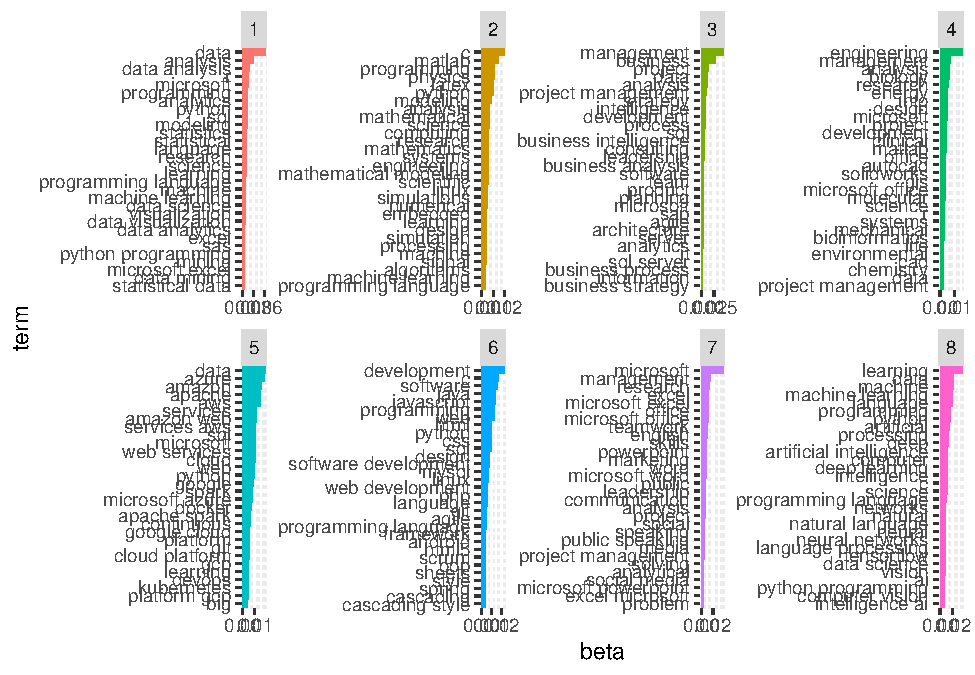
\includegraphics{figs/skill-lda-8.pdf}

Indeed, opting for 8 topics reveals a more nuanced and comprehensive
evaluation of the skills compared to the previous analysis. The
identified topics can be interpreted as follows:

\begin{itemize}
\tightlist
\item
  \textbf{Topic 1 (Data Analysis and Management)}: This topic seems to
  revolve around data analysis, data management, and related terms such
  as analytics and data visualization. It may cover skills and
  techniques used to explore and manage data efficiently.
\item
  \textbf{Topic 2 (Academic Tools and Programming Languages)}: This
  topic comprises terms associated with diverse programming languages
  like Python, MATLAB, and Latex, alongside indicators of tools and
  skills commonly employed in an academic setting, such as simulation,
  numerical analysis, and mathematical modeling.
\item
  \textbf{Topic 3 (Business Management and Strategy)}: This topic seems
  to be related to business management and strategy. It includes terms
  like project management, leadership, and teamwork, suggesting a focus
  on skills and knowledge related to business operations and
  decision-making.
\item
  \textbf{Topic 4 (Research and Scientific Analysis)}: This topic seems
  to be centered around research and scientific analysis. It includes
  terms like research, analysis, biology, and chemistry, suggesting a
  focus on scientific methods and data analysis in research settings.
\item
  \textbf{Topic 5 (Cloud Computing and Services)}: This topic appears to
  be related to cloud computing and services. It includes terms like AWS
  (Amazon Web Services), Azure, Google Cloud, and other web services,
  suggesting a focus on cloud-based technologies and services.
\item
  \textbf{Topic 6 (Programming Language and Web Development Tools)}:
  This topic seems to be related to tools commonly used by web and
  software developers, including programming languages like Java, HTML,
  PHP and CSS, along with management frameworks such as Agile and Scrum.
\item
  \textbf{Topic 7 (Office Productivity and Microsoft Tools)}: This topic
  is primarily centered around office productivity and Microsoft tools.
  It indicates proficiency in Microsoft productivity software and
  emphasizes soft skills like communication, public speaking, and
  project management.
\item
  \textbf{Topic 8 (Artificial Intelligence and Machine Learning)}: This
  topic revolves around artificial intelligence (AI) and machine
  learning (ML). It incorporates terms like machine learning, deep
  learning, artificial intelligence, and natural language processing,
  indicating a strong emphasis on AI and ML technologies and their
  applications.
\end{itemize}

\begin{Shaded}
\begin{Highlighting}[]
\CommentTok{\# Get the topic distributions for each line in skill dataframe}
\NormalTok{topic\_dist\_8 }\OtherTok{\textless{}{-}} \FunctionTok{as.data.frame}\NormalTok{(}\FunctionTok{posterior}\NormalTok{(lda\_skill\_8)}\SpecialCharTok{$}\NormalTok{topics)}
\NormalTok{topic\_dist\_3 }\OtherTok{\textless{}{-}} \FunctionTok{as.data.frame}\NormalTok{(}\FunctionTok{posterior}\NormalTok{(lda\_skill\_3)}\SpecialCharTok{$}\NormalTok{topics)}

\CommentTok{\# Determine the strongest role using LDA with 3 topics}
\NormalTok{strongest\_role }\OtherTok{\textless{}{-}} \FunctionTok{topics}\NormalTok{(lda\_skill\_3)}

\CommentTok{\# Combine the topic distribution and strongest role with the original skill dataframe}
\NormalTok{skill\_topic\_df }\OtherTok{\textless{}{-}} \FunctionTok{cbind}\NormalTok{(skill, topic\_dist\_8, strongest\_role) }\SpecialCharTok{\%\textgreater{}\%}
  \FunctionTok{rename}\NormalTok{(}\StringTok{"skill1"}\OtherTok{=}\StringTok{"1"}\NormalTok{, }\StringTok{"skill2"}\OtherTok{=}\StringTok{"2"}\NormalTok{, }\StringTok{"skill3"}\OtherTok{=}\StringTok{"3"}\NormalTok{,}
         \StringTok{"skill4"}\OtherTok{=}\StringTok{"4"}\NormalTok{, }\StringTok{"skill5"}\OtherTok{=}\StringTok{"5"}\NormalTok{, }\StringTok{"skill6"}\OtherTok{=}\StringTok{"6"}\NormalTok{,}
         \StringTok{"skill7"}\OtherTok{=}\StringTok{"7"}\NormalTok{, }\StringTok{"skill8"}\OtherTok{=}\StringTok{"8"}\NormalTok{)}

\CommentTok{\# Set topic distribution columns to 0 and strongest\_role to NA where skills is NA}
\NormalTok{skill\_topic\_df[}\FunctionTok{is.na}\NormalTok{(skill\_topic\_df}\SpecialCharTok{$}\NormalTok{skills), }\DecValTok{4}\SpecialCharTok{:}\DecValTok{11}\NormalTok{] }\OtherTok{\textless{}{-}} \DecValTok{0}
\NormalTok{skill\_topic\_df[}\FunctionTok{is.na}\NormalTok{(skill\_topic\_df}\SpecialCharTok{$}\NormalTok{skills), }\DecValTok{12}\NormalTok{] }\OtherTok{\textless{}{-}} \ConstantTok{NA}

\NormalTok{knitr}\SpecialCharTok{::}\FunctionTok{kable}\NormalTok{(}\FunctionTok{head}\NormalTok{(skill\_topic\_df, }\DecValTok{5}\NormalTok{))}

\FunctionTok{write.csv}\NormalTok{(skill\_topic\_df, }\StringTok{"skill\_processed.csv"}\NormalTok{, }\AttributeTok{row.names =} \ConstantTok{FALSE}\NormalTok{)}
\end{Highlighting}
\end{Shaded}

From the topic modeling process using Latent Dirichlet Allocation (LDA)
with 8 topics, we have extracted the topic distribution for each entry
in the \texttt{skill} dataframe. This resulting dataframe will show the
probabilities of each individual's skills belonging to each of the 8
skill topics and will be saved for future analysis. Additionally, we
determined the strongest role of each person based on the topic modeling
results with 3 topics.

\begin{Shaded}
\begin{Highlighting}[]
\NormalTok{skill\_topic\_df\_full }\OtherTok{\textless{}{-}} \FunctionTok{cbind}\NormalTok{(skill\_topic\_df, topic\_dist\_3) }\SpecialCharTok{\%\textgreater{}\%} 
  \FunctionTok{rename}\NormalTok{(}\StringTok{"role1"}\OtherTok{=}\StringTok{"1"}\NormalTok{, }\StringTok{"role2"}\OtherTok{=}\StringTok{"2"}\NormalTok{, }\StringTok{"role3"}\OtherTok{=}\StringTok{"3"}\NormalTok{)}

\NormalTok{skill\_topic\_df\_full[}\FunctionTok{is.na}\NormalTok{(skill\_topic\_df\_full}\SpecialCharTok{$}\NormalTok{skills), }\DecValTok{4}\SpecialCharTok{:}\DecValTok{11}\NormalTok{] }\OtherTok{\textless{}{-}} \DecValTok{0}
\NormalTok{skill\_topic\_df\_full[}\FunctionTok{is.na}\NormalTok{(skill\_topic\_df\_full}\SpecialCharTok{$}\NormalTok{skills), }\DecValTok{13}\SpecialCharTok{:}\DecValTok{15}\NormalTok{] }\OtherTok{\textless{}{-}} \DecValTok{0}
\NormalTok{skill\_topic\_df\_full[}\FunctionTok{is.na}\NormalTok{(skill\_topic\_df\_full}\SpecialCharTok{$}\NormalTok{skills), }\DecValTok{12}\NormalTok{] }\OtherTok{\textless{}{-}} \ConstantTok{NA}

\CommentTok{\# List of skill{-}related numerical variables}
\NormalTok{skill\_related\_vars }\OtherTok{\textless{}{-}} \FunctionTok{c}\NormalTok{(}\StringTok{"skill1"}\NormalTok{, }\StringTok{"skill2"}\NormalTok{, }\StringTok{"skill3"}\NormalTok{, }\StringTok{"skill5"}\NormalTok{, }
                        \StringTok{"skill6"}\NormalTok{, }\StringTok{"skill7"}\NormalTok{, }\StringTok{"skill8"}\NormalTok{)}

\CommentTok{\# List of role{-}related numerical variables (excluding "strongest\_role")}
\NormalTok{role\_related\_vars }\OtherTok{\textless{}{-}} \FunctionTok{c}\NormalTok{(}\StringTok{"role1"}\NormalTok{, }\StringTok{"role2"}\NormalTok{, }\StringTok{"role3"}\NormalTok{)}

\CommentTok{\# Calculate the Pearson correlation between skill{-}related and role{-}related variables}
\NormalTok{cor\_results }\OtherTok{\textless{}{-}} \FunctionTok{cor}\NormalTok{(skill\_topic\_df\_full[, skill\_related\_vars], }
\NormalTok{                   skill\_topic\_df\_full[, role\_related\_vars], }\AttributeTok{method =} \StringTok{"pearson"}\NormalTok{)}

\CommentTok{\# Print the correlation results}
\FunctionTok{print}\NormalTok{(cor\_results)}
\end{Highlighting}
\end{Shaded}

To reaffirm our understanding of skills and roles in the context of our
study, we conducted a Pearson correlation analysis between skill-related
and role-related variables. The results indicate clear patterns:

\textbf{Role 1 (Data Scientist/ML Engineer)} shows the highest positive
correlation with skill8 and skill2. These skills encompass AI/ML tools,
mathematical and programming tools commonly used in an academic setting.

\textbf{Role 2 (Data/Software Engineer)} is most positively correlated
with skill6 and skill5. These skills cover programming languages, web
development, and cloud computing services, which are essential in this
role.

\textbf{Role 3 (BI/Data Analyst)} exhibits the strongest positive
correlation with skill7 and skill3. These skills revolve around business
strategy, soft skills, and office productivity, aligning well with the
responsibilities of a BI/Data Analyst.

Overall, the observed correlations align with the established norms in
the data science and IT field, further supporting our interpretations of
the relationship between skills and roles.

\hypertarget{exploratory-data-analysis}{%
\section{Exploratory Data Analysis}\label{exploratory-data-analysis}}

\hypertarget{the-most-common-industries}{%
\subsection{The most common
industries}\label{the-most-common-industries}}

First and foremost, the most common industries among employees are
identified. In the following code, a \texttt{industry\_counts} variable
is created, which holds the counts of employees in each industry. To
present this information in a more visually appealing manner, a word
cloud is generated, highlighting the top 30 industries based on their
frequencies respectively.

\begin{Shaded}
\begin{Highlighting}[]
\NormalTok{industry\_counts }\OtherTok{\textless{}{-}}\NormalTok{ exp }\SpecialCharTok{\%\textgreater{}\%}
  \FunctionTok{group\_by}\NormalTok{(employee\_id, industry) }\SpecialCharTok{\%\textgreater{}\%}
  \FunctionTok{summarise}\NormalTok{(}\AttributeTok{count =} \FunctionTok{n\_distinct}\NormalTok{(industry)) }\SpecialCharTok{\%\textgreater{}\%}
  \FunctionTok{group\_by}\NormalTok{(industry) }\SpecialCharTok{\%\textgreater{}\%}
  \FunctionTok{count}\NormalTok{() }\SpecialCharTok{\%\textgreater{}\%}
  \FunctionTok{arrange}\NormalTok{(}\FunctionTok{desc}\NormalTok{(n))}

\FunctionTok{wordcloud}\NormalTok{(}\AttributeTok{words =}\NormalTok{ industry\_counts}\SpecialCharTok{$}\NormalTok{industry[}\DecValTok{1}\SpecialCharTok{:}\DecValTok{30}\NormalTok{], }\AttributeTok{freq =}\NormalTok{ industry\_counts}\SpecialCharTok{$}\NormalTok{n[}\DecValTok{1}\SpecialCharTok{:}\DecValTok{30}\NormalTok{],}
          \AttributeTok{scale =} \FunctionTok{c}\NormalTok{(}\DecValTok{1}\NormalTok{, }\FloatTok{0.5}\NormalTok{), }\AttributeTok{random.order =} \ConstantTok{FALSE}\NormalTok{,}
          \AttributeTok{colors =} \FunctionTok{brewer.pal}\NormalTok{(}\DecValTok{8}\NormalTok{, }\StringTok{"Set2"}\NormalTok{), }\AttributeTok{min.freq =} \DecValTok{1}\NormalTok{)}
\end{Highlighting}
\end{Shaded}

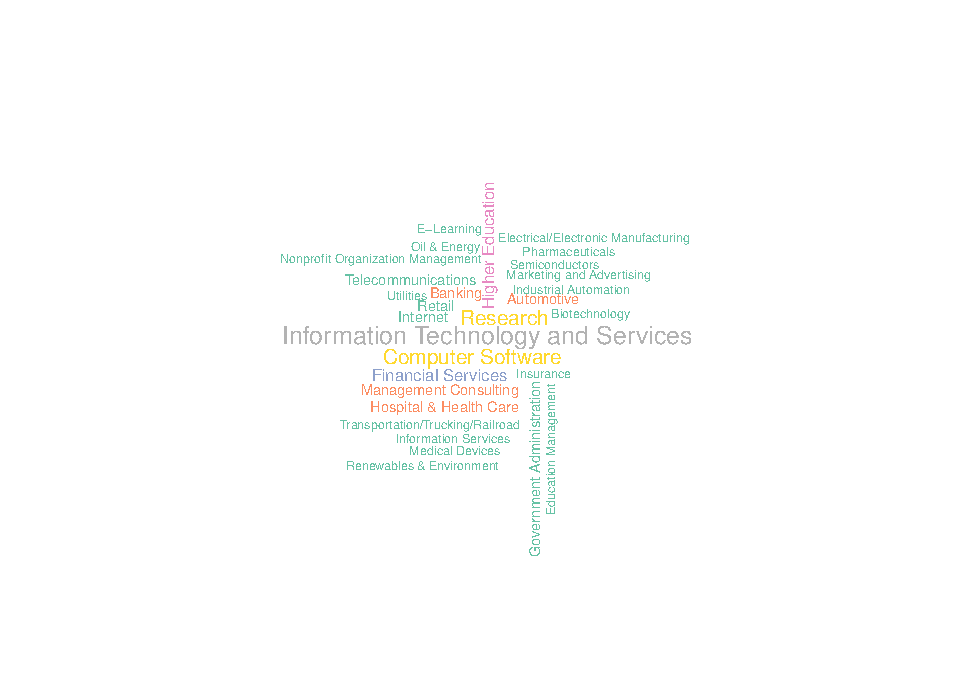
\includegraphics{figs/eda-industry-wordcloud.pdf}

As data science and AI fields are highly associated with information
technology, it's not surprising to see that the most frequent industry
is Information Technology and Services, which is followed by Computer
Software, Research and so forth. It's also interesting to notice that
the list reflects a diverse range of industries, including Banking,
Healthcare, Automotive, Telecommunications, and more, indicating the
versatility and applicability of data science and AI across various
sectors.

\begin{Shaded}
\begin{Highlighting}[]
\CommentTok{\# Display the table of most common industries}
\NormalTok{top\_industries\_table }\OtherTok{\textless{}{-}}\NormalTok{ industry\_counts }\SpecialCharTok{\%\textgreater{}\%}
  \FunctionTok{head}\NormalTok{(}\DecValTok{30}\NormalTok{)}
\NormalTok{top\_industries\_table}
\end{Highlighting}
\end{Shaded}

\begin{verbatim}
## # A tibble: 30 x 2
## # Groups:   industry [30]
##    industry                                n
##    <chr>                               <int>
##  1 Information Technology and Services  5018
##  2 Computer Software                    3670
##  3 <NA>                                 3240
##  4 Research                             3159
##  5 Higher Education                     2065
##  6 Financial Services                   1427
##  7 Management Consulting                1152
##  8 Banking                               821
##  9 Hospital & Health Care                772
## 10 Automotive                            668
## # i 20 more rows
\end{verbatim}

\hypertarget{the-most-common-job-titles}{%
\subsection{The most common job
titles}\label{the-most-common-job-titles}}

This process aims to reveal recurring word combinations within job
titles and extract the most frequent bi-grams and tri-grams.

\begin{Shaded}
\begin{Highlighting}[]
\CommentTok{\# Preprocess the title data}
\CommentTok{\# Filter out NA values in the "title" column}
\NormalTok{title\_data }\OtherTok{\textless{}{-}}\NormalTok{ exp }\SpecialCharTok{\%\textgreater{}\%}
  \FunctionTok{filter}\NormalTok{(}\SpecialCharTok{!}\FunctionTok{is.na}\NormalTok{(title))}

\CommentTok{\# Preprocess the title data for bi{-}grams}
\NormalTok{bigrams }\OtherTok{\textless{}{-}}\NormalTok{ title\_data }\SpecialCharTok{\%\textgreater{}\%}
\NormalTok{  dplyr}\SpecialCharTok{::}\FunctionTok{select}\NormalTok{(title) }\SpecialCharTok{\%\textgreater{}\%}
  \FunctionTok{mutate}\NormalTok{(}\AttributeTok{title =} \FunctionTok{tolower}\NormalTok{(title)) }\SpecialCharTok{\%\textgreater{}\%}
  \FunctionTok{unnest\_tokens}\NormalTok{(}\AttributeTok{input =}\NormalTok{ title, }\AttributeTok{output =} \StringTok{"tokens"}\NormalTok{, }\AttributeTok{token =} \StringTok{"ngrams"}\NormalTok{, }\AttributeTok{n =} \DecValTok{2}\NormalTok{) }\SpecialCharTok{\%\textgreater{}\%}
  \FunctionTok{mutate}\NormalTok{(}\AttributeTok{tokens =} \FunctionTok{str\_replace\_all}\NormalTok{(tokens, }\StringTok{"[\^{}[:alnum:]}\SpecialCharTok{\textbackslash{}\textbackslash{}}\StringTok{s]"}\NormalTok{, }\StringTok{""}\NormalTok{))}

\NormalTok{trigrams }\OtherTok{\textless{}{-}}\NormalTok{ title\_data }\SpecialCharTok{\%\textgreater{}\%}
\NormalTok{  dplyr}\SpecialCharTok{::}\FunctionTok{select}\NormalTok{(title) }\SpecialCharTok{\%\textgreater{}\%}
  \FunctionTok{mutate}\NormalTok{(}\AttributeTok{title =} \FunctionTok{tolower}\NormalTok{(title)) }\SpecialCharTok{\%\textgreater{}\%}
  \FunctionTok{unnest\_tokens}\NormalTok{(}\AttributeTok{input =}\NormalTok{ title, }\AttributeTok{output =} \StringTok{"tokens"}\NormalTok{, }\AttributeTok{token =} \StringTok{"ngrams"}\NormalTok{, }\AttributeTok{n =} \DecValTok{3}\NormalTok{) }\SpecialCharTok{\%\textgreater{}\%}
  \FunctionTok{mutate}\NormalTok{(}\AttributeTok{tokens =} \FunctionTok{str\_replace\_all}\NormalTok{(tokens, }\StringTok{"[\^{}[:alnum:]}\SpecialCharTok{\textbackslash{}\textbackslash{}}\StringTok{s]"}\NormalTok{, }\StringTok{""}\NormalTok{))}

\CommentTok{\# Load stopwords and additional custom words to remove}
\NormalTok{stop\_words }\OtherTok{\textless{}{-}} \FunctionTok{bind\_rows}\NormalTok{(}\FunctionTok{list}\NormalTok{(}\FunctionTok{data.frame}\NormalTok{(}\AttributeTok{word =} \FunctionTok{stopwords}\NormalTok{(}\StringTok{"en"}\NormalTok{), }
                                        \AttributeTok{stringsAsFactors =} \ConstantTok{FALSE}\NormalTok{),}
                             \FunctionTok{data.frame}\NormalTok{(}\AttributeTok{word =} \FunctionTok{c}\NormalTok{(}\StringTok{"title"}\NormalTok{), }
                                        \AttributeTok{stringsAsFactors =} \ConstantTok{FALSE}\NormalTok{)))}

\CommentTok{\# Remove stop words}
\NormalTok{bigram\_processed }\OtherTok{\textless{}{-}}\NormalTok{ bigrams }\SpecialCharTok{\%\textgreater{}\%}
  \FunctionTok{anti\_join}\NormalTok{(stop\_words, }\AttributeTok{by =} \FunctionTok{c}\NormalTok{(}\StringTok{"tokens"} \OtherTok{=} \StringTok{"word"}\NormalTok{))}
\NormalTok{trigram\_processed }\OtherTok{\textless{}{-}}\NormalTok{ trigrams }\SpecialCharTok{\%\textgreater{}\%}
  \FunctionTok{anti\_join}\NormalTok{(stop\_words, }\AttributeTok{by =} \FunctionTok{c}\NormalTok{(}\StringTok{"tokens"} \OtherTok{=} \StringTok{"word"}\NormalTok{))}

\CommentTok{\# Find the most frequent titles}
\NormalTok{top\_bigram\_titles }\OtherTok{\textless{}{-}}\NormalTok{ bigram\_processed }\SpecialCharTok{\%\textgreater{}\%}
  \FunctionTok{count}\NormalTok{(tokens, }\AttributeTok{sort =} \ConstantTok{TRUE}\NormalTok{) }\SpecialCharTok{\%\textgreater{}\%}
  \FunctionTok{top\_n}\NormalTok{(}\DecValTok{40}\NormalTok{)}

\NormalTok{top\_trigram\_titles }\OtherTok{\textless{}{-}}\NormalTok{ trigram\_processed }\SpecialCharTok{\%\textgreater{}\%}
  \FunctionTok{count}\NormalTok{(tokens, }\AttributeTok{sort =} \ConstantTok{TRUE}\NormalTok{) }\SpecialCharTok{\%\textgreater{}\%}
  \FunctionTok{top\_n}\NormalTok{(}\DecValTok{40}\NormalTok{)}

\CommentTok{\# Print the most frequent titles}
\FunctionTok{print}\NormalTok{(top\_bigram\_titles)}
\end{Highlighting}
\end{Shaded}

\begin{verbatim}
## # A tibble: 40 x 2
##    tokens                 n
##    <chr>              <int>
##  1 data scientist      5209
##  2 <NA>                3774
##  3 machine learning    3042
##  4 software engineer   2544
##  5 data engineer       2016
##  6 learning engineer   1968
##  7 data analyst        1630
##  8 data science        1394
##  9 senior data         1018
## 10 research assistant   930
## # i 30 more rows
\end{verbatim}

\begin{Shaded}
\begin{Highlighting}[]
\FunctionTok{print}\NormalTok{(top\_trigram\_titles)}
\end{Highlighting}
\end{Shaded}

\begin{verbatim}
## # A tibble: 40 x 2
##    tokens                        n
##    <chr>                     <int>
##  1 <NA>                      22320
##  2 machine learning engineer  1890
##  3 senior data scientist       634
##  4 senior software engineer    351
##  5 senior machine learning     248
##  6 data science intern         242
##  7 lead data scientist         222
##  8 full stack developer        215
##  9 master thesis student       183
## 10 senior data engineer        178
## # i 30 more rows
\end{verbatim}

Notably, ``Data Scientist'' emerges as the most prevalent job title,
with a frequency of 5209 occurrences, which is followed by ``Machine
Learning'', ``Software Engineer'', ``Data Engineer'', and so on.
Moreover, the dataset highlights the importance of senior-level
positions within various domains. It reveals the prevalence of ``Senior
Data'' and ``Senior Machine Learning'' positions, indicating significant
roles held by experienced professionals in data and machine learning
fields, respectively. Overall, the dataset centers on data science,
machine learning, and software-related roles, with an emphasis on
senior-level positions.

\hypertarget{modelling}{%
\subsection{Modelling}\label{modelling}}

\begin{Shaded}
\begin{Highlighting}[]
\CommentTok{\# Load data}
\NormalTok{gender\_data }\OtherTok{=} \FunctionTok{read\_csv}\NormalTok{(}\FunctionTok{paste}\NormalTok{(}\StringTok{"https://raw.githubusercontent.com/tiendd712/"}\NormalTok{,}
                        \StringTok{"Socialscience\_bigdata\_KUL/master/Assignment\%203/"}\NormalTok{,}
                        \StringTok{"data\_processing/final\_processed\_data/gender\_processed.csv"}\NormalTok{,}
                        \AttributeTok{sep =} \StringTok{""}\NormalTok{)) }\SpecialCharTok{\%\textgreater{}\%}\NormalTok{ dplyr}\SpecialCharTok{::}\FunctionTok{select}\NormalTok{(employee\_id, gender\_predict)}



\NormalTok{edu\_data }\OtherTok{=} \FunctionTok{read\_csv}\NormalTok{(}\FunctionTok{paste}\NormalTok{(}\StringTok{"https://raw.githubusercontent.com/tiendd712/"}\NormalTok{,}
                        \StringTok{"Socialscience\_bigdata\_KUL/master/Assignment\%203/"}\NormalTok{,}
                        \StringTok{"data\_processing/final\_processed\_data/edu\_processed.csv"}\NormalTok{,}
                        \AttributeTok{sep =} \StringTok{""}\NormalTok{)) }

\NormalTok{lang\_data }\OtherTok{=} \FunctionTok{read\_csv}\NormalTok{(}\FunctionTok{paste}\NormalTok{(}\StringTok{"https://raw.githubusercontent.com/tiendd712/"}\NormalTok{,}
                        \StringTok{"Socialscience\_bigdata\_KUL/master/Assignment\%203/"}\NormalTok{,}
                        \StringTok{"data\_processing/final\_processed\_data/lang\_processed.csv"}\NormalTok{,}
                        \AttributeTok{sep =} \StringTok{""}\NormalTok{)) }

\NormalTok{follower\_data }\OtherTok{=} \FunctionTok{read\_csv}\NormalTok{(}\FunctionTok{paste}\NormalTok{(}\StringTok{"https://raw.githubusercontent.com/tiendd712/"}\NormalTok{,}
                        \StringTok{"Socialscience\_bigdata\_KUL/master/Assignment\%203/"}\NormalTok{,}
                        \StringTok{"data\_processing/follower\_data.csv"}\NormalTok{,}
                        \AttributeTok{sep =} \StringTok{""}\NormalTok{)) }

\NormalTok{connection\_data }\OtherTok{=} \FunctionTok{read\_csv}\NormalTok{(}\FunctionTok{paste}\NormalTok{(}\StringTok{"https://raw.githubusercontent.com/tiendd712/"}\NormalTok{,}
                        \StringTok{"Socialscience\_bigdata\_KUL/master/Assignment\%203/"}\NormalTok{,}
                        \StringTok{"data\_processing/connection\_data.csv"}\NormalTok{,}
                        \AttributeTok{sep =} \StringTok{""}\NormalTok{)) }

\NormalTok{skill\_data }\OtherTok{=} \FunctionTok{read\_csv}\NormalTok{(}\FunctionTok{paste}\NormalTok{(}\StringTok{"https://raw.githubusercontent.com/tiendd712/"}\NormalTok{,}
                        \StringTok{"Socialscience\_bigdata\_KUL/master/Assignment\%203/"}\NormalTok{,}
                        \StringTok{"data\_processing/final\_processed\_data/skill\_processed.csv"}\NormalTok{,}
                        \AttributeTok{sep =} \StringTok{""}\NormalTok{)) }

\NormalTok{exp\_data }\OtherTok{=} \FunctionTok{read\_csv}\NormalTok{(}\FunctionTok{paste}\NormalTok{(}\StringTok{"https://raw.githubusercontent.com/tiendd712/"}\NormalTok{,}
                        \StringTok{"Socialscience\_bigdata\_KUL/master/Assignment\%203/"}\NormalTok{,}
                        \StringTok{"data\_processing/final\_processed\_data/exp\_processed.csv"}\NormalTok{,}
                        \AttributeTok{sep =} \StringTok{""}\NormalTok{)) }

\NormalTok{language\_columns }\OtherTok{\textless{}{-}} \FunctionTok{c}\NormalTok{(}\StringTok{"English"}\NormalTok{, }\StringTok{"French"}\NormalTok{, }\StringTok{"Dutch"}\NormalTok{, }\StringTok{"German"}\NormalTok{, }
                      \StringTok{"Spanish"}\NormalTok{, }\StringTok{"Hindi"}\NormalTok{, }\StringTok{"Chinese"}\NormalTok{)}
\end{Highlighting}
\end{Shaded}

\hypertarget{what-factors-are-significantly-associated-with-the-probability-of-receiving-promotions-in-the-data-science-it-software-and-artificial-intelligence-fields}{%
\subsection{What factors are significantly associated with the
probability of receiving promotions in the data science, IT, software,
and artificial intelligence
fields?}\label{what-factors-are-significantly-associated-with-the-probability-of-receiving-promotions-in-the-data-science-it-software-and-artificial-intelligence-fields}}

We implement a Logistic Regression model and XGboost model to analyze
the association between various features and the likelihood of employee
promotions.

Firstly, several datasets are merged into a comprehensive dataset by the
\texttt{employee\_id}. We filtered to get records where
\texttt{time\_work} is greater than 0 and some variables are transformed
to appropriate data types. The data is split into training and testing
sets, with the ratio of 80:20.

In the section, we present the models that predict the probability of
getting promoted to level 1 position (job titles containing keywords
such as \texttt{lead}, \texttt{senior}, \texttt{sr}, and
\texttt{principal}) and the probability of getting promoted to either
level 1 or level 2 (also incorporating keywords like \texttt{head},
\texttt{supervisor}, \texttt{manager}, \texttt{director}, and
\texttt{expert}).

Regarding the model predict the probability of getting promoted to level
1 position, we noticed that certain individuals bypass the level 1
position and are directly promoted to level 2 positions. In order to
correctly classify these people who get promoted, we have excluded these
cases from our models.

\begin{Shaded}
\begin{Highlighting}[]
\CommentTok{\# Model promoted to level 1}
\DocumentationTok{\#\# Preprocess the data}
\NormalTok{df }\OtherTok{=}\NormalTok{ exp\_data }\SpecialCharTok{\%\textgreater{}\%}
  \FunctionTok{merge}\NormalTok{(edu\_data, }\AttributeTok{by =} \StringTok{"employee\_id"}\NormalTok{, }\AttributeTok{all.x =} \ConstantTok{TRUE}\NormalTok{) }\SpecialCharTok{\%\textgreater{}\%}
  \FunctionTok{filter}\NormalTok{(time\_work }\SpecialCharTok{\textgreater{}} \DecValTok{0}\NormalTok{) }\SpecialCharTok{\%\textgreater{}\%} 
  \FunctionTok{merge}\NormalTok{(lang\_data, }\AttributeTok{by =} \StringTok{"employee\_id"}\NormalTok{, }\AttributeTok{all.x =} \ConstantTok{TRUE}\NormalTok{) }\SpecialCharTok{\%\textgreater{}\%}
  \FunctionTok{merge}\NormalTok{(connection\_data, }\AttributeTok{by =} \StringTok{"employee\_id"}\NormalTok{, }\AttributeTok{all.x =} \ConstantTok{TRUE}\NormalTok{) }\SpecialCharTok{\%\textgreater{}\%}
  \FunctionTok{merge}\NormalTok{(follower\_data, }\AttributeTok{by =} \StringTok{"employee\_id"}\NormalTok{, }\AttributeTok{all.x =} \ConstantTok{TRUE}\NormalTok{) }\SpecialCharTok{\%\textgreater{}\%}
  \FunctionTok{merge}\NormalTok{(skill\_data, }\AttributeTok{by =} \StringTok{"employee\_id"}\NormalTok{, }\AttributeTok{all.x =} \ConstantTok{TRUE}\NormalTok{) }\SpecialCharTok{\%\textgreater{}\%} 
  \FunctionTok{merge}\NormalTok{(gender\_data, }\AttributeTok{by =} \StringTok{"employee\_id"}\NormalTok{, }\AttributeTok{all.x =} \ConstantTok{TRUE}\NormalTok{) }\SpecialCharTok{\%\textgreater{}\%} 
\NormalTok{  dplyr}\SpecialCharTok{::}\FunctionTok{select}\NormalTok{(}\SpecialCharTok{{-}}\NormalTok{skills, }\SpecialCharTok{{-}}\NormalTok{skill\_trans, }\SpecialCharTok{{-}}\NormalTok{strongest\_role, }\SpecialCharTok{{-}}\NormalTok{skill4, }\SpecialCharTok{{-}}\NormalTok{last\_edu\_year,}
                \SpecialCharTok{{-}}\NormalTok{connection\_count, }\SpecialCharTok{{-}}\NormalTok{employee\_id) }\SpecialCharTok{\%\textgreater{}\%}
  \FunctionTok{mutate}\NormalTok{(}\AttributeTok{gender\_predict =} \FunctionTok{ifelse}\NormalTok{(}\FunctionTok{is.na}\NormalTok{(gender\_predict), }\StringTok{"Neutral"}\NormalTok{, gender\_predict)) }\SpecialCharTok{\%\textgreater{}\%}
  \FunctionTok{mutate}\NormalTok{(}\AttributeTok{promote\_level\_1 =} \FunctionTok{ifelse}\NormalTok{(}\FunctionTok{is.na}\NormalTok{(promote\_level\_1), }\DecValTok{0}\NormalTok{, promote\_level\_1)) }\SpecialCharTok{\%\textgreater{}\%}
  \FunctionTok{mutate}\NormalTok{(}\AttributeTok{highest\_edu =} \FunctionTok{ifelse}\NormalTok{(}\FunctionTok{is.na}\NormalTok{(highest\_edu), }\StringTok{"bachelor"}\NormalTok{, highest\_edu)) }\SpecialCharTok{\%\textgreater{}\%}
  \FunctionTok{replace}\NormalTok{(}\FunctionTok{is.na}\NormalTok{(.), }\DecValTok{0}\NormalTok{) }\SpecialCharTok{\%\textgreater{}\%}
  \FunctionTok{mutate}\NormalTok{(}\AttributeTok{promote\_level\_1 =} \FunctionTok{factor}\NormalTok{(promote\_level\_1, }
                                  \AttributeTok{levels =} \FunctionTok{c}\NormalTok{(}\DecValTok{0}\NormalTok{, }\DecValTok{1}\NormalTok{), }
                                  \AttributeTok{labels =} \FunctionTok{c}\NormalTok{(}\DecValTok{0}\NormalTok{, }\DecValTok{1}\NormalTok{)),}
         \AttributeTok{gender\_predict =} \FunctionTok{factor}\NormalTok{(gender\_predict, }
                                 \AttributeTok{levels =} \FunctionTok{c}\NormalTok{(}\StringTok{"Man"}\NormalTok{, }\StringTok{"Woman"}\NormalTok{, }\StringTok{"Neutral"}\NormalTok{), }
                                 \AttributeTok{labels =} \FunctionTok{c}\NormalTok{(}\DecValTok{0}\NormalTok{, }\DecValTok{1}\NormalTok{, }\DecValTok{2}\NormalTok{)),}
         \AttributeTok{highest\_edu =} \FunctionTok{factor}\NormalTok{(highest\_edu, }
                              \AttributeTok{levels =} \FunctionTok{c}\NormalTok{(}\StringTok{"bachelor"}\NormalTok{, }\StringTok{"master"}\NormalTok{, }\StringTok{"phd"}\NormalTok{), }
                              \AttributeTok{labels =} \FunctionTok{c}\NormalTok{(}\DecValTok{0}\NormalTok{, }\DecValTok{1}\NormalTok{, }\DecValTok{2}\NormalTok{)),}
         \AttributeTok{has\_relevant\_field =} \FunctionTok{factor}\NormalTok{(has\_relevant\_field, }
                                     \AttributeTok{levels =} \FunctionTok{c}\NormalTok{(}\DecValTok{0}\NormalTok{, }\DecValTok{1}\NormalTok{), }
                                     \AttributeTok{labels =} \FunctionTok{c}\NormalTok{(}\DecValTok{0}\NormalTok{, }\DecValTok{1}\NormalTok{)),}
         \AttributeTok{intern =} \FunctionTok{factor}\NormalTok{(intern, }
                         \AttributeTok{levels =} \FunctionTok{c}\NormalTok{(}\DecValTok{0}\NormalTok{, }\DecValTok{1}\NormalTok{), }
                         \AttributeTok{labels =} \FunctionTok{c}\NormalTok{(}\DecValTok{0}\NormalTok{, }\DecValTok{1}\NormalTok{)),}
         \AttributeTok{connection\_type =} \FunctionTok{factor}\NormalTok{(connection\_type, }
                                  \AttributeTok{levels =} \FunctionTok{c}\NormalTok{(}\DecValTok{0}\NormalTok{, }\DecValTok{1}\NormalTok{), }
                                  \AttributeTok{labels =} \FunctionTok{c}\NormalTok{(}\DecValTok{0}\NormalTok{, }\DecValTok{1}\NormalTok{))) }\SpecialCharTok{\%\textgreater{}\%} 
  \FunctionTok{mutate\_at}\NormalTok{(}\FunctionTok{vars}\NormalTok{(}\FunctionTok{all\_of}\NormalTok{(language\_columns)), factor,}
            \AttributeTok{levels =} \FunctionTok{c}\NormalTok{(}\DecValTok{0}\NormalTok{, }\DecValTok{1}\NormalTok{))}

\NormalTok{df\_level\_1 }\OtherTok{=}\NormalTok{ df }\SpecialCharTok{\%\textgreater{}\%} \FunctionTok{filter}\NormalTok{(}\SpecialCharTok{!}\NormalTok{(promote\_level\_1 }\SpecialCharTok{==}  \DecValTok{0} \SpecialCharTok{\&}\NormalTok{ promote\_level\_2 }\SpecialCharTok{==} \DecValTok{1}\NormalTok{)) }

\FunctionTok{kable\_styling}\NormalTok{(knitr}\SpecialCharTok{::}\FunctionTok{kable}\NormalTok{(}\FunctionTok{tail}\NormalTok{(df\_level\_1, }\DecValTok{5}\NormalTok{)), }
              \AttributeTok{full\_width =} \ConstantTok{FALSE}\NormalTok{, }\AttributeTok{latex\_options =} \StringTok{"scale\_down"}\NormalTok{)}
\end{Highlighting}
\end{Shaded}

\begin{table}
\centering
\resizebox{\linewidth}{!}{
\begin{tabular}{l|l|r|r|r|l|r|r|l|l|r|l|l|l|l|l|l|l|l|r|r|r|r|r|r|r|r|l}
\hline
  & promote\_level\_1 & promote\_level\_2 & time\_work & promote\_general & intern & num\_job & num\_company & has\_relevant\_field & highest\_edu & degreeNumber & English & Dutch & German & Spanish & French & Chinese & Hindi & connection\_type & follower\_count & skill1 & skill2 & skill3 & skill5 & skill6 & skill7 & skill8 & gender\_predict\\
\hline
8442 & 0 & 0 & 142 & 0 & 0 & 1 & 1 & 1 & 1 & 2 & 1 & 0 & 0 & 0 & 0 & 0 & 0 & 0 & 381 & 0.1955923 & 0.6776860 & 0.0991736 & 0.0165289 & 0.0027548 & 0.0027548 & 0.0027548 & 0\\
\hline
8443 & 0 & 0 & 872 & 0 & 0 & 2 & 2 & 1 & 0 & 1 & 0 & 0 & 0 & 0 & 0 & 0 & 0 & 0 & 489 & 0.0472103 & 0.0042918 & 0.0042918 & 0.0042918 & 0.0042918 & 0.0042918 & 0.9055794 & 0\\
\hline
8444 & 0 & 0 & 2819 & 0 & 0 & 1 & 1 & 1 & 2 & 3 & 0 & 0 & 0 & 0 & 0 & 0 & 0 & 1 & 1266 & 0.0340557 & 0.1114551 & 0.0030960 & 0.0030960 & 0.0185759 & 0.0030960 & 0.8235294 & 1\\
\hline
8445 & 0 & 0 & 61 & 0 & 0 & 1 & 1 & 1 & 0 & 1 & 0 & 0 & 0 & 0 & 0 & 0 & 0 & 0 & 222 & 0.0427046 & 0.1613286 & 0.0249110 & 0.0189798 & 0.2740214 & 0.1198102 & 0.3570581 & 2\\
\hline
8446 & 0 & 0 & 841 & 0 & 0 & 4 & 4 & 1 & 0 & 1 & 1 & 0 & 0 & 0 & 0 & 0 & 0 & 1 & 878 & 0.0029155 & 0.0174927 & 0.0029155 & 0.4402332 & 0.2069971 & 0.0029155 & 0.3090379 & 1\\
\hline
\end{tabular}}
\end{table}

\begin{Shaded}
\begin{Highlighting}[]
\DocumentationTok{\#\# Split data into train and test sets}
\FunctionTok{set.seed}\NormalTok{(}\DecValTok{7}\NormalTok{)}
\NormalTok{train\_indices\_lv1 }\OtherTok{\textless{}{-}} \FunctionTok{createDataPartition}\NormalTok{(}\AttributeTok{y =}\NormalTok{ df\_level\_1}\SpecialCharTok{$}\NormalTok{promote\_level\_1,}
                                         \AttributeTok{p =} \FloatTok{0.8}\NormalTok{, }\AttributeTok{list =} \ConstantTok{FALSE}\NormalTok{)}

\NormalTok{data\_train\_level\_1 }\OtherTok{\textless{}{-}}\NormalTok{ df\_level\_1[train\_indices\_lv1, ] }\SpecialCharTok{\%\textgreater{}\%} 
\NormalTok{  dplyr}\SpecialCharTok{::}\FunctionTok{select}\NormalTok{(}\SpecialCharTok{{-}}\NormalTok{promote\_general, }\SpecialCharTok{{-}}\NormalTok{promote\_level\_2)}

\NormalTok{data\_test\_level\_1 }\OtherTok{\textless{}{-}}\NormalTok{ df\_level\_1[}\SpecialCharTok{{-}}\NormalTok{train\_indices\_lv1, ] }\SpecialCharTok{\%\textgreater{}\%}
\NormalTok{  dplyr}\SpecialCharTok{::}\FunctionTok{select}\NormalTok{(}\SpecialCharTok{{-}}\NormalTok{promote\_general, }\SpecialCharTok{{-}}\NormalTok{promote\_level\_2)}

\FunctionTok{dim}\NormalTok{(data\_train\_level\_1)}
\end{Highlighting}
\end{Shaded}

\begin{verbatim}
## [1] 6758   25
\end{verbatim}

\begin{Shaded}
\begin{Highlighting}[]
\DocumentationTok{\#\# Prepare data}
\NormalTok{x\_train\_level\_1 }\OtherTok{\textless{}{-}}\NormalTok{ data\_train\_level\_1 }\SpecialCharTok{\%\textgreater{}\%}\NormalTok{ dplyr}\SpecialCharTok{::}\FunctionTok{select}\NormalTok{(}\SpecialCharTok{{-}}\NormalTok{promote\_level\_1)}
\NormalTok{y\_train\_level\_1 }\OtherTok{\textless{}{-}} \FunctionTok{as.factor}\NormalTok{(data\_train\_level\_1}\SpecialCharTok{$}\NormalTok{promote\_level\_1)}
\NormalTok{x\_test\_level\_1 }\OtherTok{\textless{}{-}}\NormalTok{ data\_test\_level\_1 }\SpecialCharTok{\%\textgreater{}\%}\NormalTok{ dplyr}\SpecialCharTok{::}\FunctionTok{select}\NormalTok{(}\SpecialCharTok{{-}}\NormalTok{promote\_level\_1)}
\NormalTok{y\_test\_level\_1 }\OtherTok{\textless{}{-}} \FunctionTok{as.factor}\NormalTok{(data\_test\_level\_1}\SpecialCharTok{$}\NormalTok{promote\_level\_1)}

\DocumentationTok{\#\# Logistics model}
\NormalTok{model\_level\_1 }\OtherTok{\textless{}{-}} \FunctionTok{glm}\NormalTok{(promote\_level\_1 }\SpecialCharTok{\textasciitilde{}}\NormalTok{ .,}\AttributeTok{data=}\NormalTok{data\_train\_level\_1, }
                     \AttributeTok{family=}\FunctionTok{binomial}\NormalTok{(}\AttributeTok{link =} \StringTok{"logit"}\NormalTok{))}
\FunctionTok{summary}\NormalTok{(model\_level\_1)}
\end{Highlighting}
\end{Shaded}

\begin{verbatim}
## 
## Call:
## glm(formula = promote_level_1 ~ ., family = binomial(link = "logit"), 
##     data = data_train_level_1)
## 
## Coefficients:
##                       Estimate Std. Error z value Pr(>|z|)    
## (Intercept)         -4.122e+00  2.238e-01 -18.416  < 2e-16 ***
## time_work            2.393e-04  2.781e-05   8.604  < 2e-16 ***
## intern1             -4.155e-01  1.081e-01  -3.844 0.000121 ***
## num_job              1.358e+00  5.540e-02  24.515  < 2e-16 ***
## num_company         -9.573e-01  5.790e-02 -16.534  < 2e-16 ***
## has_relevant_field1 -1.195e-01  7.478e-02  -1.598 0.110005    
## highest_edu1         1.671e-01  1.045e-01   1.599 0.109904    
## highest_edu2         1.084e+00  1.406e-01   7.710 1.26e-14 ***
## degreeNumber         2.498e-02  4.504e-02   0.555 0.579099    
## English1             1.601e-01  8.749e-02   1.830 0.067184 .  
## Dutch1              -1.334e-01  8.625e-02  -1.547 0.121884    
## German1              3.368e-01  1.005e-01   3.351 0.000806 ***
## Spanish1             1.369e-01  1.333e-01   1.027 0.304311    
## French1             -1.269e-01  1.140e-01  -1.113 0.265718    
## Chinese1             2.263e-01  1.850e-01   1.223 0.221213    
## Hindi1              -3.170e-03  1.885e-01  -0.017 0.986580    
## connection_type1     7.042e-01  7.212e-02   9.764  < 2e-16 ***
## follower_count       7.907e-05  2.573e-05   3.073 0.002120 ** 
## skill1               5.878e-01  2.261e-01   2.600 0.009323 ** 
## skill2               5.939e-01  2.739e-01   2.169 0.030117 *  
## skill3               1.335e+00  2.481e-01   5.383 7.35e-08 ***
## skill5               7.943e-01  2.438e-01   3.257 0.001124 ** 
## skill6               9.423e-01  2.250e-01   4.187 2.82e-05 ***
## skill7              -3.923e-01  2.745e-01  -1.429 0.152984    
## skill8               6.800e-01  2.150e-01   3.163 0.001560 ** 
## gender_predict1     -4.355e-01  1.055e-01  -4.127 3.68e-05 ***
## gender_predict2      2.021e-03  7.712e-02   0.026 0.979098    
## ---
## Signif. codes:  0 '***' 0.001 '**' 0.01 '*' 0.05 '.' 0.1 ' ' 1
## 
## (Dispersion parameter for binomial family taken to be 1)
## 
##     Null deviance: 8010.1  on 6757  degrees of freedom
## Residual deviance: 6111.8  on 6731  degrees of freedom
## AIC: 6165.8
## 
## Number of Fisher Scoring iterations: 5
\end{verbatim}

\begin{Shaded}
\begin{Highlighting}[]
\CommentTok{\# Model promoted to either level 1 or level 2}
\DocumentationTok{\#\# Preprocess the data}
\NormalTok{df\_general }\OtherTok{\textless{}{-}}\NormalTok{ df}

\DocumentationTok{\#\# Split data into train and test sets}
\FunctionTok{set.seed}\NormalTok{(}\DecValTok{7}\NormalTok{)}
\NormalTok{train\_indices\_gen }\OtherTok{\textless{}{-}} \FunctionTok{createDataPartition}\NormalTok{(}\AttributeTok{y =}\NormalTok{ df\_general}\SpecialCharTok{$}\NormalTok{promote\_general, }
                                         \AttributeTok{p =} \FloatTok{0.8}\NormalTok{, }\AttributeTok{list =} \ConstantTok{FALSE}\NormalTok{)}

\NormalTok{data\_train\_general }\OtherTok{\textless{}{-}}\NormalTok{ df\_general[train\_indices\_gen, ] }\SpecialCharTok{\%\textgreater{}\%} 
\NormalTok{  dplyr}\SpecialCharTok{::}\FunctionTok{select}\NormalTok{(}\SpecialCharTok{{-}}\NormalTok{promote\_level\_1, }\SpecialCharTok{{-}}\NormalTok{promote\_level\_2)}

\NormalTok{data\_test\_general }\OtherTok{\textless{}{-}}\NormalTok{ df\_general[}\SpecialCharTok{{-}}\NormalTok{train\_indices\_gen, ] }\SpecialCharTok{\%\textgreater{}\%} 
\NormalTok{  dplyr}\SpecialCharTok{::}\FunctionTok{select}\NormalTok{(}\SpecialCharTok{{-}}\NormalTok{promote\_level\_1, }\SpecialCharTok{{-}}\NormalTok{promote\_level\_2)}
\FunctionTok{dim}\NormalTok{(data\_train\_general)}
\end{Highlighting}
\end{Shaded}

\begin{verbatim}
## [1] 7058   25
\end{verbatim}

\begin{Shaded}
\begin{Highlighting}[]
\DocumentationTok{\#\# Prepare data}
\NormalTok{x\_train\_general }\OtherTok{\textless{}{-}}\NormalTok{ data\_train\_general }\SpecialCharTok{\%\textgreater{}\%}\NormalTok{ dplyr}\SpecialCharTok{::}\FunctionTok{select}\NormalTok{( }\SpecialCharTok{{-}}\NormalTok{promote\_general)}
\NormalTok{y\_train\_general }\OtherTok{\textless{}{-}} \FunctionTok{as.factor}\NormalTok{(data\_train\_general}\SpecialCharTok{$}\NormalTok{promote\_general)}
\NormalTok{x\_test\_general }\OtherTok{\textless{}{-}}\NormalTok{ data\_test\_general }\SpecialCharTok{\%\textgreater{}\%}\NormalTok{ dplyr}\SpecialCharTok{::}\FunctionTok{select}\NormalTok{(}\SpecialCharTok{{-}}\NormalTok{promote\_general)}
\NormalTok{y\_test\_general }\OtherTok{\textless{}{-}} \FunctionTok{as.factor}\NormalTok{(data\_test\_general}\SpecialCharTok{$}\NormalTok{promote\_general)}

\DocumentationTok{\#\# Logistic model}
\NormalTok{model\_general }\OtherTok{\textless{}{-}} \FunctionTok{glm}\NormalTok{(promote\_general }\SpecialCharTok{\textasciitilde{}}\NormalTok{ .,}\AttributeTok{data=}\NormalTok{data\_train\_general, }
                     \AttributeTok{family=}\FunctionTok{binomial}\NormalTok{(}\AttributeTok{link =} \StringTok{"logit"}\NormalTok{))}
\FunctionTok{summary}\NormalTok{(model\_general)}
\end{Highlighting}
\end{Shaded}

\begin{verbatim}
## 
## Call:
## glm(formula = promote_general ~ ., family = binomial(link = "logit"), 
##     data = data_train_general)
## 
## Coefficients:
##                       Estimate Std. Error z value Pr(>|z|)    
## (Intercept)         -3.459e+00  1.942e-01 -17.810  < 2e-16 ***
## time_work            2.532e-04  2.589e-05   9.779  < 2e-16 ***
## intern1             -4.745e-01  1.039e-01  -4.566 4.97e-06 ***
## num_job              1.235e+00  5.249e-02  23.535  < 2e-16 ***
## num_company         -8.787e-01  5.564e-02 -15.791  < 2e-16 ***
## has_relevant_field1 -1.039e-01  6.955e-02  -1.493 0.135352    
## highest_edu1         2.066e-01  9.703e-02   2.129 0.033234 *  
## highest_edu2         1.102e+00  1.306e-01   8.436  < 2e-16 ***
## degreeNumber        -4.346e-03  4.206e-02  -0.103 0.917708    
## English1             1.128e-01  8.285e-02   1.362 0.173262    
## Dutch1              -6.869e-03  8.062e-02  -0.085 0.932100    
## German1              3.463e-01  9.351e-02   3.703 0.000213 ***
## Spanish1             7.652e-02  1.262e-01   0.606 0.544430    
## French1             -1.046e-01  1.042e-01  -1.004 0.315521    
## Chinese1             2.724e-01  1.765e-01   1.544 0.122617    
## Hindi1               3.637e-02  1.829e-01   0.199 0.842376    
## connection_type1     7.597e-01  6.762e-02  11.235  < 2e-16 ***
## follower_count       5.936e-05  2.340e-05   2.537 0.011178 *  
## skill1               2.490e-01  1.973e-01   1.262 0.206920    
## skill2               4.408e-02  2.494e-01   0.177 0.859697    
## skill3               1.176e+00  2.155e-01   5.455 4.91e-08 ***
## skill5               9.088e-02  2.223e-01   0.409 0.682720    
## skill6               2.650e-01  2.004e-01   1.322 0.186209    
## skill7              -3.719e-01  2.339e-01  -1.590 0.111737    
## skill8               2.756e-01  1.885e-01   1.462 0.143707    
## gender_predict1     -3.300e-01  9.419e-02  -3.503 0.000460 ***
## gender_predict2     -1.542e-02  7.287e-02  -0.212 0.832454    
## ---
## Signif. codes:  0 '***' 0.001 '**' 0.01 '*' 0.05 '.' 0.1 ' ' 1
## 
## (Dispersion parameter for binomial family taken to be 1)
## 
##     Null deviance: 8718.3  on 7057  degrees of freedom
## Residual deviance: 6857.3  on 7031  degrees of freedom
## AIC: 6911.3
## 
## Number of Fisher Scoring iterations: 4
\end{verbatim}

The results demonstrate that both Logistics models exhibit similar
outcomes. The model results revealed several noteworthy inferences based
on significant explanatory variables, as outlined below:

\begin{itemize}
\item
  Work Experience and Job Mobility: Evidently, the length of an
  individual's work experience and the number of positions they have
  held exhibit a positive correlation with the likelihood of receiving a
  promotion. This implies that those who have worked for a longer
  duration and occupied diverse roles are more likely to attain higher
  positions. However, it was observed that excessive job-hopping, i.e.,
  switching between companies, hindered the chances of promotion.
\item
  Education Level: The level of education also demonstrated a
  significant association with promotions. Individuals holding a PhD
  degree exhibited a higher likelihood of receiving promotions compared
  to others. German language proficiency also has a positive correlation
  with the probability of getting promoted.
\item
  Networking Impact: Networking played a crucial role in promotions. The
  data indicated that individuals with a higher number of followers and
  connections on LinkedIn were more likely to receive promotions than
  those with fewer connections.
\item
  Relevance of Skill Sets: The magnitude and significance of
  coefficients indicate that skill set 3 (Business Management and
  Strategy) holds the most importance among all skill sets when it comes
  to advancing to higher positions. This underscores the fact that
  higher positions, particularly management roles, might specify
  business and management skills more often in their profiles.
\item
  Gender Differences: Distinct gender-based trends were identified,
  indicating that males had a higher probability of getting promoted
  compared to females.
\item
  Internship and Working Student Positions: Surprisingly, individuals
  with internship or working student positions were found to be less
  likely to receive promotions. We conjectured that this could be
  because individuals in senior, lead, or principal positions may not
  prominently showcase their previous internship experiences on their
  LinkedIn profiles.
\end{itemize}

We proceeded by developing an XGBoost model to assess the likelihood of
receiving a promotion. Specifically, we focused on constructing the
model that predicts the probability of attaining promotion to Level 1.
This decision was made as the results of the model predicting promotion
to either Level 1 or Level 2 were highly comparable, and consequently,
drawing conclusions from either model would yield similar insights. The
complete process of building the model is elaborated in the subsequent
code segment.

\begin{Shaded}
\begin{Highlighting}[]
\CommentTok{\# =============================== XGboost model ===========================}
\CommentTok{\# Model promoted to level 1}
\DocumentationTok{\#\# One hot encoding gender and highest\_edu  }

\NormalTok{df\_level\_1\_e }\OtherTok{=} \FunctionTok{dummy\_cols}\NormalTok{(df\_level\_1, }\AttributeTok{select\_columns =} \FunctionTok{c}\NormalTok{(}\StringTok{"highest\_edu"}\NormalTok{, }\StringTok{"gender\_predict"}\NormalTok{),}
                          \AttributeTok{remove\_selected\_columns =}\NormalTok{ T) }


\NormalTok{data\_train\_level\_1\_e }\OtherTok{\textless{}{-}}\NormalTok{ df\_level\_1\_e[train\_indices\_lv1, ] }\SpecialCharTok{\%\textgreater{}\%} 
\NormalTok{  dplyr}\SpecialCharTok{::}\FunctionTok{select}\NormalTok{(}\SpecialCharTok{{-}}\NormalTok{promote\_general, }\SpecialCharTok{{-}}\NormalTok{promote\_level\_2)}

\NormalTok{data\_test\_level\_1\_e }\OtherTok{\textless{}{-}}\NormalTok{ df\_level\_1\_e[}\SpecialCharTok{{-}}\NormalTok{train\_indices\_lv1, ] }\SpecialCharTok{\%\textgreater{}\%} 
\NormalTok{  dplyr}\SpecialCharTok{::}\FunctionTok{select}\NormalTok{(}\SpecialCharTok{{-}}\NormalTok{promote\_general, }\SpecialCharTok{{-}}\NormalTok{promote\_level\_2)}
 

\NormalTok{x\_train\_level\_1\_e }\OtherTok{\textless{}{-}}\NormalTok{ data\_train\_level\_1\_e }\SpecialCharTok{\%\textgreater{}\%} 
\NormalTok{  dplyr}\SpecialCharTok{::}\FunctionTok{select}\NormalTok{(}\SpecialCharTok{{-}}\NormalTok{promote\_level\_1)}

\NormalTok{x\_test\_level\_1\_e }\OtherTok{\textless{}{-}}\NormalTok{ data\_test\_level\_1\_e }\SpecialCharTok{\%\textgreater{}\%} 
\NormalTok{  dplyr}\SpecialCharTok{::}\FunctionTok{select}\NormalTok{(}\SpecialCharTok{{-}}\NormalTok{promote\_level\_1)}

\DocumentationTok{\#\# XGboost model need numeric input}
\ControlFlowTok{for}\NormalTok{ (i }\ControlFlowTok{in} \FunctionTok{c}\NormalTok{(}\DecValTok{1}\SpecialCharTok{:}\FunctionTok{ncol}\NormalTok{(x\_train\_level\_1\_e)))\{}
  \ControlFlowTok{if}\NormalTok{ (}\FunctionTok{is.factor}\NormalTok{(x\_train\_level\_1\_e[,i]))\{}
\NormalTok{    x\_train\_level\_1\_e[,i] }\OtherTok{=} \FunctionTok{as.numeric}\NormalTok{(x\_train\_level\_1\_e[,i]) }\SpecialCharTok{{-}} \DecValTok{1}
\NormalTok{  \}}
\NormalTok{\}}

\ControlFlowTok{for}\NormalTok{ (i }\ControlFlowTok{in} \FunctionTok{c}\NormalTok{(}\DecValTok{1}\SpecialCharTok{:}\FunctionTok{ncol}\NormalTok{(x\_test\_level\_1\_e)))\{}
  \ControlFlowTok{if}\NormalTok{ (}\FunctionTok{is.factor}\NormalTok{(x\_test\_level\_1\_e[,i]))\{}
\NormalTok{    x\_test\_level\_1\_e[,i] }\OtherTok{=} \FunctionTok{as.numeric}\NormalTok{(x\_test\_level\_1\_e[,i]) }\SpecialCharTok{{-}} \DecValTok{1}
\NormalTok{  \}}
\NormalTok{\}}

\DocumentationTok{\#\# Tunning hyperparameter for XGboost}

\DocumentationTok{\#\#\# Define the hyperparameter grid}

\FunctionTok{set.seed}\NormalTok{(}\DecValTok{7}\NormalTok{)}
\NormalTok{param\_grid }\OtherTok{\textless{}{-}} \FunctionTok{data.frame}\NormalTok{(}
  \AttributeTok{nrounds =} \FunctionTok{sample}\NormalTok{(}\DecValTok{50}\SpecialCharTok{:}\DecValTok{200}\NormalTok{, }\DecValTok{50}\NormalTok{),                   }
  \AttributeTok{max\_depth =} \FunctionTok{sample}\NormalTok{(}\DecValTok{1}\SpecialCharTok{:}\DecValTok{50}\NormalTok{, }\DecValTok{50}\NormalTok{, }\AttributeTok{replace =}\NormalTok{ T),                    }
  \AttributeTok{eta =} \FunctionTok{runif}\NormalTok{(}\DecValTok{50}\NormalTok{, }\FloatTok{0.01}\NormalTok{, }\FloatTok{0.5}\NormalTok{),                      }
  \AttributeTok{colsample\_bytree =} \FunctionTok{runif}\NormalTok{(}\DecValTok{50}\NormalTok{, }\FloatTok{0.6}\NormalTok{, }\DecValTok{1}\NormalTok{),}
  \AttributeTok{min\_child\_weight =} \FunctionTok{sample}\NormalTok{(}\DecValTok{1}\SpecialCharTok{:}\DecValTok{10}\NormalTok{, }\DecValTok{50}\NormalTok{, }\AttributeTok{replace =}\NormalTok{ T),}
  \AttributeTok{gamma =} \FunctionTok{runif}\NormalTok{(}\DecValTok{50}\NormalTok{, }\DecValTok{0}\NormalTok{, }\DecValTok{1}\NormalTok{),}
  \AttributeTok{subsample =} \FunctionTok{runif}\NormalTok{(}\DecValTok{50}\NormalTok{, }\FloatTok{0.7}\NormalTok{, }\DecValTok{1}\NormalTok{)}
\NormalTok{)}

\DocumentationTok{\#\#\# Specify the cross{-}validation settings}
\NormalTok{ctrl }\OtherTok{\textless{}{-}} \FunctionTok{trainControl}\NormalTok{(}
  \AttributeTok{method =} \StringTok{"cv"}\NormalTok{,              }
  \AttributeTok{number =} \DecValTok{5}\NormalTok{,                 }
  \AttributeTok{search =} \StringTok{"random"}\NormalTok{,          }
  \AttributeTok{verboseIter =} \ConstantTok{TRUE}          
\NormalTok{)}

\DocumentationTok{\#\#\# Perform Randomized Search Cross{-}Validation using the xgb.train function}

\NormalTok{tunning\_model\_level1 }\OtherTok{=} \FunctionTok{tryCatch}\NormalTok{(}
\NormalTok{\{}
  \CommentTok{\# Attempt to load the object}
\NormalTok{  link }\OtherTok{=} \FunctionTok{paste}\NormalTok{(}\StringTok{"https://raw.githubusercontent.com/tiendd712/Socialscience\_bigdata\_KUL/"}\NormalTok{, }
                \StringTok{"master/Assignment\%203/tunning\_model\_level1.rds"}\NormalTok{,}
                \AttributeTok{sep =} \StringTok{""}\NormalTok{)}
  
\NormalTok{  tunning\_model\_level1 }\OtherTok{=} \FunctionTok{readRDS}\NormalTok{(}\FunctionTok{gzcon}\NormalTok{(}\FunctionTok{url}\NormalTok{(link)))}
\NormalTok{  \},}

  \AttributeTok{error =} \ControlFlowTok{function}\NormalTok{(e) }
\NormalTok{  \{}
    
  \CommentTok{\# If an error occurs, create a new object}
  \DocumentationTok{\#\# Tunning model}
    
\NormalTok{  tunning\_model\_level1 }\OtherTok{=} \FunctionTok{train}\NormalTok{(}
  \AttributeTok{x =} \FunctionTok{as.matrix}\NormalTok{(x\_train\_level\_1\_e),}
  \AttributeTok{y =}\NormalTok{ y\_train\_level\_1,}
  \AttributeTok{method =} \StringTok{"xgbTree"}\NormalTok{,          }
  \AttributeTok{trControl =}\NormalTok{ ctrl,            }
  \AttributeTok{tuneGrid =}\NormalTok{ param\_grid        }
\NormalTok{)}
  \FunctionTok{return}\NormalTok{(tunning\_model\_level1)}
 
\NormalTok{  \}}
\NormalTok{)}

\DocumentationTok{\#\# develope model}
\NormalTok{params }\OtherTok{\textless{}{-}} \FunctionTok{list}\NormalTok{(}
  \AttributeTok{objective =} \StringTok{"binary:logistic"}\NormalTok{,   }
  \AttributeTok{eval\_metric =} \StringTok{"error"}\NormalTok{,         }
  \AttributeTok{nrounds =}\NormalTok{ tunning\_model\_level1}\SpecialCharTok{$}\NormalTok{bestTune}\SpecialCharTok{$}\NormalTok{nrounds,                   }
  \AttributeTok{max\_depth =}\NormalTok{ tunning\_model\_level1}\SpecialCharTok{$}\NormalTok{bestTune}\SpecialCharTok{$}\NormalTok{max\_depth,}
  \AttributeTok{eta =}\NormalTok{ tunning\_model\_level1}\SpecialCharTok{$}\NormalTok{bestTune}\SpecialCharTok{$}\NormalTok{eta,}
  \AttributeTok{gamma =}\NormalTok{ tunning\_model\_level1}\SpecialCharTok{$}\NormalTok{bestTune}\SpecialCharTok{$}\NormalTok{gamma,}
  \AttributeTok{colsample\_bytree =}\NormalTok{ tunning\_model\_level1}\SpecialCharTok{$}\NormalTok{bestTune}\SpecialCharTok{$}\NormalTok{colsample\_bytree,}
  \AttributeTok{min\_child\_weight =}\NormalTok{ tunning\_model\_level1}\SpecialCharTok{$}\NormalTok{bestTune}\SpecialCharTok{$}\NormalTok{min\_child\_weight,}
  \AttributeTok{subsample =}\NormalTok{ tunning\_model\_level1}\SpecialCharTok{$}\NormalTok{bestTune}\SpecialCharTok{$}\NormalTok{subsample}
  
\NormalTok{)}

\NormalTok{xgb\_model\_lv1 }\OtherTok{=} \FunctionTok{tryCatch}\NormalTok{(}
\NormalTok{\{}
  \CommentTok{\# Attempt to load the object}
\NormalTok{  link }\OtherTok{=} \FunctionTok{paste}\NormalTok{(}\StringTok{"https://raw.githubusercontent.com/tiendd712/Socialscience\_bigdata\_KUL/"}\NormalTok{, }
                \StringTok{"master/Assignment\%203/xgb\_model\_lv1.rds"}\NormalTok{,}
                \AttributeTok{sep =} \StringTok{""}\NormalTok{)}
  
\NormalTok{  xgb\_model\_lv1 }\OtherTok{=} \FunctionTok{readRDS}\NormalTok{(}\FunctionTok{gzcon}\NormalTok{(}\FunctionTok{url}\NormalTok{(link)))}
\NormalTok{  \},}

  \AttributeTok{error =} \ControlFlowTok{function}\NormalTok{(e) }
\NormalTok{  \{}
  \CommentTok{\# If an error occurs, create a new object}
  \DocumentationTok{\#\# Train XGboost model}
    
\NormalTok{  xgb\_model\_lv1 }\OtherTok{=} \FunctionTok{xgboost}\NormalTok{(}\AttributeTok{data =} \FunctionTok{as.matrix}\NormalTok{(x\_train\_level\_1\_e), }
                           \AttributeTok{label =}  \FunctionTok{as.numeric}\NormalTok{(y\_train\_level\_1) }\SpecialCharTok{{-}} \DecValTok{1}\NormalTok{, }
                           \AttributeTok{params =}\NormalTok{ params,}
                           \AttributeTok{nrounds =}\NormalTok{ tunning\_model\_level1}\SpecialCharTok{$}\NormalTok{bestTune}\SpecialCharTok{$}\NormalTok{nrounds)}
  
  \FunctionTok{return}\NormalTok{(xgb\_model\_lv1)}
 
\NormalTok{  \}}
\NormalTok{)}
\end{Highlighting}
\end{Shaded}

As evident from the model results, the accuracy of the model on the test
set is approximately 79\%. However, when it comes to correctly
identifying individuals who get promoted, the model's performance is
limited, as it can only classify around 51\% of the promoted individuals
correctly.

In other words, while the overall accuracy of the model is relatively
good, it struggles to effectively capture and predict the positive class
(promoted individuals) with a high level of accuracy. This could
indicate a class imbalance issue, where the number of promoted
individuals is significantly lower compared to the non-promoted ones,
leading to a bias towards the majority class.

\begin{Shaded}
\begin{Highlighting}[]
\CommentTok{\# Make prediction}
\NormalTok{predictions }\OtherTok{=} \FunctionTok{predict}\NormalTok{(xgb\_model\_lv1, }\FunctionTok{as.matrix}\NormalTok{(x\_test\_level\_1\_e))}

\NormalTok{predictions }\OtherTok{\textless{}{-}} \FunctionTok{ifelse}\NormalTok{(predictions }\SpecialCharTok{\textgreater{}=} \FloatTok{0.5}\NormalTok{, }\DecValTok{1}\NormalTok{, }\DecValTok{0}\NormalTok{)}

\FunctionTok{confusionMatrix}\NormalTok{(}\FunctionTok{factor}\NormalTok{(predictions), y\_test\_level\_1, }\AttributeTok{positive=}\StringTok{"1"}\NormalTok{)}
\end{Highlighting}
\end{Shaded}

\begin{verbatim}
## Confusion Matrix and Statistics
## 
##           Reference
## Prediction    0    1
##          0 1101  234
##          1  115  238
##                                           
##                Accuracy : 0.7932          
##                  95% CI : (0.7731, 0.8123)
##     No Information Rate : 0.7204          
##     P-Value [Acc > NIR] : 3.827e-12       
##                                           
##                   Kappa : 0.4439          
##                                           
##  Mcnemar's Test P-Value : 2.677e-10       
##                                           
##             Sensitivity : 0.5042          
##             Specificity : 0.9054          
##          Pos Pred Value : 0.6742          
##          Neg Pred Value : 0.8247          
##              Prevalence : 0.2796          
##          Detection Rate : 0.1410          
##    Detection Prevalence : 0.2091          
##       Balanced Accuracy : 0.7048          
##                                           
##        'Positive' Class : 1               
## 
\end{verbatim}

From the SHAP value plot, we observe that the number of positions held,
working time, number of follower, number of companies worked for, and
variables related to skills are the most significant factors influencing
the prediction. The impact of these explanatory variables on the
prediction aligns with the pattern seen in the Logistic model. For
instance, individuals with a higher number of followers on LinkedIn are
more likely to have a greater chance of promotion.

\begin{Shaded}
\begin{Highlighting}[]
\CommentTok{\# SHAP plot}
\NormalTok{p }\OtherTok{=}\NormalTok{ xgboost}\SpecialCharTok{::}\FunctionTok{xgb.plot.shap.summary}\NormalTok{(}\AttributeTok{data =} \FunctionTok{as.matrix}\NormalTok{(x\_train\_level\_1\_e),}
                                   \AttributeTok{model =}\NormalTok{ xgb\_model\_lv1)}

\NormalTok{p }\SpecialCharTok{+}\NormalTok{ ggplot2}\SpecialCharTok{::}\FunctionTok{scale\_colour\_viridis\_c}\NormalTok{(}\AttributeTok{limits =} \FunctionTok{c}\NormalTok{(}\SpecialCharTok{{-}}\DecValTok{2}\NormalTok{, }\DecValTok{4}\NormalTok{),}
                                    \AttributeTok{option =} \StringTok{"plasma"}\NormalTok{, }\AttributeTok{direction =} \SpecialCharTok{{-}}\DecValTok{1}\NormalTok{) }\SpecialCharTok{+}
  \FunctionTok{labs}\NormalTok{(}\AttributeTok{y =} \StringTok{"SHAP value"}\NormalTok{, }\AttributeTok{x =} \StringTok{"Feature"}\NormalTok{) }\SpecialCharTok{+} 
  \FunctionTok{theme\_bw}\NormalTok{()}
\end{Highlighting}
\end{Shaded}

\includegraphics{figs/shap.pdf}

\hypertarget{what-are-the-distinguishing-attributes-between-male-and-female-professionials-in-the-fields-of-interest}{%
\subsection{What are the distinguishing attributes between male and
female professionials in the fields of
interest?}\label{what-are-the-distinguishing-attributes-between-male-and-female-professionials-in-the-fields-of-interest}}

To prepare the dataset for the logistic regression model, data from
various sources were combined using the common identifier
\texttt{employee\_id}. Additionally, categorical variables underwent
transformation into factors with appropriate levels, making them
suitable for the logistic regression model. These preprocessing steps
ensured that the dataset was well-structured and ready for subsequent
model development and evaluation. The transformed dataset comprised 6863
observations and 28 variables.

Subsequently, the dataset was divided into two sets: a training set
containing 80\% of the data and a testing set containing the remaining
20\%. The logistic regression model \texttt{model3} was then constructed
using the training data, with \texttt{gender\_label} serving as the
response variable and all other variables as predictors. The logistic
regression, employing the \texttt{logit} link function, proved
appropriate for predicting binary outcomes, such as gender
classification (\texttt{Man} correspondes to level 0 and \texttt{Woman}
level 1).

\begin{Shaded}
\begin{Highlighting}[]
\CommentTok{\# Preprocess the data}
\NormalTok{model3\_df }\OtherTok{\textless{}{-}}\NormalTok{ exp\_data }\SpecialCharTok{\%\textgreater{}\%}
  \FunctionTok{merge}\NormalTok{(edu\_data, }\AttributeTok{by =} \StringTok{"employee\_id"}\NormalTok{, }\AttributeTok{all.x =} \ConstantTok{TRUE}\NormalTok{) }\SpecialCharTok{\%\textgreater{}\%}
  \FunctionTok{filter}\NormalTok{(time\_work }\SpecialCharTok{\textgreater{}} \DecValTok{0}\NormalTok{) }\SpecialCharTok{\%\textgreater{}\%} 
  \FunctionTok{merge}\NormalTok{(lang\_data, }\AttributeTok{by =} \StringTok{"employee\_id"}\NormalTok{, }\AttributeTok{all.x =} \ConstantTok{TRUE}\NormalTok{) }\SpecialCharTok{\%\textgreater{}\%}
  \FunctionTok{merge}\NormalTok{(connection\_data, }\AttributeTok{by =} \StringTok{"employee\_id"}\NormalTok{, }\AttributeTok{all.x =} \ConstantTok{TRUE}\NormalTok{) }\SpecialCharTok{\%\textgreater{}\%}
  \FunctionTok{merge}\NormalTok{(follower\_data, }\AttributeTok{by =} \StringTok{"employee\_id"}\NormalTok{, }\AttributeTok{all.x =} \ConstantTok{TRUE}\NormalTok{) }\SpecialCharTok{\%\textgreater{}\%}
  \FunctionTok{merge}\NormalTok{(skill\_data, }\AttributeTok{by =} \StringTok{"employee\_id"}\NormalTok{, }\AttributeTok{all.x =} \ConstantTok{TRUE}\NormalTok{) }\SpecialCharTok{\%\textgreater{}\%} 
  \FunctionTok{merge}\NormalTok{(gender\_data, }\AttributeTok{by =} \StringTok{"employee\_id"}\NormalTok{, }\AttributeTok{all.x =} \ConstantTok{TRUE}\NormalTok{) }\SpecialCharTok{\%\textgreater{}\%} 
  \FunctionTok{mutate}\NormalTok{(}\AttributeTok{gender\_predict =} \FunctionTok{ifelse}\NormalTok{(}\FunctionTok{is.na}\NormalTok{(gender\_predict), }\StringTok{"Neutral"}\NormalTok{, gender\_predict)) }\SpecialCharTok{\%\textgreater{}\%}
  \FunctionTok{filter}\NormalTok{(gender\_predict }\SpecialCharTok{!=} \StringTok{"Neutral"}\NormalTok{) }\SpecialCharTok{\%\textgreater{}\%} 
  \FunctionTok{mutate}\NormalTok{(}\AttributeTok{promote\_level\_2 =} \FunctionTok{ifelse}\NormalTok{(}\FunctionTok{is.na}\NormalTok{(promote\_level\_2), }\DecValTok{0}\NormalTok{, promote\_level\_2)) }\SpecialCharTok{\%\textgreater{}\%}
  \FunctionTok{mutate}\NormalTok{(}\AttributeTok{promote\_level\_1 =} \FunctionTok{ifelse}\NormalTok{(}\FunctionTok{is.na}\NormalTok{(promote\_level\_2), }\DecValTok{0}\NormalTok{, promote\_level\_1)) }\SpecialCharTok{\%\textgreater{}\%}
  \FunctionTok{mutate}\NormalTok{(}\AttributeTok{promote\_general =} \FunctionTok{ifelse}\NormalTok{(}\FunctionTok{is.na}\NormalTok{(promote\_level\_2), }\DecValTok{0}\NormalTok{, promote\_general)) }\SpecialCharTok{\%\textgreater{}\%}
  \FunctionTok{mutate}\NormalTok{(}\AttributeTok{highest\_edu =} \FunctionTok{ifelse}\NormalTok{(}\FunctionTok{is.na}\NormalTok{(highest\_edu), }\StringTok{"bachelor"}\NormalTok{, highest\_edu)) }\SpecialCharTok{\%\textgreater{}\%}
  \FunctionTok{mutate\_all}\NormalTok{(}\SpecialCharTok{\textasciitilde{}}\FunctionTok{ifelse}\NormalTok{(}\FunctionTok{is.infinite}\NormalTok{(.), }\ConstantTok{NA}\NormalTok{, .)) }\SpecialCharTok{\%\textgreater{}\%}
  \FunctionTok{replace}\NormalTok{(}\FunctionTok{is.na}\NormalTok{(.), }\DecValTok{0}\NormalTok{) }\SpecialCharTok{\%\textgreater{}\%}
  \FunctionTok{mutate}\NormalTok{(}\AttributeTok{promote\_level\_2 =} \FunctionTok{factor}\NormalTok{(promote\_level\_2, }
                                  \AttributeTok{levels =} \FunctionTok{c}\NormalTok{(}\DecValTok{0}\NormalTok{, }\DecValTok{1}\NormalTok{), }
                                  \AttributeTok{labels =} \FunctionTok{c}\NormalTok{(}\DecValTok{0}\NormalTok{, }\DecValTok{1}\NormalTok{)),}
         \AttributeTok{promote\_general =} \FunctionTok{factor}\NormalTok{(promote\_general, }
                                  \AttributeTok{levels =} \FunctionTok{c}\NormalTok{(}\DecValTok{0}\NormalTok{, }\DecValTok{1}\NormalTok{), }
                                  \AttributeTok{labels =} \FunctionTok{c}\NormalTok{(}\DecValTok{0}\NormalTok{, }\DecValTok{1}\NormalTok{)),}
         \AttributeTok{promote\_level\_1 =} \FunctionTok{factor}\NormalTok{(promote\_level\_1, }
                                  \AttributeTok{levels =} \FunctionTok{c}\NormalTok{(}\DecValTok{0}\NormalTok{, }\DecValTok{1}\NormalTok{), }
                                  \AttributeTok{labels =} \FunctionTok{c}\NormalTok{(}\DecValTok{0}\NormalTok{, }\DecValTok{1}\NormalTok{)),}
         \AttributeTok{connection\_type =} \FunctionTok{factor}\NormalTok{(connection\_type, }
                                  \AttributeTok{levels =} \FunctionTok{c}\NormalTok{(}\DecValTok{0}\NormalTok{, }\DecValTok{1}\NormalTok{), }
                                  \AttributeTok{labels =} \FunctionTok{c}\NormalTok{(}\DecValTok{0}\NormalTok{, }\DecValTok{1}\NormalTok{)),}
         \AttributeTok{gender\_label =} \FunctionTok{factor}\NormalTok{(gender\_predict, }
                               \AttributeTok{levels =} \FunctionTok{c}\NormalTok{(}\StringTok{"Man"}\NormalTok{, }\StringTok{"Woman"}\NormalTok{), }
                               \AttributeTok{labels =} \FunctionTok{c}\NormalTok{(}\StringTok{"Man"}\NormalTok{, }\StringTok{"Woman"}\NormalTok{)),}
         \AttributeTok{has\_relevant\_field =} \FunctionTok{factor}\NormalTok{(has\_relevant\_field, }
                                     \AttributeTok{levels =} \FunctionTok{c}\NormalTok{(}\DecValTok{0}\NormalTok{, }\DecValTok{1}\NormalTok{), }
                                     \AttributeTok{labels =} \FunctionTok{c}\NormalTok{(}\DecValTok{0}\NormalTok{, }\DecValTok{1}\NormalTok{)),}
         \AttributeTok{intern =} \FunctionTok{factor}\NormalTok{(intern, }
                         \AttributeTok{levels =} \FunctionTok{c}\NormalTok{(}\DecValTok{0}\NormalTok{, }\DecValTok{1}\NormalTok{), }
                         \AttributeTok{labels =} \FunctionTok{c}\NormalTok{(}\DecValTok{0}\NormalTok{, }\DecValTok{1}\NormalTok{)),}
         \AttributeTok{strongest\_role =} \FunctionTok{factor}\NormalTok{(strongest\_role),}
         \AttributeTok{highest\_edu =} \FunctionTok{factor}\NormalTok{(highest\_edu, }
                              \AttributeTok{levels =} \FunctionTok{c}\NormalTok{(}\StringTok{"bachelor"}\NormalTok{, }\StringTok{"master"}\NormalTok{, }\StringTok{"phd"}\NormalTok{), }
                              \AttributeTok{labels=}\FunctionTok{c}\NormalTok{(}\DecValTok{0}\NormalTok{,}\DecValTok{1}\NormalTok{,}\DecValTok{2}\NormalTok{))) }\SpecialCharTok{\%\textgreater{}\%} 
  \FunctionTok{mutate\_at}\NormalTok{(}\FunctionTok{vars}\NormalTok{(}\FunctionTok{all\_of}\NormalTok{(language\_columns)), factor,}
            \AttributeTok{levels =} \FunctionTok{c}\NormalTok{(}\DecValTok{0}\NormalTok{, }\DecValTok{1}\NormalTok{)) }

\NormalTok{full\_model3\_df }\OtherTok{\textless{}{-}} 
\NormalTok{  model3\_df }\SpecialCharTok{\%\textgreater{}\%}\NormalTok{ dplyr}\SpecialCharTok{::}\FunctionTok{select}\NormalTok{(}\SpecialCharTok{{-}}\NormalTok{employee\_id, }\SpecialCharTok{{-}}\NormalTok{connection\_count, }
                              \SpecialCharTok{{-}}\NormalTok{skills, }\SpecialCharTok{{-}}\NormalTok{skill\_trans, }\SpecialCharTok{{-}}\NormalTok{skill4, }
                              \SpecialCharTok{{-}}\NormalTok{gender\_predict, }\SpecialCharTok{{-}}\NormalTok{last\_edu\_year)}

\NormalTok{model3\_df }\OtherTok{\textless{}{-}} 
\NormalTok{  full\_model3\_df }\SpecialCharTok{\%\textgreater{}\%}\NormalTok{ dplyr}\SpecialCharTok{::}\FunctionTok{select}\NormalTok{(}\SpecialCharTok{{-}}\NormalTok{strongest\_role)}

\FunctionTok{prop.table}\NormalTok{(}\FunctionTok{table}\NormalTok{(model3\_df}\SpecialCharTok{$}\NormalTok{gender\_label))}
\end{Highlighting}
\end{Shaded}

\begin{verbatim}
## 
##       Man     Woman 
## 0.8094048 0.1905952
\end{verbatim}

\begin{Shaded}
\begin{Highlighting}[]
\CommentTok{\# Fit model}
\NormalTok{model3 }\OtherTok{\textless{}{-}} \FunctionTok{glm}\NormalTok{(gender\_label }\SpecialCharTok{\textasciitilde{}}\NormalTok{ .,}\AttributeTok{data=}\NormalTok{model3\_df, }\AttributeTok{family=}\FunctionTok{binomial}\NormalTok{(}\AttributeTok{link =} \StringTok{"logit"}\NormalTok{))}
\NormalTok{step.model3 }\OtherTok{\textless{}{-}}\NormalTok{ model3 }\SpecialCharTok{\%\textgreater{}\%} \FunctionTok{stepAIC}\NormalTok{(}\AttributeTok{direction=}\StringTok{"both"}\NormalTok{, }\AttributeTok{trace =} \ConstantTok{FALSE}\NormalTok{) }
\NormalTok{model3\_summary }\OtherTok{\textless{}{-}} \FunctionTok{summary}\NormalTok{(step.model3)}
\FunctionTok{print}\NormalTok{(model3\_summary)}
\end{Highlighting}
\end{Shaded}

\begin{verbatim}
## 
## Call:
## glm(formula = gender_label ~ promote_level_2 + time_work + promote_general + 
##     intern + num_job + highest_edu + English + Dutch + Chinese + 
##     follower_count + skill1 + skill2 + skill3 + skill5 + skill6 + 
##     skill7 + skill8, family = binomial(link = "logit"), data = model3_df)
## 
## Coefficients:
##                    Estimate Std. Error z value Pr(>|z|)    
## (Intercept)      -1.373e+00  1.697e-01  -8.091 5.93e-16 ***
## promote_level_21  3.478e-01  1.355e-01   2.567 0.010265 *  
## time_work        -6.081e-05  3.326e-05  -1.829 0.067470 .  
## promote_general1 -3.882e-01  9.280e-02  -4.184 2.87e-05 ***
## intern1           3.449e-01  8.889e-02   3.880 0.000105 ***
## num_job           4.897e-02  3.388e-02   1.445 0.148372    
## highest_edu1      2.459e-01  9.343e-02   2.632 0.008491 ** 
## highest_edu2      3.495e-01  1.187e-01   2.943 0.003248 ** 
## English1          3.199e-01  7.760e-02   4.122 3.76e-05 ***
## Dutch1           -4.066e-01  8.350e-02  -4.869 1.12e-06 ***
## Chinese1          9.847e-01  1.585e-01   6.212 5.25e-10 ***
## follower_count   -1.206e-04  3.775e-05  -3.193 0.001408 ** 
## skill1            5.859e-01  1.772e-01   3.306 0.000947 ***
## skill2           -1.434e+00  2.765e-01  -5.187 2.14e-07 ***
## skill3           -5.875e-01  2.345e-01  -2.505 0.012251 *  
## skill5           -1.531e+00  2.527e-01  -6.058 1.38e-09 ***
## skill6           -1.156e+00  2.144e-01  -5.391 7.02e-08 ***
## skill7            1.145e+00  1.950e-01   5.870 4.35e-09 ***
## skill8           -8.893e-01  1.803e-01  -4.932 8.16e-07 ***
## ---
## Signif. codes:  0 '***' 0.001 '**' 0.01 '*' 0.05 '.' 0.1 ' ' 1
## 
## (Dispersion parameter for binomial family taken to be 1)
## 
##     Null deviance: 6629.2  on 6804  degrees of freedom
## Residual deviance: 6093.9  on 6786  degrees of freedom
## AIC: 6131.9
## 
## Number of Fisher Scoring iterations: 5
\end{verbatim}

\begin{Shaded}
\begin{Highlighting}[]
\CommentTok{\# Barplot of Role by Gender }
\NormalTok{full\_model3\_df}\SpecialCharTok{$}\NormalTok{strongest\_role\_label }\OtherTok{\textless{}{-}} \FunctionTok{ifelse}\NormalTok{(full\_model3\_df}\SpecialCharTok{$}\NormalTok{strongest\_role }\SpecialCharTok{==} \DecValTok{1}\NormalTok{, }
                                              \StringTok{"Data Scientist/ML Engineer"}\NormalTok{,}
                                       \FunctionTok{ifelse}\NormalTok{(full\_model3\_df}\SpecialCharTok{$}\NormalTok{strongest\_role }\SpecialCharTok{==} \DecValTok{2}\NormalTok{, }
                                              \StringTok{"Software Engineer/Data Engineer"}\NormalTok{,}
                                       \FunctionTok{ifelse}\NormalTok{(full\_model3\_df}\SpecialCharTok{$}\NormalTok{strongest\_role }\SpecialCharTok{==} \DecValTok{3}\NormalTok{,}
                                             \StringTok{"Business Intelligence/Data Analyst"}\NormalTok{, }
                                             \StringTok{"Other"}\NormalTok{)))}

\FunctionTok{ggplot}\NormalTok{(full\_model3\_df, }\FunctionTok{aes}\NormalTok{(}\AttributeTok{x =}\NormalTok{ gender\_label, }\AttributeTok{fill =}\NormalTok{ strongest\_role\_label)) }\SpecialCharTok{+}
  \FunctionTok{geom\_bar}\NormalTok{(}\AttributeTok{position =} \StringTok{"dodge"}\NormalTok{) }\SpecialCharTok{+}
  \FunctionTok{labs}\NormalTok{(}\AttributeTok{title =} \StringTok{"Bar Plot of Role by Gender"}\NormalTok{,}
       \AttributeTok{x =} \StringTok{"Gender"}\NormalTok{,}
       \AttributeTok{y =} \StringTok{"Count"}\NormalTok{,}
       \AttributeTok{fill =} \StringTok{"Strongest Role"}\NormalTok{) }\SpecialCharTok{+}
  \FunctionTok{theme\_minimal}\NormalTok{()}
\end{Highlighting}
\end{Shaded}

The summary of the Logistic Regression model reveals that the variable
\texttt{promote\_general} is statistically significant with a negative
coefficient, indicating that among individuals who are promoted, there
is a lower likelihood of being classified as a woman compared to those
who are not promoted.

The results also provide interesting insights into the relationships
between gender and education and language skills on LinkedIn profiles.
Holding a PhD's degree is positively associated with a higher log-odds
of being classified as a woman. Moreover, indicating proficiency in
English and Chinese on LinkedIn profiles is positively linked to an
increased likelihood of being classified as a woman, suggesting that
women in the dataset tend to showcase these language skills more
frequently. Conversely, being fluent in Dutch is more commonly
associated with men.

Regarding LinkedIn interactions, men tend to have more followers than
women on the platform. Additionally, women are more likely to specify an
intern position in their profiles.

Among the most notable findings, the analysis of skills revealed
significant associations. All eight skills (skill1 to skill8)
demonstrated statistical significance in the model. A higher probability
of possessing skills related to programming languages (skill2), cloud
computing (skill5), web development (skill6), and software engineering
(skill8) was associated with a decreased likelihood of being a woman.
These skills are often associated with technical and IT-oriented roles.
Conversely, women more frequently listed skills classified as skill1,
which pertains to data analysis and management, and skill7, involving
Microsoft tools and soft skills such as project management, teamwork,
and communication.

The corresponding bar plot highlights that the most popular role for
women is BI/Data Analyst, while the least popular role is Data
Engineer/Software Engineer. This observation might suggest that women
appear to be more inclined towards roles that emphasize soft skills and
business-related competencies, while being underrepresented in roles
that heavily rely on technical skills.

\hypertarget{discussion}{%
\section{Discussion}\label{discussion}}

In our study, we utilized LinkedIn data to explore two main findings:

Firstly, we employed both Logistic Regression and XGBoost models to
identify several factors significantly associated with the likelihood of
receiving promotions in the fields of data science, IT, software, and
artificial intelligence. Specifically, individuals with more work
experience, job mobility, networking connections, and higher education
levels were found to be more likely to receive promotions to higher
positions. Moreover, possessing business and management skills emerged
as the most critical skill set for employees to secure promotions.
Conversely, those who frequently changed their companies were less
likely to be promoted.

Secondly, we conducted an investigation into the disparities between
male and female employees in their professional lives. Our analysis
revealed that male employees have a higher probability of obtaining
higher positions compared to female employees. Additionally, significant
differences were observed in the skill sets between males and females.
Male employees tend to exhibit skill sets related to programming
languages, cloud computing, web development, software engineering,
AI/ML, while skill sets such as Microsoft tools and soft skills like
project management, teamwork, and communication are more commonly
associated with female employees.

From our findings of the sub-questions, data professionals are in high
demand not only in Information Technology and Services but also in
diverse industries like Banking, Healthcare, Automotive,
Telecommunications, and more. Their skill set commonly includes data
analysis, programming languages, software and web development, business
strategy, research and scientific analysis, cloud computing, office
productivity, and AI/ML skills. This versatility and proficiency make
them valuable assets across various sectors.

\hypertarget{limitations}{%
\section{Limitations}\label{limitations}}

Our study, while informative, does have certain limitations and
shortcomings that warrant careful consideration when interpreting the
results and drawing conclusions. Some of these limitations are inherent
to the nature of the data and the constraints of the LinkedIn platform.

One significant limitation is the presence of self-selection bias within
LinkedIn users. Active users who regularly maintain their profiles and
engage in networking may possess different career motivations and
behaviours compared to those who do not use the platform. This bias
could potentially impact the generalizability of our findings, as it may
exclude individuals who are not on LinkedIn or have limited their
profiles to only their immediate connections. Another concern is the
nature of incomplete or inaccurate data, where some users may not
include all relevant information in their LinkedIn profiles. This could
lead to assumptions about their skills and experiences, especially when
details such as language proficiency or specific internship roles are
omitted. Such limitations become more apparent in the profiles of senior
professionals, where certain internships and junior positions may not be
mentioned further in their careers. It is also essential to acknowledge
that individuals can have the tendency to exaggerate their information
on LinkedIn profiles. Some users may embellish their achievements,
skills, or experiences, which could lead to inaccuracies in the data,
potentially influencing the robustness of the study.

The analysis is also constrained by the data available on LinkedIn
profiles, which may limit the variables considered in the study. While
the tech industry highly values technical skills and qualifications,
other important factors contributing to career progression, such as
personality traits and specific project experiences, may not be fully
captured in the LinkedIn data. Moreover, the rapidly evolving nature of
the tech field poses a challenge, as skills considered essential a few
years ago may not be as relevant now. This dynamic aspect needs to be
considered when interpreting the results, as career trajectories may
change over time and may not be fully reflected in static LinkedIn
profiles.

Furthermore, there are certain limitations that are within our control.
For instance, our findings may be specific to graduates from reputable
European universities, making it less appropriate to extrapolate the
results to other regions or academic institutions. Indeed, it is
essential to recognize that while we gather data on European university
alumni, our visibility into their career trajectories, particularly for
non-EEA students, may not be comprehensive. This limitation means that
we may not have a complete understanding of whether these individuals
continue their careers within Europe or explore opportunities in their
home countries. As a result, evaluating the relevance of proficiency in
major European languages to job prospects in the European market might
not yield entirely accurate results. Some countries may prioritize
certain languages more than others in their job markets, leading to
varying degrees of demand for specific language skills. Additionally,
some students may choose to pursue opportunities in regions where
proficiency in major European languages is not as essential for
professional success, as they may be seeking opportunities in industries
or positions where these languages are not prominently used.

In our study, we utilize gender classification based on profile photos
as a means to address the absence of explicit gender information on
LinkedIn profiles. However, it is important to note that gender identity
is a deeply personal and multifaceted aspect of an individual's
identity. Relying solely on visual cues to classify gender may not
always accurately reflect an individual's self-identified gender or
encompass the diverse spectrum of gender identities that exist beyond
traditional binary classifications.

Our approach to identifying topics through ``regular'' LDA topic
modelling might also have limitations, and more complex modelling
techniques could potentially yield additional insights. Topic modelling
may not easily adapt to new or emerging skills in the industry, and as
the tech field rapidly evolves, some skills may not be adequately
represented in the current data.

Despite the limitations and shortcomings of our study, it lays the
groundwork for deeper exploration and comprehension of career
progression in data science, IT, software, and artificial intelligence
fields. The significance of the aforementioned constraints should be
acknowledged and carefully considered while interpreting and applying
the findings. We must also recognize that various factors, including
location, race, and personal orientation, may influence the career
trajectories of these graduates. The dataset offers boundless
opportunities for further research, inviting investigations into these
factors to enrich our understanding of successful career pathways in
these domains.

To build on this work, future research could employ advanced Natural
Language Processing (NLP) techniques such as word2vec to identify gender
gap patterns in self-presentation on LinkedIn profiles for data-related
positions. Furthermore, conducting gender-based analyses on smaller,
more homogeneous groups of candidates, taking into account factors like
position type, geographical location, and organizational seniority
level, would provide valuable insights into nuanced biases that may
exist within specific contexts.

\hypertarget{references}{%
\section{References}\label{references}}

{[}1{]}. Skeels, M. M., \& Grudin, J. (2009). When social networks cross
boundaries. \url{https://doi.org/10.1145/1531674.1531689}

{[}2{]}. Lops, P., De Gemmis, M., Semeraro, G., Narducci, F., \& Musto,
C. (2011). Leveraging the linkedin social network data for extracting
content-based user profiles.
\url{https://doi.org/10.1145/2043932.2043986}

{[}3{]}. LinkedIn users, stats, data, trends, and more --- DatarePortal
-- Global Digital insights. (n.d.). DataReportal -- Global Digital
Insights. \url{https://datareportal.com/essential-linkedin-stats}

{[}4{]}. Claybaugh, C. C., \& Haseman, W. D. (2013). Understanding
Professional Connections in Linkedin --- A Question of Trust. Journal of
Computer Information Systems, 54(1), 94--105.
\url{https://doi.org/10.1080/08874417.2013.11645675}

{[}5{]}. Zide, J. S., Elman, B., \& Shahani-Denning, C. (2014). LinkedIn
and recruitment: how profiles differ across occupations. Employee
Relations, 36(5), 583--604.
\url{https://doi.org/10.1108/er-07-2013-0086}

{[}6{]}. Moss-Racusin, C. A., Dovidio, J. F., Brescoll, V. L., Graham,
M., \& Handelsman, J. (2012). Science faculty's subtle gender biases
favor male students. Proceedings of the National Academy of Sciences,
109(41), 16474--16479. \url{https://doi.org/10.1073/pnas.1211286109}

{[}7{]}. Watt, H. M. G., \& Eccles, J. S. (2008). Gender and
occupational outcomes: Longitudinal assessments of individual, social,
and cultural influences. In American Psychological Association eBooks.
\url{https://doi.org/10.1037/11706-000}

{[}8{]}. Kahn, S., \& Ginther, D. K. (2017). Women and stem.
\url{https://doi.org/10.3386/w23525} {[}9{]}. Schneiderman, K. (2016).
Using LinkedIn to connect. The Career Planning and Adult Development
Journal, 32(3), 32.
\url{https://www.questia.com/library/journal/1P3-4171122291/using-linkedin-to-connect}

{[}10{]}. Caers, R., \& Castelyns, V. (2010). LinkedIn and Facebook in
Belgium. Social Science Computer Review, 29(4), 437--448.
\url{https://doi.org/10.1177/0894439310386567}

{[}11{]}. Y. Pan, X. Peng, T. Hu and J. Luo, ``Understanding what
affects career progression using linkedin and twitter data,'' 2017 IEEE
International Conference on Big Data (Big Data), Boston, MA, USA, 2017,
pp.~2047-2055, doi: 10.1109/BigData.2017.8258151.

{[}12{]}. Paul J. Hickey, Abdolmajid Erfani, Qingbin Cui, ``Use of
LinkedIn Data and Machine Learning to Analyze Gender Differences in
Construction Career Paths,'' Journal of Management in Engineering,
vol.~38, no. 6, Aug.~2022, pp.~1-43, doi:
10.1061/(ASCE)ME.1943-5479.0001087

{[}13{]}. Rigsby, J. T., Addy, N., Herring, C., \& Polledo, D. (2013).
An Examination Of Internships And Job Opportunities. Journal of Applied
Business Research, 29(4), 1131.
\url{https://doi.org/10.19030/jabr.v29i4.7921}

{[}14{]}. Coursera. (2023). 7 skills every data scientist should have.
Coursera. \url{https://www.coursera.org/articles/data-scientist-skills}





\newpage
\singlespacing
\end{document}
